\documentclass[twoside]{book}

% Packages required by doxygen
\usepackage{fixltx2e}
\usepackage{calc}
\usepackage{doxygen}
\usepackage[export]{adjustbox} % also loads graphicx
\usepackage{graphicx}
\usepackage[utf8]{inputenc}
\usepackage{makeidx}
\usepackage{multicol}
\usepackage{multirow}
\PassOptionsToPackage{warn}{textcomp}
\usepackage{textcomp}
\usepackage[nointegrals]{wasysym}
\usepackage[table]{xcolor}

% Font selection
\usepackage[T1]{fontenc}
\usepackage[scaled=.90]{helvet}
\usepackage{courier}
\usepackage{amssymb}
\usepackage{sectsty}
\renewcommand{\familydefault}{\sfdefault}
\allsectionsfont{%
  \fontseries{bc}\selectfont%
  \color{darkgray}%
}
\renewcommand{\DoxyLabelFont}{%
  \fontseries{bc}\selectfont%
  \color{darkgray}%
}
\newcommand{\+}{\discretionary{\mbox{\scriptsize$\hookleftarrow$}}{}{}}

% Page & text layout
\usepackage{geometry}
\geometry{%
  a4paper,%
  top=2.5cm,%
  bottom=2.5cm,%
  left=2.5cm,%
  right=2.5cm%
}
\tolerance=750
\hfuzz=15pt
\hbadness=750
\setlength{\emergencystretch}{15pt}
\setlength{\parindent}{0cm}
\setlength{\parskip}{3ex plus 2ex minus 2ex}
\makeatletter
\renewcommand{\paragraph}{%
  \@startsection{paragraph}{4}{0ex}{-1.0ex}{1.0ex}{%
    \normalfont\normalsize\bfseries\SS@parafont%
  }%
}
\renewcommand{\subparagraph}{%
  \@startsection{subparagraph}{5}{0ex}{-1.0ex}{1.0ex}{%
    \normalfont\normalsize\bfseries\SS@subparafont%
  }%
}
\makeatother

% Headers & footers
\usepackage{fancyhdr}
\pagestyle{fancyplain}
\fancyhead[LE]{\fancyplain{}{\bfseries\thepage}}
\fancyhead[CE]{\fancyplain{}{}}
\fancyhead[RE]{\fancyplain{}{\bfseries\leftmark}}
\fancyhead[LO]{\fancyplain{}{\bfseries\rightmark}}
\fancyhead[CO]{\fancyplain{}{}}
\fancyhead[RO]{\fancyplain{}{\bfseries\thepage}}
\fancyfoot[LE]{\fancyplain{}{}}
\fancyfoot[CE]{\fancyplain{}{}}
\fancyfoot[RE]{\fancyplain{}{\bfseries\scriptsize Generated by Doxygen }}
\fancyfoot[LO]{\fancyplain{}{\bfseries\scriptsize Generated by Doxygen }}
\fancyfoot[CO]{\fancyplain{}{}}
\fancyfoot[RO]{\fancyplain{}{}}
\renewcommand{\footrulewidth}{0.4pt}
\renewcommand{\chaptermark}[1]{%
  \markboth{#1}{}%
}
\renewcommand{\sectionmark}[1]{%
  \markright{\thesection\ #1}%
}

% Indices & bibliography
\usepackage{natbib}
\usepackage[titles]{tocloft}
\setcounter{tocdepth}{3}
\setcounter{secnumdepth}{5}
\makeindex

% Hyperlinks (required, but should be loaded last)
\usepackage{ifpdf}
\ifpdf
  \usepackage[pdftex,pagebackref=true]{hyperref}
\else
  \usepackage[ps2pdf,pagebackref=true]{hyperref}
\fi
\hypersetup{%
  colorlinks=true,%
  linkcolor=blue,%
  citecolor=blue,%
  unicode%
}

% Custom commands
\newcommand{\clearemptydoublepage}{%
  \newpage{\pagestyle{empty}\cleardoublepage}%
}

\usepackage{caption}
\captionsetup{labelsep=space,justification=centering,font={bf},singlelinecheck=off,skip=4pt,position=top}

%===== C O N T E N T S =====

\begin{document}

% Titlepage & ToC
\hypersetup{pageanchor=false,
             bookmarksnumbered=true,
             pdfencoding=unicode
            }
\pagenumbering{alph}
\begin{titlepage}
\vspace*{7cm}
\begin{center}%
{\Large Izg project }\\
\vspace*{1cm}
{\large Generated by Doxygen 1.8.13}\\
\end{center}
\end{titlepage}
\clearemptydoublepage
\pagenumbering{roman}
\tableofcontents
\clearemptydoublepage
\pagenumbering{arabic}
\hypersetup{pageanchor=true}

%--- Begin generated contents ---
\chapter{Izg project.}
\label{index}\hypertarget{index}{}\hypertarget{index_zadani}{}\section{Zadání projektu do předmětu I\+Z\+G.}\label{index_zadani}
 Vašim úkolem je naimplementovat jednoduchou grafickou kartu (gpu). Pomocí gpu vizualizovat model králička s phongovým osvělovacím modelem a phongovým stínováním s procedurální texturou. Cílem projektu je naučit vás jak fungují dnešní grafické karty a jak tyto karty ovládat pomocí A\+PI (které je blízké k Open\+GL). Každý úkol má přiřazen akceptační test, takže si můžete snadno ověřit funkčnosti vaší implementace. Dále doporučuji prozkoumání, jak je tento projekt udělán. Můžete se naučit jak udělat C\+Make, jak udělat unit testy, jak psát doxygen. Klidně se mě můžete na tyto věci zeptat. ~\newline
 Úkol je složen ze dvou částí\+: 
\begin{DoxyEnumerate}
\item implementace \hyperlink{classGPU}{G\+PU} 
\item využití \hyperlink{classGPU}{G\+PU} pro vykreslení otexturovaného králíčka vrámci \hyperlink{classPhongMethod}{Phong\+Method} vykreslovací metody. 
\end{DoxyEnumerate} ~\newline
 Všechny úkoly naleznete zde\+: \href{modules.html}{\tt kategorie úkolů} nebo v kompletním výpisu \hyperlink{todo}{todo.\+html}.\hypertarget{index_Overview}{}\subsection{Vytváření objektů na grafické kartě (1a. úkol)}\label{index_Overview}
V tomto úkolu je potřeba implementovat obslužné funkcé pro objekty na grafické kartě. Stači editovat soubory \hyperlink{gpu_8hpp}{gpu.\+hpp} a \hyperlink{gpu_8cpp}{gpu.\+cpp}. ~\newline
 ~\newline
 Grafická karta je složena z paměti a výpočetního / vykreslovacího řetězce (pipeline).  V paměti je uloženo několik informací. Jsou to\+: 
\begin{DoxyItemize}
\item Buffery 
\item Tabulky s nastavením vertex pullerů 
\item Shader programy a jejich nastavení včetně uniformích proměnných 
\item Framebuffer 
\end{DoxyItemize} Ke každému typu objektu se vážou obslužné funkce. Tyto funkce můžou vytvořit nové objekty. Náhrát do nich data. Vyčíst z nich data nebo je smazat. Každý objekt je identifikován pomocí celočíselného identifikátoru \hyperlink{fwd_8hpp_a5114031b77b80ad895eff688720b7f93}{Buffer\+ID}, \hyperlink{fwd_8hpp_a46ffd067c21ab50f5f1fcfed5d8bfc15}{Program\+ID}, \hyperlink{fwd_8hpp_af6f78f73099477c9ce5537d657597486}{Vertex\+Puller\+ID}. Objekt který neexistuje má identifikátor \hyperlink{fwd_8hpp_a85f029d54035997f9d5f499008d5f623}{empty\+ID}. Situace je znázorněna na následujícím obrázku\+:



K těmto 4 objektům se vážou 4 podčásti úkolu\+: 
\begin{DoxyItemize}
\item \hyperlink{group__buffer__tasks}{Implementace obslužných funkcí pro buffery} 
\item \hyperlink{group__vertexpuller__tasks}{Implementace obslužných funkcí pro vertex pullery} 
\item \hyperlink{group__program__tasks}{Implementace obslužných funkcí pro shader programy} 
\item \hyperlink{group__framebuffer__tasks}{Implementace obslužných funkcí pro framebuffer} 
\end{DoxyItemize}

Po implementaci těchto 4 úkolu by mělo být možné na grafické kartě vytvářet objekty a upravovat je. Pro implementaci těchto úkolů můžete vytvářet proměnné uvnitř třídy \hyperlink{classGPU}{G\+PU} a inicializovat je v konstruktoru a deinicializovat je v destruktoru této třídy\+: 
\begin{DoxyItemize}
\item \hyperlink{group__gpu__init}{proměnné, inicializace, deinicializace}. 
\end{DoxyItemize}

Po implementaci obslužných funkcí pro objekty můžete implementovat vykreslovací funkce -\/ funkcionalitu vykreslovacího řetězce. \hypertarget{index_Draw}{}\subsection{Kreslení (1b. úkol)}\label{index_Draw}
Další úkoly se týkají kreslení. Stejně jako předchozí úkol, je potřeba editovat akorát soubory \hyperlink{gpu_8cpp}{gpu.\+cpp} a \hyperlink{gpu_8hpp}{gpu.\+hpp}. Je nutné naprogramovat 2 kreslící funkce. První pouze vymaže framebuffer \hyperlink{group__draw__tasks_ga012ff10197fb3e5051b854a0028db31d}{G\+P\+U\+::clear}, druhá vyrasterizuje seznam trojúhelníků \hyperlink{group__draw__tasks_ga127436afbcbda852746dfb9dae885ecf}{G\+P\+U\+::draw\+Triangles}. V této části je popsána teorie kreslení na grafických kartách, kterou budete muset zreplikovat v kódě. \hypertarget{index_Pipeline}{}\subsubsection{Pipeline}\label{index_Pipeline}
Vykreslovací řetězec je zobrazen na následujícím obrázku\+: Všechny části tohoto obrázku je potřeba implementovat vrámci kreslící funkce pro kreslení trojúhelníků, jmenovitě\+: 
\begin{DoxyEnumerate}
\item Vertex Puller 
\item Vertex Processor 
\item Primitive Assembly 
\item Clipping 
\item Perspective Division 
\item Viewport Transformation 
\item Rasterization 
\item Fragment Processor 
\item Per-\/\+Fragment Operation (Depth test) 
\end{DoxyEnumerate}\hypertarget{index_VertexPuller}{}\subsubsection{Vertex Puller}\label{index_VertexPuller}
Detailnější popis, co dělá vertex puller naleznete v úkolu \hyperlink{group__vertexpuller__tasks}{Implementace obslužných funkcí vertex pulleru}. Hlavní účel vertex pulleru je sestavení vrcholů pro vertex procesor. Vertex puller je zařízení, které vyčte data z několik bufferů a staví vrchol (struktura několika vertex atributů). Úživatel grafické karty má možnost měnit nastavení vertex pulleru. Může měnit počet vertex atributů v sestavovaném vrcholu. Může měnit buffery, ze kterých jsou jednotlivé vertex atributy čteny, může měnit způsob čtení (offset a stride (krok)). Toto nastavení je uloženo v tabulce (často se ji říká V\+AO (vertex array object)). Úživatel může na grafické kartě vytvořit několik takovýchto tabulek s nastavením a libovolně mezi nimi přepínat. \hypertarget{index_VertexProcessor}{}\subsubsection{Vertex Processor}\label{index_VertexProcessor}
Úkolem vertex processoru je transformace vrcholů pomocí transformačních matic. Vertex processor vykonává shader (kus programu), kterému se říká vertex shader. Vstupem vertex shaderu je vrchol \hyperlink{structInVertex}{In\+Vertex}, výstupem je vrchol \hyperlink{structOutVertex}{Out\+Vertex}. Dalším (konstatním) vstupem vertex shaderu jsou uniformní proměnné \hyperlink{structUniforms}{Uniforms}, které jsou uložené v rámci shader programu. Pokud se uživatel rozhodne vykreslit 5 trojúhelníků je vertex shader spuštěn $ 5 \cdot 3 = 15 $. Jednotlivé spuštění (invokace) vertex shaderu vyžadují nové vstupní vrcholy a produkují nové výstupní vrcholy. To ve výsledku znamená, že se pro každou invokaci vertex shaderu spustí vertex puller, který sestaví vstupní vrchol. 

Vertex Shader je v tomto projektu reprezentován jako C++ funkce. Tato funkce má pevný typ \hyperlink{fwd_8hpp_af647cdb302d7e978c6a0da41a0a92725}{Vertex\+Shader}. Příklad jak může vypadat takový vertex shader můžete najít třeba tady \hyperlink{czFlagMethod_8cpp_a787e2577e9bc9e3a1d683e567222c827}{cz\+Flag\+\_\+\+VS}.\hypertarget{index_PrimitiveAssembly}{}\subsubsection{Primitive Assembly}\label{index_PrimitiveAssembly}
Primitive Assembly je jednotka která sestavuje trojúhelníky (mimo jiné). Trojúhelníku, úsečce, bodu se hromadně říká primitivum. V tomto projektu se používají pouze trojúhelníky. Primitive Assembly jednotka si počká na 3 po sobě jdoucí \hyperlink{structOutVertex}{výstupní vrcholy} z vertex shaderu a sestaví trojúhelník (struktura která by měla obsahovat 3 výstupní vrcholy). Lze na to také nahlížet tak, že primitiv assembly jednotka dostane příkaz vykreslit třeba 4 trojúhelníky. Jednotka tak spustí vertex shader 12x, který takto spustí 12x vertex puller.

\hypertarget{index_Clipping}{}\subsubsection{Clipping}\label{index_Clipping}
Ořez (clipping) slouží pro odstranění částí trojúhelníků, které leží mimo pohledový jehlan. Nejdůležitější je však ořet near ořezovou rovinou pohledoveho jehlanu. Pokud by se neprovedl ořez pomocí near roviny, pak by se vrcholy nebo i celé trojúhělníky, které leží za středem projekce promítly při perspektivním dělení na průmětnu. Ořez se provádí v clip-\/space -\/ po pronásobení vrcholů projekční maticí. Pro body, které leží uvnitř pohledového tělesa platí, že jejich souřadnice splňují následující nerovnice\+: $ -A_w \leq A_i \leq +A_w $, $i \in \left\{ x,y,z \right\}$. Těchto 6 nerovnic reprezentuje jednotlivé svěny pohledového jehlanu. Nerovnice $ -A_w \leq A_z $ reprezentuje podmínku pro near ořezovou rovinu. ~\newline
 Při ořezu trojúhelníku můžou nastat 4 případy, jsou znázorněny na následujícím obrázku\+:

 Ořez trojúhelníku pomocí near roviny lze zjednodušit na ořez hran trojúhelníku. Bod na hraně (úsečce) trojúhelníku lze vyjádřit jako\+: $ \overrightarrow{X(t)} = \overrightarrow{A} + t \cdot (\overrightarrow{B}-\overrightarrow{A}) $, $t \in [0,1] $. $ \overrightarrow{A}, \overrightarrow{B} $ jsou vrcholy trojúhelníka, $ \overrightarrow{X(t)} $ je bod na hraně a parametr $ t $ udává posun na úsečce.

 Souřadnice bodu $ \overrightarrow{X(t)} $ lze určit při vypočtení parametru $ t $, při kterém přestane platit nerovnice pro near rovinu $ -X(t)_w \leq X(t)_z $. Takové místo nastává v situaci $ -X(t)_w = X(t)_z $. Po dosazení z rovnice úsečky lze vztah přepsat na\+: \begin{eqnarray*} -X(t)_w &=& X(t)_z \\ 0 &=& X(t)_w + X(t)_z \\ 0 &=& A_w + t \cdot (B_w-A_w) + A_z + t \cdot (B_z - A_z) \\ 0 &=& A_w + A_z + t \cdot (B_w-A_w+B_z-A_z) \\ -A_w-A_z &=& t \cdot (B_w-A_w+B_z-A_z) \\ \frac{-A_w - A_z}{B_w-A_w+B_z-A_z} &=& t\\ \end{eqnarray*}

Pozice bodu $ \overrightarrow{X(t)} $ a hodnoty dalších vertex atributů lze vypočítat lineární kombinací hodnot z vrcholů úsečky pomocí parametru $ t $ následovně\+: $ \overrightarrow{X(t)} = \overrightarrow{A} + t \cdot (\overrightarrow{B}-\overrightarrow{A}) $.\hypertarget{index_PerspectiveDivision}{}\subsubsection{Perspektivní dělení}\label{index_PerspectiveDivision}
Perspektivní dělení následuje za clippingem a provádí převod z homogenních souřadnic na kartézské pomocí dělení w. \hypertarget{index_ViewPortTransformation}{}\subsubsection{Viewport transformace}\label{index_ViewPortTransformation}
Viewport transformace provádí převod N\+DC (rozsah -\/1, +1) na rozlišení okna, aby se mohla provést rasterizace. \hypertarget{index_Rasterization}{}\subsubsection{Rasterizace}\label{index_Rasterization}
Rasterizace rasterizuje trojúhelník ve screen-\/space. Rasterizace produkuje fragmenty v případě, že {\bfseries střed} pixelu leží uvnitř trojúhelníka. Rasterizace by měla zapsat souřadnice fragmentu do proměnné \hyperlink{structInFragment_ae72e0b96e17181ea2cb2ef256e3f0a8f}{In\+Fragment\+::gl\+\_\+\+Frag\+Coord} ve struktuře \hyperlink{structInFragment}{In\+Fragment}. Pozice fragmentu obsahuje v x,y souřadnici na obrazovce a v z hloubku. ~\newline
 Další úkol rasterizace je interpolace vertex attributů do fragment attributů. Atributy (a jejich typ) které jsou posílány z vertex shaderu do fragment shaderu si uživatel může zvolit funkcí \hyperlink{group__program__tasks_gaff499d4f692ea0dd7125bfd324957619}{G\+P\+U\+::set\+V\+S2\+F\+S\+Type}. Úkolem rasterizéru je perspektivně korektně interpolovat atributy. Perspektivně korektní interpolace využívá pro interpolaci barycentrické koordináty spočítané z 3D trojúhelníku a ne z 2D trojúhelníku. Interpolaci je možné provést i pomocí 2D barycentrických koordinát při použití perspektivní korekce\+:

\[\displaystyle \frac{\frac{A_0 \cdot \lambda_0}{h_0} + \frac{A_1 \cdot \lambda_1}{h_1} + \frac{A_2 \cdot \lambda_2}{h_2}}{\frac{\lambda_0}{h_0}+\frac{\lambda_1}{h_1}+\frac{\lambda_2}{h_2}}\] Kde $\lambda_0,\lambda_1,\lambda_2$ jsou barycentrické koordináty ve 2D, $h_0,h_1,h_2$ je homogenní složka vrcholů a $A_0,A_1,A_2$ je atribut vrcholu.

 \hypertarget{index_FragmentProcessor}{}\subsubsection{Fragment processor}\label{index_FragmentProcessor}
Fragment processor spouští fragment shader nad každým fragmentem. Data pro fragment shader jsou uložena ve struktuře \hyperlink{structInFragment}{In\+Fragment}. Výstup fragment shaderu je výstupní fragment \hyperlink{structOutFragment}{Out\+Fragment} -\/ barva. Další (konstantní) vstup fragment shaderu jsou uniformní proměnné. \hypertarget{index_PFO}{}\subsubsection{Per-\/fragment operace}\label{index_PFO}
Per-\/fragment operace provádí depth test. Ověření zda je nový fragment blíže než hloubka poznačená ve framebufferu. Pokud je hloubka nového fragment menší, barva a hloubka fragmentu je zapsána do framebufferu. Dejte pozor na přetečení rozsahu gl\+\_\+\+Frag\+Color. Před zápisem je nutné ořezat barvu do rozsahu $<$0,1$>$.

\hypertarget{index_PhongMethod}{}\subsection{Implementace vykreslovací metody Phong\+Method (úkol 2.)}\label{index_PhongMethod}
Druhý úkol je implementace vykreslování králička s phongovým osvětlovacím modelem a phognovým stínováním s procedurální texturou. Úkol je složen ze dvou částí\+: 
\begin{DoxyItemize}
\item \hyperlink{group__shader__side}{Implementace vertex a fragment shaderu} 
\item \hyperlink{group__cpu__side}{Implementace inicializace vykreslování a samotného kreslení} 
\end{DoxyItemize}Pro implemenatci si můžete inspirovat příklady\+: \hyperlink{triangleMethod_8cpp}{triangle\+Method.\+cpp} \hyperlink{triangle3DMethod_8cpp}{triangle3\+D\+Method.\+cpp}, \hyperlink{triangleBufferMethod_8cpp}{triangle\+Buffer\+Method.\+cpp}, \hyperlink{czFlagMethod_8cpp}{cz\+Flag\+Method.\+cpp}.



V projektu jsou přítomny i nějaké další příklady. Tyto příklady můžete využít pro inspiraci a návod jak napsat vykreslování a shadery.\hypertarget{index_terminologie}{}\subsection{Terminologie}\label{index_terminologie}
{\bfseries Vertex} je kolekce několika vertex atributů. Tyto atributy mají svůj typ a počet komponent. Každý vertex atribut má nějaký význam (pozice, hmotnost, texturovací koordináty), které mu přiřadí programátor/modelátor. Z několika vrcholů je složeno primitivum (trojúhelník, úsečka, ...)

{\bfseries Vertex atribut} je jedna vlastnost vrcholu (pozice, normála, texturovací koordináty, hmotnost, ...). Atribut je složen z 1,2,3 nebo 4 komponent daného typu (F\+L\+O\+AT, I\+NT, ...). Sémantika atributu není pevně stanovena (atributy mají pouze pořadové číslo -\/ attrib\+Index) a je na každém programátorovi/modelátorovi, jakou sémantiku atributu přidělí.  {\bfseries Fragment} je kolekce několika atributů (podobně jako Vertex). Tyto atributy mají svůj typ a počet komponent. Fragmenty jsou produkovány resterizací, kde jsou atributy fragmetů vypočítány z vertex atributů pomocí interpolace. Fragment si lze představit jako útržek původního primitiva.

{\bfseries Fragment atribut} je jedna vlastnost fragmentu (podobně jako vertex atribut).

{\bfseries Vertex Processor} (často označován za Vertex Shader) je funkční blok, který je vykonáván nad každým vertexem. Jeho vstup i výstup je Vertex. Výstupní vertex má obvykle jiné vertex atributy než vstupní vertex. Výstupní vertex má vždy atribut -\/ gl\+\_\+\+Position (pozice vertexu v clip-\/space). Vstupní vertex má vždy atribut -\/ gl\+\_\+\+Vertex\+ID (číslo vrcholu, s ohledem na indexování). Vertex Processor se obvykle stará o transformace vrcholů modelu (posuny, rotace, projekce). Jelikož Vertex Processor pracuje po vrcholech, je vhodný pro efekty jako vlnění na vodní hladině, displacement mapping apod. Vertex Processor má informace pouze o jednom vrcholu v daném čase (neví nic o sousednostech vrcholů). Vertex processor je programovatelný.

{\bfseries Fragment Processor} (často označován za Fragment Shader/\+Pixel Shader) je funkční blok, který je vykonáván nad každým fragmentem. Jeho vstup i výstup je Fragment. Výstupní fragment má obykle jiné attributy. Fragment processor je programovatelný.

{\bfseries Shader} je program/funkce, který běží na některé z programovatelných částí zobrazovacího řetezce. Shader má vstupy a výstupy, které se mění s každou jeho invokací. Shader má také vstupy, které zůstávají konstantní a nejsou závislé na číslu invokace shaderu. Shaderů je několik typů, v tomto projektu se používají pouze 2 -\/ vertex shader a fragment shader. V tomto projektu jsou shadery reprezentovány pomocí standardních Cčkovských funkcí.

{\bfseries Vertex Shader} je program, který běží na vertex processoru. Jeho vstupní interface obsahuje\+: vertex, uniformní proměnné a další proměnné (číslo vrcholu gl\+\_\+\+Vertex\+ID, ...). Jeho výstupní inteface je vertex, který vždy obsahuje proměnnou gl\+\_\+\+Position -\/ pozici vertexu v clip-\/space.

{\bfseries Fragment Shader} je program, který běží na fragment processoru. Jeho vstupní interface obsahuje\+: fragment, uniformní proměnné a proměnné (souřadnici fragmentu ve screen-\/space gl\+\_\+\+Frag\+Coord, ...). gl\+\_\+\+Frag\+Coord.\+xy -\/ souřadnice ve screen space gl\+\_\+\+Frag\+Coord.\+z -\/ hloubka Jeho výstupní interface je fragment. V projektu obsahuje atribut gl\+\_\+\+Frag\+Color -\/ pro výstupní barvu.

{\bfseries Buffer} je lineární pole dat ve video paměti na \hyperlink{classGPU}{G\+PU}. Do bufferů se ukládají vertex attributy vextexů modelů nebo indexy na vrcholy pro indexované vykreslování.

{\bfseries Uniformní proměnná} je proměná uložená v konstantní paměti \hyperlink{classGPU}{G\+PU}. Všechny programovatelné bloky zobrazovacího řetězce z nich mohou pouze číst. Jejich hodnota zůstává stejná v průběhu kreslení (nemění se v závislosti na číslu vertexu nebo fragmentu). Jejich hodnodu lze změnit z C\+PU strany pomocí funkcí jako je uniform1f, uniform1i, uniform2f, uniform\+Matrix4fv apod. Uniformní proměnné jsou vhodné například pro uložení transformačních matic nebo uložení času.

{\bfseries Vertex Puller} se stará o přípravů vrcholů. K tomuto účelu má tabulku s nastavením. Vertex puller si můžete představit jako sadu čtecích hlav. Každá čtecí hlava se stará o přípravu jednoho vertex atributu. Mezi nastavení čtecí hlavy patří\+: ukazatel na začátek bufferu, offset a krok. Vertex puller může obsahovat indexování.\hypertarget{index_rozdeleni}{}\section{Rozdělení}\label{index_rozdeleni}
Projekt je rozdělen do několika podsložek\+:

{\bfseries student/} Tato složka obsahuje soubory, které využijete při implementaci projektu. Složka obsahuje soubory, které budete odevzávat a podpůrné knihovny. Všechny soubory v této složce jsou napsány v jazyce C++ abyste se mohli podívat jak jednotlivé části fungují.

{\bfseries tests/} Tato složka obsahuje akceptační a performanční testy projektu. Akceptační testy jsou napsány s využitím knihovny catch. Testy jsou rozděleny do testovacích případů (T\+E\+S\+T\+\_\+\+C\+A\+SE). Daný T\+E\+S\+T\+\_\+\+C\+A\+SE testuje jednu podčást projektu.

{\bfseries doc/} Tato složka obsahuje doxygen dokumentaci projektu. Můžete ji přegenerovat pomocí příkazu doxygen spuštěného v root adresáři projektu.

{\bfseries images/} Tato složka obsahuje doprovodné obrázky pro dokumentaci v doxygenu. Z pohledu projektu je nezajímavá.

Složka student/ obsahuje soubory, které se vás přímo týkají\+:

\hyperlink{gpu_8hpp}{gpu.\+hpp} a \hyperlink{gpu_8cpp}{gpu.\+cpp} obsahuje deklaraci a definici funkcí grafické karty -\/ tady odvedete nejvíce práce.

\hyperlink{phongMethod_8hpp}{phong\+Method.\+hpp} a \hyperlink{phongMethod_8cpp}{phong\+Method.\+cpp} obsahuje vykresleni králička -\/ toto máte taky naprogramovat.

\hyperlink{fwd_8hpp}{fwd.\+hpp} obsahuje definice typů a konstanty -\/ projděte si.

Projekt je postaven nad filozofií Open\+GL. Spousta funkcí má podobné jméno.\hypertarget{index_sestaveni}{}\section{Sestavení}\label{index_sestaveni}
Projekt byl testován na Ubuntu 18.\+04, Visual Studio 2017, 2019. Projekt vyžaduje 64 bitové sestavení. Projekt využívá build systém \href{https://cmake.org/}{\tt C\+M\+A\+KE}. C\+Make je program, který na základně konfiguračních souborů \char`\"{}\+C\+Make\+Lists.\+txt\char`\"{} vytvoří \char`\"{}makefile\char`\"{} v daném vývojovém prostředí. Dokáže generovat makefile pro Linux, mingw, solution file pro Microsoft Visual Studio, a další. Postup\+:
\begin{DoxyEnumerate}
\item stáhnout projekt
\item rozbalit projekt
\item ve složce build spusťte \char`\"{}cmake-\/gui ..\char`\"{} případně \char`\"{}ccmake ..\char`\"{}
\item vyberte si překladovou platformu (64 bit).
\item configure
\item generate
\item make nebo otevřete vygenerovnou Microsoft Visual Studio Solution soubor.
\end{DoxyEnumerate}\hypertarget{index_spousteni}{}\section{Spouštění}\label{index_spousteni}
Projekt je možné po úspěšném přeložení pustit přes aplikaci {\bfseries izg\+Project}. Projekt akceptuje několik argumentů příkazové řádky, pro jejich výpis použijte parametr {\bfseries  -\/h }
\begin{DoxyItemize}
\item {\bfseries -\/c ../tests/output.bmp} spustí akceptační testy, soubor odkazuje na obrázek s očekávaným výstupem.
\item {\bfseries -\/p} spustí performanční test.
\end{DoxyItemize}\hypertarget{index_ovladani}{}\section{Ovládání}\label{index_ovladani}
Program se ovládá pomocí myši a klávesnice\+:
\begin{DoxyItemize}
\item stisknuté levé tlačítko myši + pohyb myší -\/ rotace kamery
\item stisknuté pravé tlačítko myši + pohyb myší -\/ přiblížení kamery
\item \char`\"{}n\char`\"{} -\/ přepne na další scénu/metodu \char`\"{}p\char`\"{} -\/ přepne na předcházející scénu/metodu
\end{DoxyItemize}\hypertarget{index_odevzdavani}{}\section{Odevzdávání}\label{index_odevzdavani}
Před odevzdáváním si zkontrolujte, že váš projekt lze přeložit na merlinovi. Zkopirujte projekt na merlin a spusťte skript\+: {\bfseries ./merlin\+Compilation\+Test.sh}. Odevzdávejte pouze soubory \hyperlink{gpu_8hpp}{gpu.\+hpp}, \hyperlink{gpu_8cpp}{gpu.\+cpp}, \hyperlink{phongMethod_8hpp}{phong\+Method.\+hpp} a \hyperlink{phongMethod_8cpp}{phong\+Method.\+cpp} Soubory zabalte do archivu proj.\+zip. Po rozbalení archivu se {\bfseries N\+E\+S\+MÍ} vytvořit žádná složka. Příkazy pro ověření na Linuxu\+: zip proj.\+zip \hyperlink{gpu_8hpp}{gpu.\+hpp} \hyperlink{gpu_8cpp}{gpu.\+cpp} \hyperlink{phongMethod_8cpp}{phong\+Method.\+cpp} \hyperlink{phongMethod_8hpp}{phong\+Method.\+hpp}, unzip proj.\+zip. Studenti pracují na řešení projektu samostatně a každý odevzdá své vlastní řešení. Poraďte si, ale řešení vypracujte samostatně!\hypertarget{index_hodnoceni}{}\section{Hodnocení}\label{index_hodnoceni}
Množství bodů, které dostanete, je odvozeno od množství splněných akceptačních testů a podle toho, zda vám to kreslí správně (s jistou tolerancí kvůli nepřesnosti floatové aritmetiky). Automatické opravování má k dispozici větší množství akceptačních testů (kdyby někoho napadlo je obejít). Pokud vám aplikace spadne v rámci testů, dostanete 0 bodů. Pokud aplikace nepůjde přeložit, dostanete 0 bodů.\hypertarget{index_soutez}{}\section{Soutěž}\label{index_soutez}
Pokud váš projekt obdrží plný počet bodů, bude zařazen do soutěže o nejrychlejší implementaci zobrazovacího řetězce. Můžete přeimplementovat cokoliv v odevzdávaných souborech pokud to projde akceptačními testy a kompilací.\hypertarget{index_zaver}{}\section{Závěrem}\label{index_zaver}
Ať se dílo daří a ať vás grafika alespoň trochu baví! V případě potřeby se nebojte zeptat (na fóru nebo napište přímo vedoucímu projektu \href{mailto:imilet@fit.vutbr.cz}{\tt imilet@fit.\+vutbr.\+cz}). 
\chapter{Todo List}
\label{todo}
\Hypertarget{todo}

\begin{DoxyRefList}
\item[\label{todo__todo000019}%
\Hypertarget{todo__todo000019}%
Global \hyperlink{group__program__tasks_gafe72b55028369d1e9e9f8d087c76af09}{G\+PU\+:\+:attach\+Shaders} (Program\+ID prg, Vertex\+Shader vs, Fragment\+Shader fs)]Tato funkce by měla připojít k vybranému shader programu vertex a fragment shader.  
\item[\label{todo__todo000014}%
\Hypertarget{todo__todo000014}%
Global \hyperlink{group__vertexpuller__tasks_gac7f9799e1a6a3b1cafb5f4c4c5e9555d}{G\+PU\+:\+:bind\+Vertex\+Puller} (Vertex\+Puller\+ID vao)]Tato funkce aktivuje nastavení vertex pulleru.~\newline
 Pokud je daný vertex puller aktivován, atributy z bufferů jsou vybírány na základě jeho nastavení.~\newline
  
\item[\label{todo__todo000035}%
\Hypertarget{todo__todo000035}%
Global \hyperlink{group__draw__tasks_ga012ff10197fb3e5051b854a0028db31d}{G\+PU\+:\+:clear} (float r, float g, float b, float a)]Tato funkce by měla vyčistit framebuffer.~\newline
 Barevný buffer vyčistí na barvu podle parametrů r g b a (0 -\/ nulová intenzita, 1 a větší -\/ maximální intenzita).~\newline
 (0,0,0) -\/ černá barva, (1,1,1) -\/ bílá barva.~\newline
 Hloubkový buffer nastaví na takovou hodnotu, která umožní rasterizaci trojúhelníka, který leží v rámci pohledového tělesa.~\newline
 Hloubka by měla být tedy větší než maximální hloubka v N\+DC (normalized device coordinates).~\newline
  
\item[\label{todo__todo000003}%
\Hypertarget{todo__todo000003}%
Global \hyperlink{group__buffer__tasks_ga309724692e0d90a686642379f12d8d44}{G\+PU\+:\+:create\+Buffer} (uint64\+\_\+t size)]Tato funkce by měla na grafické kartě vytvořit buffer dat.~\newline
 Velikost bufferu je v parameteru size (v bajtech).~\newline
 Funkce by měla vrátit unikátní identifikátor identifikátor bufferu.~\newline
 Na grafické kartě by mělo být možné alkovat libovolné množství bufferů o libovolné velikosti.~\newline
  
\item[\label{todo__todo000028}%
\Hypertarget{todo__todo000028}%
Global \hyperlink{group__framebuffer__tasks_gab041c171fc07011d13ec608fc94a1d1c}{G\+PU\+:\+:create\+Framebuffer} (uint32\+\_\+t width, uint32\+\_\+t height)]Tato funkce by měla alokovat framebuffer od daném rozlišení.~\newline
 Framebuffer se skládá z barevného a hloukového bufferu.~\newline
 Buffery obsahují width x height pixelů.~\newline
 Barevný pixel je složen z 4 x uint8\+\_\+t hodnot -\/ to reprezentuje R\+G\+BA barvu.~\newline
 Hloubkový pixel obsahuje 1 x float -\/ to reprezentuje hloubku.~\newline
 Nultý pixel framebufferu je vlevo dole.~\newline
  
\item[\label{todo__todo000017}%
\Hypertarget{todo__todo000017}%
Global \hyperlink{group__program__tasks_gae1368a616ba5be607b9cf4dd1e60dfe0}{G\+PU\+:\+:create\+Program} ()]Tato funkce by měla vytvořit nový shader program.~\newline
 Funkce vrací unikátní identifikátor nového proramu.~\newline
 Program je seznam nastavení, které obsahuje\+: ukazatel na vertex a fragment shader.~\newline
 Dále obsahuje uniformní proměnné a typ výstupních vertex attributů z vertex shaderu, které jsou použity pro interpolaci do fragment atributů.~\newline
  
\item[\label{todo__todo000008}%
\Hypertarget{todo__todo000008}%
Global \hyperlink{group__vertexpuller__tasks_gaabe965c10fea7cd8f8af3aa528915c92}{G\+PU\+:\+:create\+Vertex\+Puller} ()]Tato funkce vytvoří novou práznou tabulku s nastavením pro vertex puller.~\newline
 Funkce by měla vrátit identifikátor nové tabulky. Prázdná tabulka s nastavením neobsahuje indexování a všechny čtecí hlavy jsou vypnuté.  
\item[\label{todo__todo000004}%
\Hypertarget{todo__todo000004}%
Global \hyperlink{group__buffer__tasks_ga05fb19b7c8b51a92162517aa7f25a166}{G\+PU\+:\+:delete\+Buffer} (Buffer\+ID buffer)]Tato funkce uvolní buffer na grafické kartě. Buffer pro smazání je vybrán identifikátorem v parameteru \char`\"{}buffer\char`\"{}. Po uvolnění bufferu je identifikátor volný a může být znovu použit při vytvoření nového bufferu.  
\item[\label{todo__todo000029}%
\Hypertarget{todo__todo000029}%
Global \hyperlink{group__framebuffer__tasks_gaaaa9fbf5f3c28f27f092c2c6883d6e60}{G\+PU\+:\+:delete\+Framebuffer} ()]tato funkce by měla dealokovat framebuffer.  
\item[\label{todo__todo000018}%
\Hypertarget{todo__todo000018}%
Global \hyperlink{group__program__tasks_ga3f8363f9c27c3f900f258e6acee52683}{G\+PU\+:\+:delete\+Program} (Program\+ID prg)]Tato funkce by měla smazat vybraný shader program.~\newline
 Funkce smaže nastavení shader programu.~\newline
 Identifikátor programu se stane volným a může být znovu využit.~\newline
  
\item[\label{todo__todo000009}%
\Hypertarget{todo__todo000009}%
Global \hyperlink{group__vertexpuller__tasks_gadf91a9fec77d8d23f093458b36a733fc}{G\+PU\+:\+:delete\+Vertex\+Puller} (Vertex\+Puller\+ID vao)]Tato funkce by měla odstranit tabulku s nastavení pro vertex puller.~\newline
 Parameter \char`\"{}vao\char`\"{} obsahuje identifikátor tabulky s nastavením.~\newline
 Po uvolnění nastavení je identifiktátor volný a může být znovu použit.~\newline
  
\item[\label{todo__todo000013}%
\Hypertarget{todo__todo000013}%
Global \hyperlink{group__vertexpuller__tasks_gae95cab56d80cb888e71b25965dc868c5}{G\+PU\+:\+:disable\+Vertex\+Puller\+Head} (Vertex\+Puller\+ID vao, uint32\+\_\+t head)]Tato funkce zakáže čtecí hlavu daného vertex pulleru.~\newline
 Pokud je čtecí hlava zakázána, hodnoty z bufferu se nebudou kopírovat do atributu vrcholu.~\newline
 Parametry \char`\"{}vao\char`\"{} a \char`\"{}head\char`\"{} vybírají vertex puller a čtecí hlavu.~\newline
  
\item[\label{todo__todo000036}%
\Hypertarget{todo__todo000036}%
Global \hyperlink{group__draw__tasks_ga127436afbcbda852746dfb9dae885ecf}{G\+PU\+:\+:draw\+Triangles} (uint32\+\_\+t nof\+Vertices)]Tato funkce vykreslí trojúhelníky podle daného nastavení.~\newline
 Vrcholy se budou vybírat podle nastavení z aktivního vertex pulleru (pomocí bind\+Vertex\+Puller).~\newline
 Vertex shader a fragment shader se zvolí podle aktivního shader programu (pomocí use\+Program).~\newline
 Parametr \char`\"{}nof\+Vertices\char`\"{} obsahuje počet vrcholů, který by se měl vykreslit (3 pro jeden trojúhelník).~\newline
  
\item[\label{todo__todo000012}%
\Hypertarget{todo__todo000012}%
Global \hyperlink{group__vertexpuller__tasks_ga61384d99754bda4d91790c49b1639b30}{G\+PU\+:\+:enable\+Vertex\+Puller\+Head} (Vertex\+Puller\+ID vao, uint32\+\_\+t head)]Tato funkce povolí čtecí hlavu daného vertex pulleru.~\newline
 Pokud je čtecí hlava povolena, hodnoty z bufferu se budou kopírovat do atributu vrcholů vertex shaderu.~\newline
 Parametr \char`\"{}vao\char`\"{} volí tabulku s nastavením vertex pulleru (vybírá vertex puller).~\newline
 Parametr \char`\"{}head\char`\"{} volí čtecí hlavu.~\newline
  
\item[\label{todo__todo000006}%
\Hypertarget{todo__todo000006}%
Global \hyperlink{group__buffer__tasks_ga7b89dbe4afbfec3725c64000b37445af}{G\+PU\+:\+:get\+Buffer\+Data} (Buffer\+ID buffer, uint64\+\_\+t offset, uint64\+\_\+t size, void $\ast$data)]Tato funkce vykopíruje data z \char`\"{}gpu\char`\"{} na cpu. Data by měla být vykopírována z bufferu vybraného parametrem \char`\"{}buffer\char`\"{}.~\newline
 Parametr size určuje kolik dat (v bajtech) se překopíruje.~\newline
 Parametr offset určuje místo v bufferu (posun v bajtech) odkud se začne kopírovat.~\newline
 Parametr data obsahuje ukazatel, kam se data nakopírují.~\newline
  
\item[\label{todo__todo000031}%
\Hypertarget{todo__todo000031}%
Global \hyperlink{group__framebuffer__tasks_ga67504b8136ef6283ad6efbb5323a0ef8}{G\+PU\+:\+:get\+Framebuffer\+Color} ()]Tato funkce by měla vrátit ukazatel na začátek barevného bufferu.~\newline
  
\item[\label{todo__todo000032}%
\Hypertarget{todo__todo000032}%
Global \hyperlink{group__framebuffer__tasks_gab755d51ff9686df1fb9b2892b9861c1d}{G\+PU\+:\+:get\+Framebuffer\+Depth} ()]tato funkce by mla vrátit ukazatel na začátek hloubkového bufferu.~\newline
  
\item[\label{todo__todo000034}%
\Hypertarget{todo__todo000034}%
Global \hyperlink{group__framebuffer__tasks_gaa115f7153407b8020fd153b71abccf0e}{G\+PU\+:\+:get\+Framebuffer\+Height} ()]Tato funkce by měla vrátit výšku framebufferu.  
\item[\label{todo__todo000033}%
\Hypertarget{todo__todo000033}%
Global \hyperlink{group__framebuffer__tasks_ga467b565d440e5742b7ebc104a2d70ce3}{G\+PU\+:\+:get\+Framebuffer\+Width} ()]Tato funkce by měla vrátit šířku framebufferu.  
\item[\label{todo__todo000001}%
\Hypertarget{todo__todo000001}%
Global \hyperlink{group__gpu__init_ga2ca7973e32f63ba3472166a007419a75}{G\+PU\+:\+:G\+PU} ()]Zde můžete alokovat/inicializovat potřebné proměnné grafické karty  
\item[\label{todo__todo000007}%
\Hypertarget{todo__todo000007}%
Global \hyperlink{group__buffer__tasks_gae725a1955d617a7e655ab751c6e05e97}{G\+PU\+:\+:is\+Buffer} (Buffer\+ID buffer)]Tato funkce by měla vrátit true pokud buffer je identifikátor existující bufferu.~\newline
 Tato funkce by měla vrátit false, pokud buffer není identifikátor existujícího bufferu. (nebo bufferu, který byl smazán).~\newline
 Pro empty\+Id vrací false.~\newline
  
\item[\label{todo__todo000022}%
\Hypertarget{todo__todo000022}%
Global \hyperlink{group__program__tasks_ga481c0eb5be3150af401a58fa167506e0}{G\+PU\+:\+:is\+Program} (Program\+ID prg)]tato funkce by měla zjistit, zda daný program existuje.~\newline
 Funkce vráti true, pokud program existuje.~\newline
  
\item[\label{todo__todo000016}%
\Hypertarget{todo__todo000016}%
Global \hyperlink{group__vertexpuller__tasks_ga09408b5ca4250292217f3330ae674319}{G\+PU\+:\+:is\+Vertex\+Puller} (Vertex\+Puller\+ID vao)]Tato funkce otestuje, zda daný vertex puller existuje. Pokud ano, funkce vrací true.  
\item[\label{todo__todo000023}%
\Hypertarget{todo__todo000023}%
Global \hyperlink{group__program__tasks_gaa9e9717db5520e6c34a1b380d6321758}{G\+PU\+:\+:program\+Uniform1f} (Program\+ID prg, uint32\+\_\+t uniform\+Id, float const \&d)]tato funkce by měla nastavit uniformní proměnnou shader programu.~\newline
 Parametr \char`\"{}prg\char`\"{} vybírá shader program.~\newline
 Parametr \char`\"{}uniform\+Id\char`\"{} vybírá uniformní proměnnou. Maximální počet uniformních proměnných je uložen v programné \hyperlink{fwd_8hpp_abb316cce98ea6938a7112c5f932d673f}{max\+Uniforms}.~\newline
 Parametr \char`\"{}d\char`\"{} obsahuje data (1 float).~\newline
  
\item[\label{todo__todo000024}%
\Hypertarget{todo__todo000024}%
Global \hyperlink{group__program__tasks_gac34e13783980686c497adda156923b1d}{G\+PU\+:\+:program\+Uniform2f} (Program\+ID prg, uint32\+\_\+t uniform\+Id, glm\+::vec2 const \&d)]tato funkce dělá obdobnou věc jako funkce program\+Uniform1f.~\newline
 Místo 1 floatu nahrává 2 floaty.  
\item[\label{todo__todo000025}%
\Hypertarget{todo__todo000025}%
Global \hyperlink{group__program__tasks_ga06b1aca1375a9cfff13d3b66defe485f}{G\+PU\+:\+:program\+Uniform3f} (Program\+ID prg, uint32\+\_\+t uniform\+Id, glm\+::vec3 const \&d)]tato funkce dělá obdobnou věc jako funkce program\+Uniform1f.~\newline
 Místo 1 floatu nahrává 3 floaty.  
\item[\label{todo__todo000026}%
\Hypertarget{todo__todo000026}%
Global \hyperlink{group__program__tasks_gad703e87e1652a78261739c6b5108c852}{G\+PU\+:\+:program\+Uniform4f} (Program\+ID prg, uint32\+\_\+t uniform\+Id, glm\+::vec4 const \&d)]tato funkce dělá obdobnou věc jako funkce program\+Uniform1f.~\newline
 Místo 1 floatu nahrává 4 floaty.  
\item[\label{todo__todo000027}%
\Hypertarget{todo__todo000027}%
Global \hyperlink{group__program__tasks_gac3b490a674226c0510ac3c0b784010fa}{G\+PU\+:\+:program\+Uniform\+Matrix4f} (Program\+ID prg, uint32\+\_\+t uniform\+Id, glm\+::mat4 const \&d)]tato funkce dělá obdobnou věc jako funkce program\+Uniform1f.~\newline
 Místo 1 floatu nahrává matici 4x4 (16 floatů).  
\item[\label{todo__todo000030}%
\Hypertarget{todo__todo000030}%
Global \hyperlink{group__framebuffer__tasks_ga6391eaf70194c39bf523ddc875ca176d}{G\+PU\+:\+:resize\+Framebuffer} (uint32\+\_\+t width, uint32\+\_\+t height)]Tato funkce by měla změnit velikost framebuffer.  
\item[\label{todo__todo000005}%
\Hypertarget{todo__todo000005}%
Global \hyperlink{group__buffer__tasks_ga97e1e76065fd913d6624b4c03164dcec}{G\+PU\+:\+:set\+Buffer\+Data} (Buffer\+ID buffer, uint64\+\_\+t offset, uint64\+\_\+t size, void const $\ast$data)]Tato funkce nakopíruje data z cpu na \char`\"{}gpu\char`\"{}.~\newline
 Data by měla být nakopírována do bufferu vybraného parametrem \char`\"{}buffer\char`\"{}.~\newline
 Parametr size určuje, kolik dat (v bajtech) se překopíruje.~\newline
 Parametr offset určuje místo v bufferu (posun v bajtech) kam se data nakopírují.~\newline
 Parametr data obsahuje ukazatel na data na cpu pro kopírování.~\newline
  
\item[\label{todo__todo000010}%
\Hypertarget{todo__todo000010}%
Global \hyperlink{group__vertexpuller__tasks_gae9ffbcfa3b43ac9b3ea53e5bc44f83cc}{G\+PU\+:\+:set\+Vertex\+Puller\+Head} (Vertex\+Puller\+ID vao, uint32\+\_\+t head, Attribute\+Type type, uint64\+\_\+t stride, uint64\+\_\+t offset, Buffer\+ID buffer)]Tato funkce nastaví jednu čtecí hlavu vertex pulleru.~\newline
 Parametr \char`\"{}vao\char`\"{} vybírá tabulku s nastavením.~\newline
 Parametr \char`\"{}head\char`\"{} vybírá čtecí hlavu vybraného vertex pulleru.~\newline
 Parametr \char`\"{}type\char`\"{} nastaví typ atributu, který čtecí hlava čte. Tímto se vybere kolik dat v bajtech se přečte.~\newline
 Parametr \char`\"{}stride\char`\"{} nastaví krok čtecí hlavy.~\newline
 Parametr \char`\"{}offset\char`\"{} nastaví počáteční pozici čtecí hlavy.~\newline
 Parametr \char`\"{}buffer\char`\"{} vybere buffer, ze kterého bude čtecí hlava číst.~\newline
  
\item[\label{todo__todo000011}%
\Hypertarget{todo__todo000011}%
Global \hyperlink{group__vertexpuller__tasks_gae5238dbc60eb2ece94df110945a4f46b}{G\+PU\+:\+:set\+Vertex\+Puller\+Indexing} (Vertex\+Puller\+ID vao, Index\+Type type, Buffer\+ID buffer)]Tato funkce nastaví indexování vertex pulleru. Parametr \char`\"{}vao\char`\"{} vybírá tabulku s nastavením.~\newline
 Parametr \char`\"{}type\char`\"{} volí typ indexu, který je uložený v bufferu.~\newline
 Parametr \char`\"{}buffer\char`\"{} volí buffer, ve kterém jsou uloženy indexy.~\newline
  
\item[\label{todo__todo000020}%
\Hypertarget{todo__todo000020}%
Global \hyperlink{group__program__tasks_gaff499d4f692ea0dd7125bfd324957619}{G\+PU\+:\+:set\+V\+S2\+F\+S\+Type} (Program\+ID prg, uint32\+\_\+t attrib, Attribute\+Type type)]tato funkce by měla zvolit typ vertex atributu, který je posílán z vertex shaderu do fragment shaderu.~\newline
 V průběhu rasterizace vznikají fragment.~\newline
 Fragment obsahují fragment atributy.~\newline
 Tyto atributy obsahují interpolované hodnoty vertex atributů.~\newline
 Tato funkce vybere jakého typu jsou tyto interpolované atributy.~\newline
 Bez jakéhokoliv nastavení jsou atributy prázdne \hyperlink{fwd_8hpp_a349a9cde14be8097df865ba0469c0ab2aba2b45bdc11e2a4a6e86aab2ac693cbb}{Attribute\+Type\+::\+E\+M\+P\+TY}~\newline
  
\item[\label{todo__todo000015}%
\Hypertarget{todo__todo000015}%
Global \hyperlink{group__vertexpuller__tasks_gafdfb7e3cd24d595af6650b68ba9f6f24}{G\+PU\+:\+:unbind\+Vertex\+Puller} ()]Tato funkce deaktivuje vertex puller. To většinou znamená, že se vybere neexistující \char`\"{}empty\+I\+D\char`\"{} vertex puller.  
\item[\label{todo__todo000021}%
\Hypertarget{todo__todo000021}%
Global \hyperlink{group__program__tasks_ga4f2bd468b0ef5fed61ffa34314319a20}{G\+PU\+:\+:use\+Program} (Program\+ID prg)]tato funkce by měla vybrat aktivní shader program.  
\item[\label{todo__todo000002}%
\Hypertarget{todo__todo000002}%
Global \hyperlink{group__gpu__init_gac4d153a08d3b9f40e5a8f1634f4a9e78}{G\+PU\+:\+:$\sim$\+G\+PU} ()]Zde můžete dealokovat/deinicializovat grafickou kartu  
\item[\label{todo__todo000037}%
\Hypertarget{todo__todo000037}%
Module \hyperlink{group__gpu__init}{gpu\+\_\+init} ]zde si můžete vytvořit proměnné grafické karty (buffery, programy, ...)  
\item[\label{todo__todo000039}%
\Hypertarget{todo__todo000039}%
Global \hyperlink{group__shader__side_gacad0f238507689fa275995e3aa67ce22}{phong\+\_\+\+FS} (\hyperlink{structOutFragment}{Out\+Fragment} \&out\+Fragment, \hyperlink{structInFragment}{In\+Fragment} const \&in\+Fragment, \hyperlink{structUniforms}{Uniforms} const \&uniforms)]Naimplementujte fragment shader, který počítá phongův osvětlovací model s phongovým stínováním.~\newline
 {\bfseries Vstup\+:}~\newline
 Vstupní fragment by měl v nultém fragment atributu obsahovat interpolovanou pozici ve world-\/space a v prvním fragment atributu obsahovat interpolovanou normálu ve world-\/space.~\newline
 {\bfseries Výstup\+:}~\newline
 Barvu zapište do proměnné gl\+\_\+\+Frag\+Color ve výstupní struktuře.~\newline
 {\bfseries Uniformy\+:}~\newline
 Pozici kamery přečtěte z uniformní 3 a pozici světla přečtěte z uniformní 2. ~\newline
 ~\newline
 Dejte si pozor na velikost normálového vektoru, při lineární interpolaci v rasterizaci může dojít ke zkrácení. Zapište barvu do proměnné gl\+\_\+\+Frag\+Color ve výstupní struktuře. Shininess faktor nastavte na 40.\+f ~\newline
 ~\newline
 Difuzní barva materiálu (textura) by měla být procedurálně generována. Textura je složena zde dvou částí\+: sinusové pruhy a bílý sněhový poprašek. Textura je zkombinována z těchto dvou částí podle sklonu normály. V případě, že normála směřuje kolmo vzhůru je textura čistě bílá. V případě, že normála směřuje vodorovně nebo dolů je textura složena ze sinusových pruhů. Bílá textura a textura sinusových pruhů je lineráně míchana pomocí interpolačního parameteru t. Interpolační parameter t spočtěte z y komponenty normály pomocí t = y$\ast$y (samozřejmě s ohledem na negativní čísla). 
\item[\label{todo__todo000038}%
\Hypertarget{todo__todo000038}%
Global \hyperlink{group__shader__side_ga128e1d2afb1e73269e5a1d4eaf4c23cb}{phong\+\_\+\+VS} (\hyperlink{structOutVertex}{Out\+Vertex} \&out\+Vertex, \hyperlink{structInVertex}{In\+Vertex} const \&in\+Vertex, \hyperlink{structUniforms}{Uniforms} const \&uniforms)]Naimplementujte vertex shader, který transformuje vstupní vrcholy do clip-\/space.~\newline
 {\bfseries Vstupy\+:}~\newline
 Vstupní vrchol by měl v nultém atributu obsahovat pozici vrcholu ve world-\/space (vec3) a v prvním atributu obsahovat normálu vrcholu ve world-\/space (vec3).~\newline
 {\bfseries Výstupy\+:}~\newline
 Výstupní vrchol by měl v nultém atributu obsahovat pozici vrcholu (vec3) ve world-\/space a v prvním atributu obsahovat normálu vrcholu ve world-\/space (vec3). Výstupní vrchol obsahuje pozici a normálu vrcholu proto, že chceme počítat osvětlení ve world-\/space ve fragment shaderu.~\newline
 {\bfseries Uniformy\+:}~\newline
 Vertex shader by měl pro transformaci využít uniformní proměnné obsahující view a projekční matici. View matici čtěte z nulté uniformní proměnné a projekční matici čtěte z první uniformní proměnné. ~\newline
 Využijte vektorové a maticové funkce. Nepředávajte si data do shaderu pomocí globálních proměnných. Vrchol v clip-\/space by měl být zapsán do proměnné gl\+\_\+\+Position ve výstupní struktuře.  
\item[\label{todo__todo000041}%
\Hypertarget{todo__todo000041}%
Global \hyperlink{group__cpu__side_ga100e32901442800e1c155b5ce089f7c5}{Phong\+Method\+:\+:on\+Draw} (glm\+::mat4 const \&proj, glm\+::mat4 const \&view, glm\+::vec3 const \&light, glm\+::vec3 const \&camera) override]Doprogramujte kreslící funkci. Zde byste měli aktivovat shader program, aktivovat vertex puller, nahrát data do uniformních proměnných a vykreslit trojúhelníky pomocí funkce \hyperlink{group__draw__tasks_ga127436afbcbda852746dfb9dae885ecf}{G\+P\+U\+::draw\+Triangles}. Data pro uniformní proměnné naleznete v parametrech této funkce. {\bfseries Seznam funkcí, které jistě využijete\+:}
\begin{DoxyItemize}
\item gpu.\+bind\+Vertex\+Puller()
\item gpu.\+use\+Program()
\item gpu.\+program\+Uniform\+Matrix4f()
\item gpu.\+program\+Uniform3f ()
\item gpu.\+draw\+Triangles()
\item gpu.\+unbind\+Vertex\+Puller()  
\end{DoxyItemize}
\item[\label{todo__todo000040}%
\Hypertarget{todo__todo000040}%
Global \hyperlink{group__cpu__side_ga609f942b12f18a74313937d4aa071c0b}{Phong\+Method\+:\+:Phong\+Method} ()]Doprogramujte inicializační funkci. Zde byste měli vytvořit buffery na \hyperlink{classGPU}{G\+PU}, nahrát data do bufferů, vytvořit vertex puller a správně jej nakonfigurovat, vytvořit program, připojit k němu shadery a nastavit atributy, které se posílají mezi vs a fs. Do bufferů nahrajte vrcholy králička (pozice, normály) a indexy na vrcholy ze souboru \hyperlink{bunny_8hpp}{bunny.\+hpp}. Shader program by měl odkazovat na funkce/shadery phong\+\_\+\+VS a phong\+\_\+\+FS. V konfiguraci vertex pulleru nastavte dvě čtecí hlavy. Jednu pro pozice vrcholů a druhou pro normály vrcholů. Nultý vertex/fragment atribut by měl obsahovat pozici vertexu. První vertex/fragment atribut by měl obsahovat normálu vertexu. Nastavte, které atributy (jaký typ) se posílají z vertex shaderu do fragment shaderu. {\bfseries Seznam funkcí, které jistě využijete\+:}
\begin{DoxyItemize}
\item gpu.\+create\+Buffer()
\item gpu.\+set\+Buffer\+Data()
\item gpu.\+create\+Vertex\+Puller()
\item gpu.\+set\+Vertex\+Puller\+Indexing()
\item gpu.\+set\+Vertex\+Puller\+Head()
\item gpu.\+enable\+Vertex\+Puller\+Head()
\item gpu.\+create\+Program()
\item gpu.\+attach\+Shaders()
\item gpu.\+set\+V\+S2\+F\+S\+Type()  
\end{DoxyItemize}
\item[\label{todo__todo000042}%
\Hypertarget{todo__todo000042}%
Global \hyperlink{group__cpu__side_ga64fbf177f01aca9027d510611a2dad73}{Phong\+Method\+:\+:$\sim$\+Phong\+Method} ()]Zde uvolněte alokované zdroje {\bfseries Seznam funkcí}
\begin{DoxyItemize}
\item gpu.\+delete\+Program()
\item gpu.\+delete\+Vertex\+Puller()
\item gpu.\+delete\+Buffer() 
\end{DoxyItemize}
\end{DoxyRefList}
\chapter{Module Index}
\section{Modules}
Here is a list of all modules\+:\begin{DoxyCompactList}
\item \contentsline{section}{00. proměnné, inicializace / deinicializace grafické karty}{\pageref{group__gpu__init}}{}
\item \contentsline{section}{01. Implementace obslužných funkcí pro buffery}{\pageref{group__buffer__tasks}}{}
\item \contentsline{section}{02. Implementace obslužných funkcí pro vertex puller}{\pageref{group__vertexpuller__tasks}}{}
\item \contentsline{section}{03. Implementace obslužných funkcí pro shader programy}{\pageref{group__program__tasks}}{}
\item \contentsline{section}{04. Implementace obslužných funkcí pro framebuffer}{\pageref{group__framebuffer__tasks}}{}
\item \contentsline{section}{05. Implementace vykreslovacích funkcí}{\pageref{group__draw__tasks}}{}
\item \contentsline{section}{06. Implementace vertex/fragment shaderu phongovy metody}{\pageref{group__shader__side}}{}
\item \contentsline{section}{07. Implementace vykreslení králička s phongovým osvětlovacím modelem.}{\pageref{group__cpu__side}}{}
\end{DoxyCompactList}

\chapter{Hierarchical Index}
\section{Class Hierarchy}
This inheritance list is sorted roughly, but not completely, alphabetically\+:\begin{DoxyCompactList}
\item \contentsline{section}{Arguments}{\pageref{classArguments}}{}
\item \contentsline{section}{Attribute}{\pageref{unionAttribute}}{}
\item \contentsline{section}{Bunny\+Vertex}{\pageref{structBunnyVertex}}{}
\item \contentsline{section}{G\+PU}{\pageref{classGPU}}{}
\item \contentsline{section}{In\+Fragment}{\pageref{structInFragment}}{}
\item \contentsline{section}{In\+Vertex}{\pageref{structInVertex}}{}
\item \contentsline{section}{Method}{\pageref{classMethod}}{}
\begin{DoxyCompactList}
\item \contentsline{section}{C\+Z\+Flag\+Method}{\pageref{classCZFlagMethod}}{}
\item \contentsline{section}{Empty\+Method}{\pageref{classEmptyMethod}}{}
\item \contentsline{section}{Phong\+Method}{\pageref{classPhongMethod}}{}
\item \contentsline{section}{Triangle3\+D\+Method}{\pageref{classTriangle3DMethod}}{}
\item \contentsline{section}{Triangle\+Buffer\+Method}{\pageref{classTriangleBufferMethod}}{}
\item \contentsline{section}{Triangle\+Clip1\+Method}{\pageref{classTriangleClip1Method}}{}
\item \contentsline{section}{Triangle\+Clip2\+Method}{\pageref{classTriangleClip2Method}}{}
\item \contentsline{section}{Triangle\+Method}{\pageref{classTriangleMethod}}{}
\end{DoxyCompactList}
\item \contentsline{section}{Out\+Fragment}{\pageref{structOutFragment}}{}
\item \contentsline{section}{Out\+Vertex}{\pageref{structOutVertex}}{}
\item \contentsline{section}{Timer$<$ T\+Y\+PE $>$}{\pageref{classTimer}}{}
\item \contentsline{section}{Timer$<$ float $>$}{\pageref{classTimer}}{}
\item \contentsline{section}{Uniform}{\pageref{unionUniform}}{}
\item \contentsline{section}{Uniforms}{\pageref{structUniforms}}{}
\item \contentsline{section}{Window}{\pageref{classWindow}}{}
\begin{DoxyCompactList}
\item \contentsline{section}{Application}{\pageref{classApplication}}{}
\end{DoxyCompactList}
\end{DoxyCompactList}

\chapter{Data Structure Index}
\section{Data Structures}
Here are the data structures with brief descriptions\+:\begin{DoxyCompactList}
\item\contentsline{section}{\hyperlink{classApplication}{Application} \\*\hyperlink{classApplication}{Application} class }{\pageref{classApplication}}{}
\item\contentsline{section}{\hyperlink{classArguments}{Arguments} \\*This class parses command line arguments }{\pageref{classArguments}}{}
\item\contentsline{section}{\hyperlink{unionAttribute}{Attribute} \\*This union represents one vertex/fragment attribute }{\pageref{unionAttribute}}{}
\item\contentsline{section}{\hyperlink{structBunnyVertex}{Bunny\+Vertex} \\*This structure represents vertex that contains only position and normal }{\pageref{structBunnyVertex}}{}
\item\contentsline{section}{\hyperlink{classCZFlagMethod}{C\+Z\+Flag\+Method} \\*Czech flag rendering method }{\pageref{classCZFlagMethod}}{}
\item\contentsline{section}{\hyperlink{classEmptyMethod}{Empty\+Method} \\*Empty rendering method }{\pageref{classEmptyMethod}}{}
\item\contentsline{section}{\hyperlink{classGPU}{G\+PU} \\*This class represent software \hyperlink{classGPU}{G\+PU} }{\pageref{classGPU}}{}
\item\contentsline{section}{\hyperlink{structInFragment}{In\+Fragment} \\*This struct represents input fragment }{\pageref{structInFragment}}{}
\item\contentsline{section}{\hyperlink{structInVertex}{In\+Vertex} \\*This struct represents input vertex of vertex shader }{\pageref{structInVertex}}{}
\item\contentsline{section}{\hyperlink{classMethod}{Method} \\*This class represents rendering method }{\pageref{classMethod}}{}
\item\contentsline{section}{\hyperlink{structOutFragment}{Out\+Fragment} \\*This struct represents output fragment }{\pageref{structOutFragment}}{}
\item\contentsline{section}{\hyperlink{structOutVertex}{Out\+Vertex} \\*This struct represents output vertex of vertex shader }{\pageref{structOutVertex}}{}
\item\contentsline{section}{\hyperlink{classPhongMethod}{Phong\+Method} \\*This class holds all variables of phong method }{\pageref{classPhongMethod}}{}
\item\contentsline{section}{\hyperlink{classTimer}{Timer$<$ T\+Y\+P\+E $>$} \\*This class represents a timer }{\pageref{classTimer}}{}
\item\contentsline{section}{\hyperlink{classTriangle3DMethod}{Triangle3\+D\+Method} \\*This class represents 3D triagnle rendering method }{\pageref{classTriangle3DMethod}}{}
\item\contentsline{section}{\hyperlink{classTriangleBufferMethod}{Triangle\+Buffer\+Method} \\*This class represents triangle buffer rendering method }{\pageref{classTriangleBufferMethod}}{}
\item\contentsline{section}{\hyperlink{classTriangleClip1Method}{Triangle\+Clip1\+Method} \\*Triangle clipping method 1 }{\pageref{classTriangleClip1Method}}{}
\item\contentsline{section}{\hyperlink{classTriangleClip2Method}{Triangle\+Clip2\+Method} \\*Triangle clipping 2 rendering method }{\pageref{classTriangleClip2Method}}{}
\item\contentsline{section}{\hyperlink{classTriangleMethod}{Triangle\+Method} \\*2D Triangle rendering method }{\pageref{classTriangleMethod}}{}
\item\contentsline{section}{\hyperlink{unionUniform}{Uniform} \\*This union represents one uniform variable }{\pageref{unionUniform}}{}
\item\contentsline{section}{\hyperlink{structUniforms}{Uniforms} \\*This struct represents shader program uniform variables }{\pageref{structUniforms}}{}
\item\contentsline{section}{\hyperlink{classWindow}{Window} \\*This class represents S\+DL window }{\pageref{classWindow}}{}
\end{DoxyCompactList}

\chapter{File Index}
\section{File List}
Here is a list of all documented files with brief descriptions\+:\begin{DoxyCompactList}
\item\contentsline{section}{student/\hyperlink{application_8cpp}{application.\+cpp} \\*This file contains application class implementation }{\pageref{application_8cpp}}{}
\item\contentsline{section}{student/\hyperlink{application_8hpp}{application.\+hpp} \\*This file contains application class }{\pageref{application_8hpp}}{}
\item\contentsline{section}{student/\hyperlink{arguments_8hpp}{arguments.\+hpp} \\*This file contains class for command line parsing }{\pageref{arguments_8hpp}}{}
\item\contentsline{section}{student/\hyperlink{bunny_8cpp}{bunny.\+cpp} \\*This file contains model of Standford bunny in static arrays }{\pageref{bunny_8cpp}}{}
\item\contentsline{section}{student/\hyperlink{bunny_8hpp}{bunny.\+hpp} \\*This file contains model of Standford bunny in static arrays }{\pageref{bunny_8hpp}}{}
\item\contentsline{section}{student/\hyperlink{czFlagMethod_8cpp}{cz\+Flag\+Method.\+cpp} \\*This file contains implementation of czech flag rendering method }{\pageref{czFlagMethod_8cpp}}{}
\item\contentsline{section}{student/\hyperlink{czFlagMethod_8hpp}{cz\+Flag\+Method.\+hpp} \\*This file contains czech flag rendering method }{\pageref{czFlagMethod_8hpp}}{}
\item\contentsline{section}{student/\hyperlink{emptyMethod_8hpp}{empty\+Method.\+hpp} \\*This file contains empty rendering method }{\pageref{emptyMethod_8hpp}}{}
\item\contentsline{section}{student/\hyperlink{fwd_8hpp}{fwd.\+hpp} \\*This file contains forward declarations and constants }{\pageref{fwd_8hpp}}{}
\item\contentsline{section}{student/\hyperlink{gpu_8cpp}{gpu.\+cpp} \\*This file contains implementation of gpu }{\pageref{gpu_8cpp}}{}
\item\contentsline{section}{student/\hyperlink{gpu_8hpp}{gpu.\+hpp} \\*This file contains class that represents graphic card }{\pageref{gpu_8hpp}}{}
\item\contentsline{section}{student/\hyperlink{method_8hpp}{method.\+hpp} \\*This file contains rendering method interface }{\pageref{method_8hpp}}{}
\item\contentsline{section}{student/\hyperlink{phongMethod_8cpp}{phong\+Method.\+cpp} \\*This file contains implementation of phong rendering method }{\pageref{phongMethod_8cpp}}{}
\item\contentsline{section}{student/\hyperlink{phongMethod_8hpp}{phong\+Method.\+hpp} \\*This file contains phong rendering method }{\pageref{phongMethod_8hpp}}{}
\item\contentsline{section}{student/\hyperlink{timer_8hpp}{timer.\+hpp} \\*This file contains timer class }{\pageref{timer_8hpp}}{}
\item\contentsline{section}{student/\hyperlink{triangle3DMethod_8cpp}{triangle3\+D\+Method.\+cpp} \\*This file contains implementation of 3D triangle rendering method }{\pageref{triangle3DMethod_8cpp}}{}
\item\contentsline{section}{student/\hyperlink{triangle3DMethod_8hpp}{triangle3\+D\+Method.\+hpp} \\*This file contains 3D triangle rendering method }{\pageref{triangle3DMethod_8hpp}}{}
\item\contentsline{section}{student/\hyperlink{triangleBufferMethod_8cpp}{triangle\+Buffer\+Method.\+cpp} \\*This file contains implementation of rendering method that renders triangle stored in buffer }{\pageref{triangleBufferMethod_8cpp}}{}
\item\contentsline{section}{student/\hyperlink{triangleBufferMethod_8hpp}{triangle\+Buffer\+Method.\+hpp} \\*This file contains rendering method that renders triangle stored in buffer }{\pageref{triangleBufferMethod_8hpp}}{}
\item\contentsline{section}{student/\hyperlink{triangleClip1Method_8cpp}{triangle\+Clip1\+Method.\+cpp} \\*This file contains implementation of triangle clipping rendering method }{\pageref{triangleClip1Method_8cpp}}{}
\item\contentsline{section}{student/\hyperlink{triangleClip1Method_8hpp}{triangle\+Clip1\+Method.\+hpp} \\*This file contains triangle clipping method 1 }{\pageref{triangleClip1Method_8hpp}}{}
\item\contentsline{section}{student/\hyperlink{triangleClip2Method_8hpp}{triangle\+Clip2\+Method.\+hpp} \\*This file contains triangle clipping 2 rendering method }{\pageref{triangleClip2Method_8hpp}}{}
\item\contentsline{section}{student/\hyperlink{triangleMethod_8cpp}{triangle\+Method.\+cpp} \\*This file contains implementation of 2D triangle rendering method }{\pageref{triangleMethod_8cpp}}{}
\item\contentsline{section}{student/\hyperlink{triangleMethod_8hpp}{triangle\+Method.\+hpp} \\*This file contains 2D triangle rendering method }{\pageref{triangleMethod_8hpp}}{}
\item\contentsline{section}{student/\hyperlink{window_8cpp}{window.\+cpp} \\*This file contains implementation of window class }{\pageref{window_8cpp}}{}
\item\contentsline{section}{student/\hyperlink{window_8hpp}{window.\+hpp} \\*This file contains window class }{\pageref{window_8hpp}}{}
\end{DoxyCompactList}

\chapter{Module Documentation}
\hypertarget{group__gpu__init}{}\section{00. proměnné, inicializace / deinicializace grafické karty}
\label{group__gpu__init}\index{00. proměnné, inicializace / deinicializace grafické karty@{00. proměnné, inicializace / deinicializace grafické karty}}
\subsection*{Functions}
\begin{DoxyCompactItemize}
\item 
\hyperlink{group__gpu__init_ga2ca7973e32f63ba3472166a007419a75}{G\+P\+U\+::\+G\+PU} ()
\begin{DoxyCompactList}\small\item\em Constructor of \hyperlink{classGPU}{G\+PU}. \end{DoxyCompactList}\item 
virtual \hyperlink{group__gpu__init_gac4d153a08d3b9f40e5a8f1634f4a9e78}{G\+P\+U\+::$\sim$\+G\+PU} ()
\begin{DoxyCompactList}\small\item\em Destructor of \hyperlink{classGPU}{G\+PU}. \end{DoxyCompactList}\end{DoxyCompactItemize}


\subsection{Detailed Description}
\begin{DoxyRefDesc}{Todo}
\item[\hyperlink{todo__todo000037}{Todo}]zde si můžete vytvořit proměnné grafické karty (buffery, programy, ...) \end{DoxyRefDesc}


\subsection{Function Documentation}
\mbox{\Hypertarget{group__gpu__init_ga2ca7973e32f63ba3472166a007419a75}\label{group__gpu__init_ga2ca7973e32f63ba3472166a007419a75}} 
\index{00. proměnné, inicializace / deinicializace grafické karty@{00. proměnné, inicializace / deinicializace grafické karty}!G\+PU@{G\+PU}}
\index{G\+PU@{G\+PU}!00. proměnné, inicializace / deinicializace grafické karty@{00. proměnné, inicializace / deinicializace grafické karty}}
\subsubsection{\texorpdfstring{G\+P\+U()}{GPU()}}
{\footnotesize\ttfamily G\+P\+U\+::\+G\+PU (\begin{DoxyParamCaption}{ }\end{DoxyParamCaption})}



Constructor of \hyperlink{classGPU}{G\+PU}. 

\begin{DoxyRefDesc}{Todo}
\item[\hyperlink{todo__todo000001}{Todo}]Zde můžete alokovat/inicializovat potřebné proměnné grafické karty \end{DoxyRefDesc}
\mbox{\Hypertarget{group__gpu__init_gac4d153a08d3b9f40e5a8f1634f4a9e78}\label{group__gpu__init_gac4d153a08d3b9f40e5a8f1634f4a9e78}} 
\index{00. proměnné, inicializace / deinicializace grafické karty@{00. proměnné, inicializace / deinicializace grafické karty}!````~G\+PU@{$\sim$\+G\+PU}}
\index{````~G\+PU@{$\sim$\+G\+PU}!00. proměnné, inicializace / deinicializace grafické karty@{00. proměnné, inicializace / deinicializace grafické karty}}
\subsubsection{\texorpdfstring{$\sim$\+G\+P\+U()}{~GPU()}}
{\footnotesize\ttfamily G\+P\+U\+::$\sim$\+G\+PU (\begin{DoxyParamCaption}{ }\end{DoxyParamCaption})\hspace{0.3cm}{\ttfamily [virtual]}}



Destructor of \hyperlink{classGPU}{G\+PU}. 

\begin{DoxyRefDesc}{Todo}
\item[\hyperlink{todo__todo000002}{Todo}]Zde můžete dealokovat/deinicializovat grafickou kartu \end{DoxyRefDesc}

\hypertarget{group__buffer__tasks}{}\section{01. Implementace obslužných funkcí pro buffery}
\label{group__buffer__tasks}\index{01. Implementace obslužných funkcí pro buffery@{01. Implementace obslužných funkcí pro buffery}}
\subsection*{Functions}
\begin{DoxyCompactItemize}
\item 
\hyperlink{fwd_8hpp_a5114031b77b80ad895eff688720b7f93}{Buffer\+ID} \hyperlink{group__buffer__tasks_ga309724692e0d90a686642379f12d8d44}{G\+P\+U\+::create\+Buffer} (uint64\+\_\+t size)
\begin{DoxyCompactList}\small\item\em This function allocates buffer on \hyperlink{classGPU}{G\+PU}. \end{DoxyCompactList}\item 
void \hyperlink{group__buffer__tasks_ga05fb19b7c8b51a92162517aa7f25a166}{G\+P\+U\+::delete\+Buffer} (\hyperlink{fwd_8hpp_a5114031b77b80ad895eff688720b7f93}{Buffer\+ID} buffer)
\begin{DoxyCompactList}\small\item\em This function frees allocated buffer on \hyperlink{classGPU}{G\+PU}. \end{DoxyCompactList}\item 
void \hyperlink{group__buffer__tasks_ga97e1e76065fd913d6624b4c03164dcec}{G\+P\+U\+::set\+Buffer\+Data} (\hyperlink{fwd_8hpp_a5114031b77b80ad895eff688720b7f93}{Buffer\+ID} buffer, uint64\+\_\+t offset, uint64\+\_\+t size, void const $\ast$data)
\begin{DoxyCompactList}\small\item\em This function uploads data to selected buffer on the \hyperlink{classGPU}{G\+PU}. \end{DoxyCompactList}\item 
void \hyperlink{group__buffer__tasks_ga7b89dbe4afbfec3725c64000b37445af}{G\+P\+U\+::get\+Buffer\+Data} (\hyperlink{fwd_8hpp_a5114031b77b80ad895eff688720b7f93}{Buffer\+ID} buffer, uint64\+\_\+t offset, uint64\+\_\+t size, void $\ast$data)
\begin{DoxyCompactList}\small\item\em This function downloads data from \hyperlink{classGPU}{G\+PU}. \end{DoxyCompactList}\item 
bool \hyperlink{group__buffer__tasks_gae725a1955d617a7e655ab751c6e05e97}{G\+P\+U\+::is\+Buffer} (\hyperlink{fwd_8hpp_a5114031b77b80ad895eff688720b7f93}{Buffer\+ID} buffer)
\begin{DoxyCompactList}\small\item\em This function tests if buffer exists. \end{DoxyCompactList}\end{DoxyCompactItemize}


\subsection{Detailed Description}
Buffer je lineárlní paměť na grafické kartě. Uživatel si může na grafické kartě vytvořit libovolné množství bufferů o libovolné velikosti. Buffer slouží pro uložení dat vrcholů a indexů. Jednotlivé buffery jsou identifikovány pomocí celočíselného identifikátoru\+: \hyperlink{fwd_8hpp_a5114031b77b80ad895eff688720b7f93}{Buffer\+ID}. Buffer je možné vytvořit, smazat, nahrát do něj data, vyčíst z něj data a zjistit, zda daný identifiktár odkazuje na existující buffer. Identifikátor bufferu musí být unikátní. \hyperlink{fwd_8hpp_a85f029d54035997f9d5f499008d5f623}{empty\+ID} je prázdný identifikátor, který nesmí být použit pro existující buffer. 

\subsection{Function Documentation}
\mbox{\Hypertarget{group__buffer__tasks_ga309724692e0d90a686642379f12d8d44}\label{group__buffer__tasks_ga309724692e0d90a686642379f12d8d44}} 
\index{01. Implementace obslužných funkcí pro buffery@{01. Implementace obslužných funkcí pro buffery}!create\+Buffer@{create\+Buffer}}
\index{create\+Buffer@{create\+Buffer}!01. Implementace obslužných funkcí pro buffery@{01. Implementace obslužných funkcí pro buffery}}
\subsubsection{\texorpdfstring{create\+Buffer()}{createBuffer()}}
{\footnotesize\ttfamily \hyperlink{fwd_8hpp_a5114031b77b80ad895eff688720b7f93}{Buffer\+ID} G\+P\+U\+::create\+Buffer (\begin{DoxyParamCaption}\item[{uint64\+\_\+t}]{size }\end{DoxyParamCaption})}



This function allocates buffer on \hyperlink{classGPU}{G\+PU}. 


\begin{DoxyParams}{Parameters}
{\em size} & size in bytes of new buffer on \hyperlink{classGPU}{G\+PU}.\\
\hline
\end{DoxyParams}
\begin{DoxyReturn}{Returns}
unique identificator of the buffer 
\end{DoxyReturn}
\begin{DoxyRefDesc}{Todo}
\item[\hyperlink{todo__todo000003}{Todo}]Tato funkce by měla na grafické kartě vytvořit buffer dat.~\newline
 Velikost bufferu je v parameteru size (v bajtech).~\newline
 Funkce by měla vrátit unikátní identifikátor identifikátor bufferu.~\newline
 Na grafické kartě by mělo být možné alkovat libovolné množství bufferů o libovolné velikosti.~\newline
 \end{DoxyRefDesc}
\mbox{\Hypertarget{group__buffer__tasks_ga05fb19b7c8b51a92162517aa7f25a166}\label{group__buffer__tasks_ga05fb19b7c8b51a92162517aa7f25a166}} 
\index{01. Implementace obslužných funkcí pro buffery@{01. Implementace obslužných funkcí pro buffery}!delete\+Buffer@{delete\+Buffer}}
\index{delete\+Buffer@{delete\+Buffer}!01. Implementace obslužných funkcí pro buffery@{01. Implementace obslužných funkcí pro buffery}}
\subsubsection{\texorpdfstring{delete\+Buffer()}{deleteBuffer()}}
{\footnotesize\ttfamily void G\+P\+U\+::delete\+Buffer (\begin{DoxyParamCaption}\item[{\hyperlink{fwd_8hpp_a5114031b77b80ad895eff688720b7f93}{Buffer\+ID}}]{buffer }\end{DoxyParamCaption})}



This function frees allocated buffer on \hyperlink{classGPU}{G\+PU}. 


\begin{DoxyParams}{Parameters}
{\em buffer} & buffer identificator \\
\hline
\end{DoxyParams}
\begin{DoxyRefDesc}{Todo}
\item[\hyperlink{todo__todo000004}{Todo}]Tato funkce uvolní buffer na grafické kartě. Buffer pro smazání je vybrán identifikátorem v parameteru \char`\"{}buffer\char`\"{}. Po uvolnění bufferu je identifikátor volný a může být znovu použit při vytvoření nového bufferu. \end{DoxyRefDesc}
\mbox{\Hypertarget{group__buffer__tasks_ga7b89dbe4afbfec3725c64000b37445af}\label{group__buffer__tasks_ga7b89dbe4afbfec3725c64000b37445af}} 
\index{01. Implementace obslužných funkcí pro buffery@{01. Implementace obslužných funkcí pro buffery}!get\+Buffer\+Data@{get\+Buffer\+Data}}
\index{get\+Buffer\+Data@{get\+Buffer\+Data}!01. Implementace obslužných funkcí pro buffery@{01. Implementace obslužných funkcí pro buffery}}
\subsubsection{\texorpdfstring{get\+Buffer\+Data()}{getBufferData()}}
{\footnotesize\ttfamily void G\+P\+U\+::get\+Buffer\+Data (\begin{DoxyParamCaption}\item[{\hyperlink{fwd_8hpp_a5114031b77b80ad895eff688720b7f93}{Buffer\+ID}}]{buffer,  }\item[{uint64\+\_\+t}]{offset,  }\item[{uint64\+\_\+t}]{size,  }\item[{void $\ast$}]{data }\end{DoxyParamCaption})}



This function downloads data from \hyperlink{classGPU}{G\+PU}. 


\begin{DoxyParams}{Parameters}
{\em buffer} & specfies buffer \\
\hline
{\em offset} & specifies the offset into the buffer from which data will be returned, measured in bytes. \\
\hline
{\em size} & specifies data size that will be copied \\
\hline
{\em data} & specifies a pointer to the location where buffer data is returned. \\
\hline
\end{DoxyParams}
\begin{DoxyRefDesc}{Todo}
\item[\hyperlink{todo__todo000006}{Todo}]Tato funkce vykopíruje data z \char`\"{}gpu\char`\"{} na cpu. Data by měla být vykopírována z bufferu vybraného parametrem \char`\"{}buffer\char`\"{}.~\newline
 Parametr size určuje kolik dat (v bajtech) se překopíruje.~\newline
 Parametr offset určuje místo v bufferu (posun v bajtech) odkud se začne kopírovat.~\newline
 Parametr data obsahuje ukazatel, kam se data nakopírují.~\newline
 \end{DoxyRefDesc}
\mbox{\Hypertarget{group__buffer__tasks_gae725a1955d617a7e655ab751c6e05e97}\label{group__buffer__tasks_gae725a1955d617a7e655ab751c6e05e97}} 
\index{01. Implementace obslužných funkcí pro buffery@{01. Implementace obslužných funkcí pro buffery}!is\+Buffer@{is\+Buffer}}
\index{is\+Buffer@{is\+Buffer}!01. Implementace obslužných funkcí pro buffery@{01. Implementace obslužných funkcí pro buffery}}
\subsubsection{\texorpdfstring{is\+Buffer()}{isBuffer()}}
{\footnotesize\ttfamily bool G\+P\+U\+::is\+Buffer (\begin{DoxyParamCaption}\item[{\hyperlink{fwd_8hpp_a5114031b77b80ad895eff688720b7f93}{Buffer\+ID}}]{buffer }\end{DoxyParamCaption})}



This function tests if buffer exists. 


\begin{DoxyParams}{Parameters}
{\em buffer} & selected buffer id\\
\hline
\end{DoxyParams}
\begin{DoxyReturn}{Returns}
true if buffer points to existing buffer on the \hyperlink{classGPU}{G\+PU}. 
\end{DoxyReturn}
\begin{DoxyRefDesc}{Todo}
\item[\hyperlink{todo__todo000007}{Todo}]Tato funkce by měla vrátit true pokud buffer je identifikátor existující bufferu.~\newline
 Tato funkce by měla vrátit false, pokud buffer není identifikátor existujícího bufferu. (nebo bufferu, který byl smazán).~\newline
 Pro empty\+Id vrací false.~\newline
 \end{DoxyRefDesc}
\mbox{\Hypertarget{group__buffer__tasks_ga97e1e76065fd913d6624b4c03164dcec}\label{group__buffer__tasks_ga97e1e76065fd913d6624b4c03164dcec}} 
\index{01. Implementace obslužných funkcí pro buffery@{01. Implementace obslužných funkcí pro buffery}!set\+Buffer\+Data@{set\+Buffer\+Data}}
\index{set\+Buffer\+Data@{set\+Buffer\+Data}!01. Implementace obslužných funkcí pro buffery@{01. Implementace obslužných funkcí pro buffery}}
\subsubsection{\texorpdfstring{set\+Buffer\+Data()}{setBufferData()}}
{\footnotesize\ttfamily void G\+P\+U\+::set\+Buffer\+Data (\begin{DoxyParamCaption}\item[{\hyperlink{fwd_8hpp_a5114031b77b80ad895eff688720b7f93}{Buffer\+ID}}]{buffer,  }\item[{uint64\+\_\+t}]{offset,  }\item[{uint64\+\_\+t}]{size,  }\item[{void const $\ast$}]{data }\end{DoxyParamCaption})}



This function uploads data to selected buffer on the \hyperlink{classGPU}{G\+PU}. 


\begin{DoxyParams}{Parameters}
{\em buffer} & buffer identificator \\
\hline
{\em offset} & specifies the offset into the buffer\textquotesingle{}s data \\
\hline
{\em size} & specifies the size of buffer that will be uploaded \\
\hline
{\em data} & specifies a pointer to new data \\
\hline
\end{DoxyParams}
\begin{DoxyRefDesc}{Todo}
\item[\hyperlink{todo__todo000005}{Todo}]Tato funkce nakopíruje data z cpu na \char`\"{}gpu\char`\"{}.~\newline
 Data by měla být nakopírována do bufferu vybraného parametrem \char`\"{}buffer\char`\"{}.~\newline
 Parametr size určuje, kolik dat (v bajtech) se překopíruje.~\newline
 Parametr offset určuje místo v bufferu (posun v bajtech) kam se data nakopírují.~\newline
 Parametr data obsahuje ukazatel na data na cpu pro kopírování.~\newline
 \end{DoxyRefDesc}

\hypertarget{group__vertexpuller__tasks}{}\section{02. Implementace obslužných funkcí pro vertex puller}
\label{group__vertexpuller__tasks}\index{02. Implementace obslužných funkcí pro vertex puller@{02. Implementace obslužných funkcí pro vertex puller}}
\subsection*{Functions}
\begin{DoxyCompactItemize}
\item 
\hyperlink{fwd_8hpp_af56aa505d50bcd62e9e9c5a72564af4d}{Object\+ID} \hyperlink{group__vertexpuller__tasks_gaabe965c10fea7cd8f8af3aa528915c92}{G\+P\+U\+::create\+Vertex\+Puller} ()
\begin{DoxyCompactList}\small\item\em This function creates new vertex puller settings on the \hyperlink{classGPU}{G\+PU},. \end{DoxyCompactList}\item 
void \hyperlink{group__vertexpuller__tasks_gadf91a9fec77d8d23f093458b36a733fc}{G\+P\+U\+::delete\+Vertex\+Puller} (\hyperlink{fwd_8hpp_af6f78f73099477c9ce5537d657597486}{Vertex\+Puller\+ID} vao)
\begin{DoxyCompactList}\small\item\em This function deletes vertex puller settings. \end{DoxyCompactList}\item 
void \hyperlink{group__vertexpuller__tasks_gae9ffbcfa3b43ac9b3ea53e5bc44f83cc}{G\+P\+U\+::set\+Vertex\+Puller\+Head} (\hyperlink{fwd_8hpp_af6f78f73099477c9ce5537d657597486}{Vertex\+Puller\+ID} vao, uint32\+\_\+t head, \hyperlink{fwd_8hpp_a349a9cde14be8097df865ba0469c0ab2}{Attribute\+Type} type, uint64\+\_\+t stride, uint64\+\_\+t offset, \hyperlink{fwd_8hpp_a5114031b77b80ad895eff688720b7f93}{Buffer\+ID} buffer)
\begin{DoxyCompactList}\small\item\em This function sets one vertex puller reading head. \end{DoxyCompactList}\item 
void \hyperlink{group__vertexpuller__tasks_gae5238dbc60eb2ece94df110945a4f46b}{G\+P\+U\+::set\+Vertex\+Puller\+Indexing} (\hyperlink{fwd_8hpp_af6f78f73099477c9ce5537d657597486}{Vertex\+Puller\+ID} vao, \hyperlink{fwd_8hpp_a2bfb0a0ff1c379a8b4e8f9d24fdd4839}{Index\+Type} type, \hyperlink{fwd_8hpp_a5114031b77b80ad895eff688720b7f93}{Buffer\+ID} buffer)
\begin{DoxyCompactList}\small\item\em This function sets vertex puller indexing. \end{DoxyCompactList}\item 
void \hyperlink{group__vertexpuller__tasks_ga61384d99754bda4d91790c49b1639b30}{G\+P\+U\+::enable\+Vertex\+Puller\+Head} (\hyperlink{fwd_8hpp_af6f78f73099477c9ce5537d657597486}{Vertex\+Puller\+ID} vao, uint32\+\_\+t head)
\begin{DoxyCompactList}\small\item\em This function enables vertex puller\textquotesingle{}s head. \end{DoxyCompactList}\item 
void \hyperlink{group__vertexpuller__tasks_gae95cab56d80cb888e71b25965dc868c5}{G\+P\+U\+::disable\+Vertex\+Puller\+Head} (\hyperlink{fwd_8hpp_af6f78f73099477c9ce5537d657597486}{Vertex\+Puller\+ID} vao, uint32\+\_\+t head)
\begin{DoxyCompactList}\small\item\em This function disables vertex puller\textquotesingle{}s head. \end{DoxyCompactList}\item 
void \hyperlink{group__vertexpuller__tasks_gac7f9799e1a6a3b1cafb5f4c4c5e9555d}{G\+P\+U\+::bind\+Vertex\+Puller} (\hyperlink{fwd_8hpp_af6f78f73099477c9ce5537d657597486}{Vertex\+Puller\+ID} vao)
\begin{DoxyCompactList}\small\item\em This function selects active vertex puller. \end{DoxyCompactList}\item 
void \hyperlink{group__vertexpuller__tasks_gafdfb7e3cd24d595af6650b68ba9f6f24}{G\+P\+U\+::unbind\+Vertex\+Puller} ()
\begin{DoxyCompactList}\small\item\em This function deactivates vertex puller. \end{DoxyCompactList}\item 
bool \hyperlink{group__vertexpuller__tasks_ga09408b5ca4250292217f3330ae674319}{G\+P\+U\+::is\+Vertex\+Puller} (\hyperlink{fwd_8hpp_af6f78f73099477c9ce5537d657597486}{Vertex\+Puller\+ID} vao)
\begin{DoxyCompactList}\small\item\em This function tests if vertex puller exists. \end{DoxyCompactList}\end{DoxyCompactItemize}


\subsection{Detailed Description}
{\bfseries Vertex Puller} je zařízení na grafické kartě, které se stará o sestavení vrcholů. Vrchol (\hyperlink{structInVertex}{In\+Vertex}) je složen z \hyperlink{fwd_8hpp_a176b31bcc8f8b93ee7ef0810ea77730b}{max\+Attributes} vertex attributů, každý může být různého typu (\hyperlink{fwd_8hpp_a349a9cde14be8097df865ba0469c0ab2}{Attribute\+Type} (float, vec2, vec3, vec4), a čísla vrcholu. Vertex puller je složen z \hyperlink{fwd_8hpp_a176b31bcc8f8b93ee7ef0810ea77730b}{max\+Attributes} čtecích hlav, které sestavují jednotlivé vertex attributy. Dalším úkolem vertex pulleru je spočítat číslo vrcholů \hyperlink{structInVertex_aa4d31911053492bffe4b41dae12ee000}{In\+Vertex\+::gl\+\_\+\+Vertex\+ID}. ~\newline
 Číslo vrcholu je dáno pořadovým číslem vyvolání (invokací) vertex shaderu -\/ to v případě že není použito indexování. Jinak je číslo dáno indexem v indexačnímu bufferu. Indexační buffer může mít růzou velikost indexu -\/ 8bit, 16bit a 32bit (\hyperlink{fwd_8hpp_a2bfb0a0ff1c379a8b4e8f9d24fdd4839}{Index\+Type}). Pokud je zapnuto indexování, pak je číslo vrcholu dáno položkou v indexačním bufferu, kde položka (index) v bufferu je vybráno na základě čísla invokace vertex shaderu. Dalším úkolem vertex pulleru je připravit aributy vrcholu, který vstupuje do vertex shaderu \hyperlink{structInVertex}{In\+Vertex}. \hyperlink{structInVertex}{In\+Vertex} je složen z \hyperlink{fwd_8hpp_a176b31bcc8f8b93ee7ef0810ea77730b}{max\+Attributes} atributů, každý odpovídá jedné čtecí hlavě z vertex pulleru. Čtecí hlava obsahuje nastavení -\/ offset, stride, size a buffer id. Pokud je čtecí hlava povolena, měla by zkopírovat data (o velikosti vertex atributu) z bufferu od daného offsetu, s krokem stride. Všechny velikosti jsou v bajtech. Krok se použije při čtení různých vrcholů\+: atributy by měly být čteny z adresy\+: buf\+\_\+ptr + offset + stride$\ast$gl\+\_\+\+Vertex\+ID ~\newline
  Na dalších dvou obrázcích je příklad stavu vertex pulleru ve dvou (0. a 1.) invokaci vertex shaderu.  {\bfseries Indexované kreslení} je způsob snížení redundance dat s využitím indexů na vrcholy. U neindexovaného kreslení je číslo vrcholu \hyperlink{structInVertex_aa4d31911053492bffe4b41dae12ee000}{In\+Vertex\+::gl\+\_\+\+Vertex\+ID} rovno číslu invokace vertex shaderu. U indexovaného kreslení je číslo vrcholu \hyperlink{structInVertex_aa4d31911053492bffe4b41dae12ee000}{In\+Vertex\+::gl\+\_\+\+Vertex\+ID} rovno hodnodě z indexačního bufferu. Hodnota z indexačního bufferu je vybrána číslem invokace vertex shaderu.



\subsection{Function Documentation}
\mbox{\Hypertarget{group__vertexpuller__tasks_gac7f9799e1a6a3b1cafb5f4c4c5e9555d}\label{group__vertexpuller__tasks_gac7f9799e1a6a3b1cafb5f4c4c5e9555d}} 
\index{02. Implementace obslužných funkcí pro vertex puller@{02. Implementace obslužných funkcí pro vertex puller}!bind\+Vertex\+Puller@{bind\+Vertex\+Puller}}
\index{bind\+Vertex\+Puller@{bind\+Vertex\+Puller}!02. Implementace obslužných funkcí pro vertex puller@{02. Implementace obslužných funkcí pro vertex puller}}
\subsubsection{\texorpdfstring{bind\+Vertex\+Puller()}{bindVertexPuller()}}
{\footnotesize\ttfamily void G\+P\+U\+::bind\+Vertex\+Puller (\begin{DoxyParamCaption}\item[{\hyperlink{fwd_8hpp_af6f78f73099477c9ce5537d657597486}{Vertex\+Puller\+ID}}]{vao }\end{DoxyParamCaption})}



This function selects active vertex puller. 


\begin{DoxyParams}{Parameters}
{\em vao} & id of vertex puller \\
\hline
\end{DoxyParams}
\begin{DoxyRefDesc}{Todo}
\item[\hyperlink{todo__todo000014}{Todo}]Tato funkce aktivuje nastavení vertex pulleru.~\newline
 Pokud je daný vertex puller aktivován, atributy z bufferů jsou vybírány na základě jeho nastavení.~\newline
 \end{DoxyRefDesc}
\mbox{\Hypertarget{group__vertexpuller__tasks_gaabe965c10fea7cd8f8af3aa528915c92}\label{group__vertexpuller__tasks_gaabe965c10fea7cd8f8af3aa528915c92}} 
\index{02. Implementace obslužných funkcí pro vertex puller@{02. Implementace obslužných funkcí pro vertex puller}!create\+Vertex\+Puller@{create\+Vertex\+Puller}}
\index{create\+Vertex\+Puller@{create\+Vertex\+Puller}!02. Implementace obslužných funkcí pro vertex puller@{02. Implementace obslužných funkcí pro vertex puller}}
\subsubsection{\texorpdfstring{create\+Vertex\+Puller()}{createVertexPuller()}}
{\footnotesize\ttfamily \hyperlink{fwd_8hpp_af56aa505d50bcd62e9e9c5a72564af4d}{Object\+ID} G\+P\+U\+::create\+Vertex\+Puller (\begin{DoxyParamCaption}{ }\end{DoxyParamCaption})}



This function creates new vertex puller settings on the \hyperlink{classGPU}{G\+PU},. 

\begin{DoxyReturn}{Returns}
unique vertex puller identificator 
\end{DoxyReturn}
\begin{DoxyRefDesc}{Todo}
\item[\hyperlink{todo__todo000008}{Todo}]Tato funkce vytvoří novou práznou tabulku s nastavením pro vertex puller.~\newline
 Funkce by měla vrátit identifikátor nové tabulky. Prázdná tabulka s nastavením neobsahuje indexování a všechny čtecí hlavy jsou vypnuté. \end{DoxyRefDesc}
\mbox{\Hypertarget{group__vertexpuller__tasks_gadf91a9fec77d8d23f093458b36a733fc}\label{group__vertexpuller__tasks_gadf91a9fec77d8d23f093458b36a733fc}} 
\index{02. Implementace obslužných funkcí pro vertex puller@{02. Implementace obslužných funkcí pro vertex puller}!delete\+Vertex\+Puller@{delete\+Vertex\+Puller}}
\index{delete\+Vertex\+Puller@{delete\+Vertex\+Puller}!02. Implementace obslužných funkcí pro vertex puller@{02. Implementace obslužných funkcí pro vertex puller}}
\subsubsection{\texorpdfstring{delete\+Vertex\+Puller()}{deleteVertexPuller()}}
{\footnotesize\ttfamily void G\+P\+U\+::delete\+Vertex\+Puller (\begin{DoxyParamCaption}\item[{\hyperlink{fwd_8hpp_af6f78f73099477c9ce5537d657597486}{Vertex\+Puller\+ID}}]{vao }\end{DoxyParamCaption})}



This function deletes vertex puller settings. 


\begin{DoxyParams}{Parameters}
{\em vao} & vertex puller identificator \\
\hline
\end{DoxyParams}
\begin{DoxyRefDesc}{Todo}
\item[\hyperlink{todo__todo000009}{Todo}]Tato funkce by měla odstranit tabulku s nastavení pro vertex puller.~\newline
 Parameter \char`\"{}vao\char`\"{} obsahuje identifikátor tabulky s nastavením.~\newline
 Po uvolnění nastavení je identifiktátor volný a může být znovu použit.~\newline
 \end{DoxyRefDesc}
\mbox{\Hypertarget{group__vertexpuller__tasks_gae95cab56d80cb888e71b25965dc868c5}\label{group__vertexpuller__tasks_gae95cab56d80cb888e71b25965dc868c5}} 
\index{02. Implementace obslužných funkcí pro vertex puller@{02. Implementace obslužných funkcí pro vertex puller}!disable\+Vertex\+Puller\+Head@{disable\+Vertex\+Puller\+Head}}
\index{disable\+Vertex\+Puller\+Head@{disable\+Vertex\+Puller\+Head}!02. Implementace obslužných funkcí pro vertex puller@{02. Implementace obslužných funkcí pro vertex puller}}
\subsubsection{\texorpdfstring{disable\+Vertex\+Puller\+Head()}{disableVertexPullerHead()}}
{\footnotesize\ttfamily void G\+P\+U\+::disable\+Vertex\+Puller\+Head (\begin{DoxyParamCaption}\item[{\hyperlink{fwd_8hpp_af6f78f73099477c9ce5537d657597486}{Vertex\+Puller\+ID}}]{vao,  }\item[{uint32\+\_\+t}]{head }\end{DoxyParamCaption})}



This function disables vertex puller\textquotesingle{}s head. 


\begin{DoxyParams}{Parameters}
{\em vao} & vertex puller id \\
\hline
{\em head} & head id \\
\hline
\end{DoxyParams}
\begin{DoxyRefDesc}{Todo}
\item[\hyperlink{todo__todo000013}{Todo}]Tato funkce zakáže čtecí hlavu daného vertex pulleru.~\newline
 Pokud je čtecí hlava zakázána, hodnoty z bufferu se nebudou kopírovat do atributu vrcholu.~\newline
 Parametry \char`\"{}vao\char`\"{} a \char`\"{}head\char`\"{} vybírají vertex puller a čtecí hlavu.~\newline
 \end{DoxyRefDesc}
\mbox{\Hypertarget{group__vertexpuller__tasks_ga61384d99754bda4d91790c49b1639b30}\label{group__vertexpuller__tasks_ga61384d99754bda4d91790c49b1639b30}} 
\index{02. Implementace obslužných funkcí pro vertex puller@{02. Implementace obslužných funkcí pro vertex puller}!enable\+Vertex\+Puller\+Head@{enable\+Vertex\+Puller\+Head}}
\index{enable\+Vertex\+Puller\+Head@{enable\+Vertex\+Puller\+Head}!02. Implementace obslužných funkcí pro vertex puller@{02. Implementace obslužných funkcí pro vertex puller}}
\subsubsection{\texorpdfstring{enable\+Vertex\+Puller\+Head()}{enableVertexPullerHead()}}
{\footnotesize\ttfamily void G\+P\+U\+::enable\+Vertex\+Puller\+Head (\begin{DoxyParamCaption}\item[{\hyperlink{fwd_8hpp_af6f78f73099477c9ce5537d657597486}{Vertex\+Puller\+ID}}]{vao,  }\item[{uint32\+\_\+t}]{head }\end{DoxyParamCaption})}



This function enables vertex puller\textquotesingle{}s head. 


\begin{DoxyParams}{Parameters}
{\em vao} & vertex puller \\
\hline
{\em head} & head id \\
\hline
\end{DoxyParams}
\begin{DoxyRefDesc}{Todo}
\item[\hyperlink{todo__todo000012}{Todo}]Tato funkce povolí čtecí hlavu daného vertex pulleru.~\newline
 Pokud je čtecí hlava povolena, hodnoty z bufferu se budou kopírovat do atributu vrcholů vertex shaderu.~\newline
 Parametr \char`\"{}vao\char`\"{} volí tabulku s nastavením vertex pulleru (vybírá vertex puller).~\newline
 Parametr \char`\"{}head\char`\"{} volí čtecí hlavu.~\newline
 \end{DoxyRefDesc}
\mbox{\Hypertarget{group__vertexpuller__tasks_ga09408b5ca4250292217f3330ae674319}\label{group__vertexpuller__tasks_ga09408b5ca4250292217f3330ae674319}} 
\index{02. Implementace obslužných funkcí pro vertex puller@{02. Implementace obslužných funkcí pro vertex puller}!is\+Vertex\+Puller@{is\+Vertex\+Puller}}
\index{is\+Vertex\+Puller@{is\+Vertex\+Puller}!02. Implementace obslužných funkcí pro vertex puller@{02. Implementace obslužných funkcí pro vertex puller}}
\subsubsection{\texorpdfstring{is\+Vertex\+Puller()}{isVertexPuller()}}
{\footnotesize\ttfamily bool G\+P\+U\+::is\+Vertex\+Puller (\begin{DoxyParamCaption}\item[{\hyperlink{fwd_8hpp_af6f78f73099477c9ce5537d657597486}{Vertex\+Puller\+ID}}]{vao }\end{DoxyParamCaption})}



This function tests if vertex puller exists. 


\begin{DoxyParams}{Parameters}
{\em vao} & vertex puller\\
\hline
\end{DoxyParams}
\begin{DoxyReturn}{Returns}
true, if vertex puller \char`\"{}vao\char`\"{} exists 
\end{DoxyReturn}
\begin{DoxyRefDesc}{Todo}
\item[\hyperlink{todo__todo000016}{Todo}]Tato funkce otestuje, zda daný vertex puller existuje. Pokud ano, funkce vrací true. \end{DoxyRefDesc}
\mbox{\Hypertarget{group__vertexpuller__tasks_gae9ffbcfa3b43ac9b3ea53e5bc44f83cc}\label{group__vertexpuller__tasks_gae9ffbcfa3b43ac9b3ea53e5bc44f83cc}} 
\index{02. Implementace obslužných funkcí pro vertex puller@{02. Implementace obslužných funkcí pro vertex puller}!set\+Vertex\+Puller\+Head@{set\+Vertex\+Puller\+Head}}
\index{set\+Vertex\+Puller\+Head@{set\+Vertex\+Puller\+Head}!02. Implementace obslužných funkcí pro vertex puller@{02. Implementace obslužných funkcí pro vertex puller}}
\subsubsection{\texorpdfstring{set\+Vertex\+Puller\+Head()}{setVertexPullerHead()}}
{\footnotesize\ttfamily void G\+P\+U\+::set\+Vertex\+Puller\+Head (\begin{DoxyParamCaption}\item[{\hyperlink{fwd_8hpp_af6f78f73099477c9ce5537d657597486}{Vertex\+Puller\+ID}}]{vao,  }\item[{uint32\+\_\+t}]{head,  }\item[{\hyperlink{fwd_8hpp_a349a9cde14be8097df865ba0469c0ab2}{Attribute\+Type}}]{type,  }\item[{uint64\+\_\+t}]{stride,  }\item[{uint64\+\_\+t}]{offset,  }\item[{\hyperlink{fwd_8hpp_a5114031b77b80ad895eff688720b7f93}{Buffer\+ID}}]{buffer }\end{DoxyParamCaption})}



This function sets one vertex puller reading head. 


\begin{DoxyParams}{Parameters}
{\em vao} & identificator of vertex puller \\
\hline
{\em head} & id of vertex puller head \\
\hline
{\em type} & type of attribute \\
\hline
{\em stride} & stride in bytes \\
\hline
{\em offset} & offset in bytes \\
\hline
{\em buffer} & id of buffer \\
\hline
\end{DoxyParams}
\begin{DoxyRefDesc}{Todo}
\item[\hyperlink{todo__todo000010}{Todo}]Tato funkce nastaví jednu čtecí hlavu vertex pulleru.~\newline
 Parametr \char`\"{}vao\char`\"{} vybírá tabulku s nastavením.~\newline
 Parametr \char`\"{}head\char`\"{} vybírá čtecí hlavu vybraného vertex pulleru.~\newline
 Parametr \char`\"{}type\char`\"{} nastaví typ atributu, který čtecí hlava čte. Tímto se vybere kolik dat v bajtech se přečte.~\newline
 Parametr \char`\"{}stride\char`\"{} nastaví krok čtecí hlavy.~\newline
 Parametr \char`\"{}offset\char`\"{} nastaví počáteční pozici čtecí hlavy.~\newline
 Parametr \char`\"{}buffer\char`\"{} vybere buffer, ze kterého bude čtecí hlava číst.~\newline
 \end{DoxyRefDesc}
\mbox{\Hypertarget{group__vertexpuller__tasks_gae5238dbc60eb2ece94df110945a4f46b}\label{group__vertexpuller__tasks_gae5238dbc60eb2ece94df110945a4f46b}} 
\index{02. Implementace obslužných funkcí pro vertex puller@{02. Implementace obslužných funkcí pro vertex puller}!set\+Vertex\+Puller\+Indexing@{set\+Vertex\+Puller\+Indexing}}
\index{set\+Vertex\+Puller\+Indexing@{set\+Vertex\+Puller\+Indexing}!02. Implementace obslužných funkcí pro vertex puller@{02. Implementace obslužných funkcí pro vertex puller}}
\subsubsection{\texorpdfstring{set\+Vertex\+Puller\+Indexing()}{setVertexPullerIndexing()}}
{\footnotesize\ttfamily void G\+P\+U\+::set\+Vertex\+Puller\+Indexing (\begin{DoxyParamCaption}\item[{\hyperlink{fwd_8hpp_af6f78f73099477c9ce5537d657597486}{Vertex\+Puller\+ID}}]{vao,  }\item[{\hyperlink{fwd_8hpp_a2bfb0a0ff1c379a8b4e8f9d24fdd4839}{Index\+Type}}]{type,  }\item[{\hyperlink{fwd_8hpp_a5114031b77b80ad895eff688720b7f93}{Buffer\+ID}}]{buffer }\end{DoxyParamCaption})}



This function sets vertex puller indexing. 


\begin{DoxyParams}{Parameters}
{\em vao} & vertex puller id \\
\hline
{\em type} & type of index \\
\hline
{\em buffer} & buffer with indices \\
\hline
\end{DoxyParams}
\begin{DoxyRefDesc}{Todo}
\item[\hyperlink{todo__todo000011}{Todo}]Tato funkce nastaví indexování vertex pulleru. Parametr \char`\"{}vao\char`\"{} vybírá tabulku s nastavením.~\newline
 Parametr \char`\"{}type\char`\"{} volí typ indexu, který je uložený v bufferu.~\newline
 Parametr \char`\"{}buffer\char`\"{} volí buffer, ve kterém jsou uloženy indexy.~\newline
 \end{DoxyRefDesc}
\mbox{\Hypertarget{group__vertexpuller__tasks_gafdfb7e3cd24d595af6650b68ba9f6f24}\label{group__vertexpuller__tasks_gafdfb7e3cd24d595af6650b68ba9f6f24}} 
\index{02. Implementace obslužných funkcí pro vertex puller@{02. Implementace obslužných funkcí pro vertex puller}!unbind\+Vertex\+Puller@{unbind\+Vertex\+Puller}}
\index{unbind\+Vertex\+Puller@{unbind\+Vertex\+Puller}!02. Implementace obslužných funkcí pro vertex puller@{02. Implementace obslužných funkcí pro vertex puller}}
\subsubsection{\texorpdfstring{unbind\+Vertex\+Puller()}{unbindVertexPuller()}}
{\footnotesize\ttfamily void G\+P\+U\+::unbind\+Vertex\+Puller (\begin{DoxyParamCaption}{ }\end{DoxyParamCaption})}



This function deactivates vertex puller. 

\begin{DoxyRefDesc}{Todo}
\item[\hyperlink{todo__todo000015}{Todo}]Tato funkce deaktivuje vertex puller. To většinou znamená, že se vybere neexistující \char`\"{}empty\+I\+D\char`\"{} vertex puller. \end{DoxyRefDesc}

\hypertarget{group__program__tasks}{}\section{03. Implementace obslužných funkcí pro shader programy}
\label{group__program__tasks}\index{03. Implementace obslužných funkcí pro shader programy@{03. Implementace obslužných funkcí pro shader programy}}
\subsection*{Functions}
\begin{DoxyCompactItemize}
\item 
\hyperlink{fwd_8hpp_a46ffd067c21ab50f5f1fcfed5d8bfc15}{Program\+ID} \hyperlink{group__program__tasks_gae1368a616ba5be607b9cf4dd1e60dfe0}{G\+P\+U\+::create\+Program} ()
\begin{DoxyCompactList}\small\item\em This function creates new shader program. \end{DoxyCompactList}\item 
void \hyperlink{group__program__tasks_ga3f8363f9c27c3f900f258e6acee52683}{G\+P\+U\+::delete\+Program} (\hyperlink{fwd_8hpp_a46ffd067c21ab50f5f1fcfed5d8bfc15}{Program\+ID} prg)
\begin{DoxyCompactList}\small\item\em This function deletes shader program. \end{DoxyCompactList}\item 
void \hyperlink{group__program__tasks_gafe72b55028369d1e9e9f8d087c76af09}{G\+P\+U\+::attach\+Shaders} (\hyperlink{fwd_8hpp_a46ffd067c21ab50f5f1fcfed5d8bfc15}{Program\+ID} prg, \hyperlink{fwd_8hpp_af647cdb302d7e978c6a0da41a0a92725}{Vertex\+Shader} vs, \hyperlink{fwd_8hpp_a52f1704ae0b129e49fe1902e05319ad6}{Fragment\+Shader} fs)
\begin{DoxyCompactList}\small\item\em This function attaches vertex and frament shader to shader program. \end{DoxyCompactList}\item 
void \hyperlink{group__program__tasks_gaff499d4f692ea0dd7125bfd324957619}{G\+P\+U\+::set\+V\+S2\+F\+S\+Type} (\hyperlink{fwd_8hpp_a46ffd067c21ab50f5f1fcfed5d8bfc15}{Program\+ID} prg, uint32\+\_\+t attrib, \hyperlink{fwd_8hpp_a349a9cde14be8097df865ba0469c0ab2}{Attribute\+Type} type)
\begin{DoxyCompactList}\small\item\em This function selects which vertex attributes should be interpolated during rasterization into fragment attributes. \end{DoxyCompactList}\item 
void \hyperlink{group__program__tasks_ga4f2bd468b0ef5fed61ffa34314319a20}{G\+P\+U\+::use\+Program} (\hyperlink{fwd_8hpp_a46ffd067c21ab50f5f1fcfed5d8bfc15}{Program\+ID} prg)
\begin{DoxyCompactList}\small\item\em This function actives selected shader program. \end{DoxyCompactList}\item 
bool \hyperlink{group__program__tasks_ga481c0eb5be3150af401a58fa167506e0}{G\+P\+U\+::is\+Program} (\hyperlink{fwd_8hpp_a46ffd067c21ab50f5f1fcfed5d8bfc15}{Program\+ID} prg)
\begin{DoxyCompactList}\small\item\em This function tests if selected shader program exists. \end{DoxyCompactList}\item 
void \hyperlink{group__program__tasks_gaa9e9717db5520e6c34a1b380d6321758}{G\+P\+U\+::program\+Uniform1f} (\hyperlink{fwd_8hpp_a46ffd067c21ab50f5f1fcfed5d8bfc15}{Program\+ID} prg, uint32\+\_\+t uniform\+Id, float const \&d)
\begin{DoxyCompactList}\small\item\em This function sets uniform value (1 float). \end{DoxyCompactList}\item 
void \hyperlink{group__program__tasks_gac34e13783980686c497adda156923b1d}{G\+P\+U\+::program\+Uniform2f} (\hyperlink{fwd_8hpp_a46ffd067c21ab50f5f1fcfed5d8bfc15}{Program\+ID} prg, uint32\+\_\+t uniform\+Id, glm\+::vec2 const \&d)
\begin{DoxyCompactList}\small\item\em This function sets uniform value (2 float). \end{DoxyCompactList}\item 
void \hyperlink{group__program__tasks_ga06b1aca1375a9cfff13d3b66defe485f}{G\+P\+U\+::program\+Uniform3f} (\hyperlink{fwd_8hpp_a46ffd067c21ab50f5f1fcfed5d8bfc15}{Program\+ID} prg, uint32\+\_\+t uniform\+Id, glm\+::vec3 const \&d)
\begin{DoxyCompactList}\small\item\em This function sets uniform value (3 float). \end{DoxyCompactList}\item 
void \hyperlink{group__program__tasks_gad703e87e1652a78261739c6b5108c852}{G\+P\+U\+::program\+Uniform4f} (\hyperlink{fwd_8hpp_a46ffd067c21ab50f5f1fcfed5d8bfc15}{Program\+ID} prg, uint32\+\_\+t uniform\+Id, glm\+::vec4 const \&d)
\begin{DoxyCompactList}\small\item\em This function sets uniform value (4 float). \end{DoxyCompactList}\item 
void \hyperlink{group__program__tasks_gac3b490a674226c0510ac3c0b784010fa}{G\+P\+U\+::program\+Uniform\+Matrix4f} (\hyperlink{fwd_8hpp_a46ffd067c21ab50f5f1fcfed5d8bfc15}{Program\+ID} prg, uint32\+\_\+t uniform\+Id, glm\+::mat4 const \&d)
\begin{DoxyCompactList}\small\item\em This function sets uniform value (4 float). \end{DoxyCompactList}\end{DoxyCompactItemize}


\subsection{Detailed Description}
{\bfseries Shader Program} je kolekce shaderů, které běží na programovatelných částech zobrazovacího řetězce. Obsahuje vždy maximálně jeden shader daného typu. V tompto projektu je program reprezentován pomocí dvou ukazatelů na funkce \hyperlink{fwd_8hpp_af647cdb302d7e978c6a0da41a0a92725}{Vertex\+Shader} a \hyperlink{fwd_8hpp_a52f1704ae0b129e49fe1902e05319ad6}{Fragment\+Shader}. K danému programuje je ještě obvykle připojena tabulka uniformních proměnných \hyperlink{structUniforms}{Uniforms}. To jsou konstanty (obsahují obvykle matice, pozici světla apod.) Jelikož v tomto projektu jsou shadery reprezentovány pomocí funkcí (a ne pomocí G\+L\+SL kódu) je nutné ještě sdělit, jaké vertex atributy by se měli interpolovat do fragment atributů. 

\subsection{Function Documentation}
\mbox{\Hypertarget{group__program__tasks_gafe72b55028369d1e9e9f8d087c76af09}\label{group__program__tasks_gafe72b55028369d1e9e9f8d087c76af09}} 
\index{03. Implementace obslužných funkcí pro shader programy@{03. Implementace obslužných funkcí pro shader programy}!attach\+Shaders@{attach\+Shaders}}
\index{attach\+Shaders@{attach\+Shaders}!03. Implementace obslužných funkcí pro shader programy@{03. Implementace obslužných funkcí pro shader programy}}
\subsubsection{\texorpdfstring{attach\+Shaders()}{attachShaders()}}
{\footnotesize\ttfamily void G\+P\+U\+::attach\+Shaders (\begin{DoxyParamCaption}\item[{\hyperlink{fwd_8hpp_a46ffd067c21ab50f5f1fcfed5d8bfc15}{Program\+ID}}]{prg,  }\item[{\hyperlink{fwd_8hpp_af647cdb302d7e978c6a0da41a0a92725}{Vertex\+Shader}}]{vs,  }\item[{\hyperlink{fwd_8hpp_a52f1704ae0b129e49fe1902e05319ad6}{Fragment\+Shader}}]{fs }\end{DoxyParamCaption})}



This function attaches vertex and frament shader to shader program. 


\begin{DoxyParams}{Parameters}
{\em prg} & shader program \\
\hline
{\em vs} & vertex shader \\
\hline
{\em fs} & fragment shader \\
\hline
\end{DoxyParams}
\begin{DoxyRefDesc}{Todo}
\item[\hyperlink{todo__todo000019}{Todo}]Tato funkce by měla připojít k vybranému shader programu vertex a fragment shader. \end{DoxyRefDesc}
\mbox{\Hypertarget{group__program__tasks_gae1368a616ba5be607b9cf4dd1e60dfe0}\label{group__program__tasks_gae1368a616ba5be607b9cf4dd1e60dfe0}} 
\index{03. Implementace obslužných funkcí pro shader programy@{03. Implementace obslužných funkcí pro shader programy}!create\+Program@{create\+Program}}
\index{create\+Program@{create\+Program}!03. Implementace obslužných funkcí pro shader programy@{03. Implementace obslužných funkcí pro shader programy}}
\subsubsection{\texorpdfstring{create\+Program()}{createProgram()}}
{\footnotesize\ttfamily \hyperlink{fwd_8hpp_a46ffd067c21ab50f5f1fcfed5d8bfc15}{Program\+ID} G\+P\+U\+::create\+Program (\begin{DoxyParamCaption}{ }\end{DoxyParamCaption})}



This function creates new shader program. 

\begin{DoxyReturn}{Returns}
shader program id 
\end{DoxyReturn}
\begin{DoxyRefDesc}{Todo}
\item[\hyperlink{todo__todo000017}{Todo}]Tato funkce by měla vytvořit nový shader program.~\newline
 Funkce vrací unikátní identifikátor nového proramu.~\newline
 Program je seznam nastavení, které obsahuje\+: ukazatel na vertex a fragment shader.~\newline
 Dále obsahuje uniformní proměnné a typ výstupních vertex attributů z vertex shaderu, které jsou použity pro interpolaci do fragment atributů.~\newline
 \end{DoxyRefDesc}
\mbox{\Hypertarget{group__program__tasks_ga3f8363f9c27c3f900f258e6acee52683}\label{group__program__tasks_ga3f8363f9c27c3f900f258e6acee52683}} 
\index{03. Implementace obslužných funkcí pro shader programy@{03. Implementace obslužných funkcí pro shader programy}!delete\+Program@{delete\+Program}}
\index{delete\+Program@{delete\+Program}!03. Implementace obslužných funkcí pro shader programy@{03. Implementace obslužných funkcí pro shader programy}}
\subsubsection{\texorpdfstring{delete\+Program()}{deleteProgram()}}
{\footnotesize\ttfamily void G\+P\+U\+::delete\+Program (\begin{DoxyParamCaption}\item[{\hyperlink{fwd_8hpp_a46ffd067c21ab50f5f1fcfed5d8bfc15}{Program\+ID}}]{prg }\end{DoxyParamCaption})}



This function deletes shader program. 


\begin{DoxyParams}{Parameters}
{\em prg} & shader program id \\
\hline
\end{DoxyParams}
\begin{DoxyRefDesc}{Todo}
\item[\hyperlink{todo__todo000018}{Todo}]Tato funkce by měla smazat vybraný shader program.~\newline
 Funkce smaže nastavení shader programu.~\newline
 Identifikátor programu se stane volným a může být znovu využit.~\newline
 \end{DoxyRefDesc}
\mbox{\Hypertarget{group__program__tasks_ga481c0eb5be3150af401a58fa167506e0}\label{group__program__tasks_ga481c0eb5be3150af401a58fa167506e0}} 
\index{03. Implementace obslužných funkcí pro shader programy@{03. Implementace obslužných funkcí pro shader programy}!is\+Program@{is\+Program}}
\index{is\+Program@{is\+Program}!03. Implementace obslužných funkcí pro shader programy@{03. Implementace obslužných funkcí pro shader programy}}
\subsubsection{\texorpdfstring{is\+Program()}{isProgram()}}
{\footnotesize\ttfamily bool G\+P\+U\+::is\+Program (\begin{DoxyParamCaption}\item[{\hyperlink{fwd_8hpp_a46ffd067c21ab50f5f1fcfed5d8bfc15}{Program\+ID}}]{prg }\end{DoxyParamCaption})}



This function tests if selected shader program exists. 


\begin{DoxyParams}{Parameters}
{\em prg} & shader program\\
\hline
\end{DoxyParams}
\begin{DoxyReturn}{Returns}
true, if shader program \char`\"{}prg\char`\"{} exists. 
\end{DoxyReturn}
\begin{DoxyRefDesc}{Todo}
\item[\hyperlink{todo__todo000022}{Todo}]tato funkce by měla zjistit, zda daný program existuje.~\newline
 Funkce vráti true, pokud program existuje.~\newline
 \end{DoxyRefDesc}
\mbox{\Hypertarget{group__program__tasks_gaa9e9717db5520e6c34a1b380d6321758}\label{group__program__tasks_gaa9e9717db5520e6c34a1b380d6321758}} 
\index{03. Implementace obslužných funkcí pro shader programy@{03. Implementace obslužných funkcí pro shader programy}!program\+Uniform1f@{program\+Uniform1f}}
\index{program\+Uniform1f@{program\+Uniform1f}!03. Implementace obslužných funkcí pro shader programy@{03. Implementace obslužných funkcí pro shader programy}}
\subsubsection{\texorpdfstring{program\+Uniform1f()}{programUniform1f()}}
{\footnotesize\ttfamily void G\+P\+U\+::program\+Uniform1f (\begin{DoxyParamCaption}\item[{\hyperlink{fwd_8hpp_a46ffd067c21ab50f5f1fcfed5d8bfc15}{Program\+ID}}]{prg,  }\item[{uint32\+\_\+t}]{uniform\+Id,  }\item[{float const \&}]{d }\end{DoxyParamCaption})}



This function sets uniform value (1 float). 


\begin{DoxyParams}{Parameters}
{\em prg} & shader program \\
\hline
{\em uniform\+Id} & id of uniform value (number of uniform values is stored in max\+Uniforms variable) \\
\hline
{\em d} & value of uniform variable \\
\hline
\end{DoxyParams}
\begin{DoxyRefDesc}{Todo}
\item[\hyperlink{todo__todo000023}{Todo}]tato funkce by měla nastavit uniformní proměnnou shader programu.~\newline
 Parametr \char`\"{}prg\char`\"{} vybírá shader program.~\newline
 Parametr \char`\"{}uniform\+Id\char`\"{} vybírá uniformní proměnnou. Maximální počet uniformních proměnných je uložen v programné \hyperlink{fwd_8hpp_abb316cce98ea6938a7112c5f932d673f}{max\+Uniforms}.~\newline
 Parametr \char`\"{}d\char`\"{} obsahuje data (1 float).~\newline
 \end{DoxyRefDesc}
\mbox{\Hypertarget{group__program__tasks_gac34e13783980686c497adda156923b1d}\label{group__program__tasks_gac34e13783980686c497adda156923b1d}} 
\index{03. Implementace obslužných funkcí pro shader programy@{03. Implementace obslužných funkcí pro shader programy}!program\+Uniform2f@{program\+Uniform2f}}
\index{program\+Uniform2f@{program\+Uniform2f}!03. Implementace obslužných funkcí pro shader programy@{03. Implementace obslužných funkcí pro shader programy}}
\subsubsection{\texorpdfstring{program\+Uniform2f()}{programUniform2f()}}
{\footnotesize\ttfamily void G\+P\+U\+::program\+Uniform2f (\begin{DoxyParamCaption}\item[{\hyperlink{fwd_8hpp_a46ffd067c21ab50f5f1fcfed5d8bfc15}{Program\+ID}}]{prg,  }\item[{uint32\+\_\+t}]{uniform\+Id,  }\item[{glm\+::vec2 const \&}]{d }\end{DoxyParamCaption})}



This function sets uniform value (2 float). 


\begin{DoxyParams}{Parameters}
{\em prg} & shader program \\
\hline
{\em uniform\+Id} & id of uniform value (number of uniform values is stored in max\+Uniforms variable) \\
\hline
{\em d} & value of uniform variable \\
\hline
\end{DoxyParams}
\begin{DoxyRefDesc}{Todo}
\item[\hyperlink{todo__todo000024}{Todo}]tato funkce dělá obdobnou věc jako funkce program\+Uniform1f.~\newline
 Místo 1 floatu nahrává 2 floaty. \end{DoxyRefDesc}
\mbox{\Hypertarget{group__program__tasks_ga06b1aca1375a9cfff13d3b66defe485f}\label{group__program__tasks_ga06b1aca1375a9cfff13d3b66defe485f}} 
\index{03. Implementace obslužných funkcí pro shader programy@{03. Implementace obslužných funkcí pro shader programy}!program\+Uniform3f@{program\+Uniform3f}}
\index{program\+Uniform3f@{program\+Uniform3f}!03. Implementace obslužných funkcí pro shader programy@{03. Implementace obslužných funkcí pro shader programy}}
\subsubsection{\texorpdfstring{program\+Uniform3f()}{programUniform3f()}}
{\footnotesize\ttfamily void G\+P\+U\+::program\+Uniform3f (\begin{DoxyParamCaption}\item[{\hyperlink{fwd_8hpp_a46ffd067c21ab50f5f1fcfed5d8bfc15}{Program\+ID}}]{prg,  }\item[{uint32\+\_\+t}]{uniform\+Id,  }\item[{glm\+::vec3 const \&}]{d }\end{DoxyParamCaption})}



This function sets uniform value (3 float). 


\begin{DoxyParams}{Parameters}
{\em prg} & shader program \\
\hline
{\em uniform\+Id} & id of uniform value (number of uniform values is stored in max\+Uniforms variable) \\
\hline
{\em d} & value of uniform variable \\
\hline
\end{DoxyParams}
\begin{DoxyRefDesc}{Todo}
\item[\hyperlink{todo__todo000025}{Todo}]tato funkce dělá obdobnou věc jako funkce program\+Uniform1f.~\newline
 Místo 1 floatu nahrává 3 floaty. \end{DoxyRefDesc}
\mbox{\Hypertarget{group__program__tasks_gad703e87e1652a78261739c6b5108c852}\label{group__program__tasks_gad703e87e1652a78261739c6b5108c852}} 
\index{03. Implementace obslužných funkcí pro shader programy@{03. Implementace obslužných funkcí pro shader programy}!program\+Uniform4f@{program\+Uniform4f}}
\index{program\+Uniform4f@{program\+Uniform4f}!03. Implementace obslužných funkcí pro shader programy@{03. Implementace obslužných funkcí pro shader programy}}
\subsubsection{\texorpdfstring{program\+Uniform4f()}{programUniform4f()}}
{\footnotesize\ttfamily void G\+P\+U\+::program\+Uniform4f (\begin{DoxyParamCaption}\item[{\hyperlink{fwd_8hpp_a46ffd067c21ab50f5f1fcfed5d8bfc15}{Program\+ID}}]{prg,  }\item[{uint32\+\_\+t}]{uniform\+Id,  }\item[{glm\+::vec4 const \&}]{d }\end{DoxyParamCaption})}



This function sets uniform value (4 float). 


\begin{DoxyParams}{Parameters}
{\em prg} & shader program \\
\hline
{\em uniform\+Id} & id of uniform value (number of uniform values is stored in max\+Uniforms variable) \\
\hline
{\em d} & value of uniform variable \\
\hline
\end{DoxyParams}
\begin{DoxyRefDesc}{Todo}
\item[\hyperlink{todo__todo000026}{Todo}]tato funkce dělá obdobnou věc jako funkce program\+Uniform1f.~\newline
 Místo 1 floatu nahrává 4 floaty. \end{DoxyRefDesc}
\mbox{\Hypertarget{group__program__tasks_gac3b490a674226c0510ac3c0b784010fa}\label{group__program__tasks_gac3b490a674226c0510ac3c0b784010fa}} 
\index{03. Implementace obslužných funkcí pro shader programy@{03. Implementace obslužných funkcí pro shader programy}!program\+Uniform\+Matrix4f@{program\+Uniform\+Matrix4f}}
\index{program\+Uniform\+Matrix4f@{program\+Uniform\+Matrix4f}!03. Implementace obslužných funkcí pro shader programy@{03. Implementace obslužných funkcí pro shader programy}}
\subsubsection{\texorpdfstring{program\+Uniform\+Matrix4f()}{programUniformMatrix4f()}}
{\footnotesize\ttfamily void G\+P\+U\+::program\+Uniform\+Matrix4f (\begin{DoxyParamCaption}\item[{\hyperlink{fwd_8hpp_a46ffd067c21ab50f5f1fcfed5d8bfc15}{Program\+ID}}]{prg,  }\item[{uint32\+\_\+t}]{uniform\+Id,  }\item[{glm\+::mat4 const \&}]{d }\end{DoxyParamCaption})}



This function sets uniform value (4 float). 


\begin{DoxyParams}{Parameters}
{\em prg} & shader program \\
\hline
{\em uniform\+Id} & id of uniform value (number of uniform values is stored in max\+Uniforms variable) \\
\hline
{\em d} & value of uniform variable \\
\hline
\end{DoxyParams}
\begin{DoxyRefDesc}{Todo}
\item[\hyperlink{todo__todo000027}{Todo}]tato funkce dělá obdobnou věc jako funkce program\+Uniform1f.~\newline
 Místo 1 floatu nahrává matici 4x4 (16 floatů). \end{DoxyRefDesc}
\mbox{\Hypertarget{group__program__tasks_gaff499d4f692ea0dd7125bfd324957619}\label{group__program__tasks_gaff499d4f692ea0dd7125bfd324957619}} 
\index{03. Implementace obslužných funkcí pro shader programy@{03. Implementace obslužných funkcí pro shader programy}!set\+V\+S2\+F\+S\+Type@{set\+V\+S2\+F\+S\+Type}}
\index{set\+V\+S2\+F\+S\+Type@{set\+V\+S2\+F\+S\+Type}!03. Implementace obslužných funkcí pro shader programy@{03. Implementace obslužných funkcí pro shader programy}}
\subsubsection{\texorpdfstring{set\+V\+S2\+F\+S\+Type()}{setVS2FSType()}}
{\footnotesize\ttfamily void G\+P\+U\+::set\+V\+S2\+F\+S\+Type (\begin{DoxyParamCaption}\item[{\hyperlink{fwd_8hpp_a46ffd067c21ab50f5f1fcfed5d8bfc15}{Program\+ID}}]{prg,  }\item[{uint32\+\_\+t}]{attrib,  }\item[{\hyperlink{fwd_8hpp_a349a9cde14be8097df865ba0469c0ab2}{Attribute\+Type}}]{type }\end{DoxyParamCaption})}



This function selects which vertex attributes should be interpolated during rasterization into fragment attributes. 


\begin{DoxyParams}{Parameters}
{\em prg} & shader program \\
\hline
{\em attrib} & id of attribute \\
\hline
{\em type} & type of attribute \\
\hline
\end{DoxyParams}
\begin{DoxyRefDesc}{Todo}
\item[\hyperlink{todo__todo000020}{Todo}]tato funkce by měla zvolit typ vertex atributu, který je posílán z vertex shaderu do fragment shaderu.~\newline
 V průběhu rasterizace vznikají fragment.~\newline
 Fragment obsahují fragment atributy.~\newline
 Tyto atributy obsahují interpolované hodnoty vertex atributů.~\newline
 Tato funkce vybere jakého typu jsou tyto interpolované atributy.~\newline
 Bez jakéhokoliv nastavení jsou atributy prázdne \hyperlink{fwd_8hpp_a349a9cde14be8097df865ba0469c0ab2aba2b45bdc11e2a4a6e86aab2ac693cbb}{Attribute\+Type\+::\+E\+M\+P\+TY}~\newline
 \end{DoxyRefDesc}
\mbox{\Hypertarget{group__program__tasks_ga4f2bd468b0ef5fed61ffa34314319a20}\label{group__program__tasks_ga4f2bd468b0ef5fed61ffa34314319a20}} 
\index{03. Implementace obslužných funkcí pro shader programy@{03. Implementace obslužných funkcí pro shader programy}!use\+Program@{use\+Program}}
\index{use\+Program@{use\+Program}!03. Implementace obslužných funkcí pro shader programy@{03. Implementace obslužných funkcí pro shader programy}}
\subsubsection{\texorpdfstring{use\+Program()}{useProgram()}}
{\footnotesize\ttfamily void G\+P\+U\+::use\+Program (\begin{DoxyParamCaption}\item[{\hyperlink{fwd_8hpp_a46ffd067c21ab50f5f1fcfed5d8bfc15}{Program\+ID}}]{prg }\end{DoxyParamCaption})}



This function actives selected shader program. 


\begin{DoxyParams}{Parameters}
{\em prg} & shader program id \\
\hline
\end{DoxyParams}
\begin{DoxyRefDesc}{Todo}
\item[\hyperlink{todo__todo000021}{Todo}]tato funkce by měla vybrat aktivní shader program. \end{DoxyRefDesc}

\hypertarget{group__framebuffer__tasks}{}\section{04. Implementace obslužných funkcí pro framebuffer}
\label{group__framebuffer__tasks}\index{04. Implementace obslužných funkcí pro framebuffer@{04. Implementace obslužných funkcí pro framebuffer}}
\subsection*{Functions}
\begin{DoxyCompactItemize}
\item 
void \hyperlink{group__framebuffer__tasks_gab041c171fc07011d13ec608fc94a1d1c}{G\+P\+U\+::create\+Framebuffer} (uint32\+\_\+t width, uint32\+\_\+t height)
\begin{DoxyCompactList}\small\item\em This function creates framebuffer on \hyperlink{classGPU}{G\+PU}. \end{DoxyCompactList}\item 
void \hyperlink{group__framebuffer__tasks_gaaaa9fbf5f3c28f27f092c2c6883d6e60}{G\+P\+U\+::delete\+Framebuffer} ()
\begin{DoxyCompactList}\small\item\em This function deletes framebuffer. \end{DoxyCompactList}\item 
void \hyperlink{group__framebuffer__tasks_ga6391eaf70194c39bf523ddc875ca176d}{G\+P\+U\+::resize\+Framebuffer} (uint32\+\_\+t width, uint32\+\_\+t height)
\begin{DoxyCompactList}\small\item\em This function resizes framebuffer. \end{DoxyCompactList}\item 
uint8\+\_\+t $\ast$ \hyperlink{group__framebuffer__tasks_ga67504b8136ef6283ad6efbb5323a0ef8}{G\+P\+U\+::get\+Framebuffer\+Color} ()
\begin{DoxyCompactList}\small\item\em This function returns pointer to color buffer. \end{DoxyCompactList}\item 
float $\ast$ \hyperlink{group__framebuffer__tasks_gab755d51ff9686df1fb9b2892b9861c1d}{G\+P\+U\+::get\+Framebuffer\+Depth} ()
\begin{DoxyCompactList}\small\item\em This function returns pointer to depth buffer. \end{DoxyCompactList}\item 
uint32\+\_\+t \hyperlink{group__framebuffer__tasks_ga467b565d440e5742b7ebc104a2d70ce3}{G\+P\+U\+::get\+Framebuffer\+Width} ()
\begin{DoxyCompactList}\small\item\em This function returns width of framebuffer. \end{DoxyCompactList}\item 
uint32\+\_\+t \hyperlink{group__framebuffer__tasks_gaa115f7153407b8020fd153b71abccf0e}{G\+P\+U\+::get\+Framebuffer\+Height} ()
\begin{DoxyCompactList}\small\item\em This function returns height of framebuffer. \end{DoxyCompactList}\end{DoxyCompactItemize}


\subsection{Detailed Description}
{\bfseries  Framebuffer } je kus paměti na grafické kartě do kterého se ukládá barva a hloubka fragmentu. Je složen z dvou částí -\/ color buffer, depth buffer. Barevný buffer v tomto projektu je složen z pixelů, které mají 4 kanály reprezentované pomocí uint8\+\_\+t. 0 znamená nejmenší intenzita, 255 znamená maximální intenzita. Hloubkový buffer v tomto projektu je složen z pixelů, které mají 1 kanál reprezentovaný pomocí float. Pořadí a formát pixelů je naznačen na následujícím obrázku\+:



\subsection{Function Documentation}
\mbox{\Hypertarget{group__framebuffer__tasks_gab041c171fc07011d13ec608fc94a1d1c}\label{group__framebuffer__tasks_gab041c171fc07011d13ec608fc94a1d1c}} 
\index{04. Implementace obslužných funkcí pro framebuffer@{04. Implementace obslužných funkcí pro framebuffer}!create\+Framebuffer@{create\+Framebuffer}}
\index{create\+Framebuffer@{create\+Framebuffer}!04. Implementace obslužných funkcí pro framebuffer@{04. Implementace obslužných funkcí pro framebuffer}}
\subsubsection{\texorpdfstring{create\+Framebuffer()}{createFramebuffer()}}
{\footnotesize\ttfamily void G\+P\+U\+::create\+Framebuffer (\begin{DoxyParamCaption}\item[{uint32\+\_\+t}]{width,  }\item[{uint32\+\_\+t}]{height }\end{DoxyParamCaption})}



This function creates framebuffer on \hyperlink{classGPU}{G\+PU}. 


\begin{DoxyParams}{Parameters}
{\em width} & width of framebuffer \\
\hline
{\em height} & height of framebuffer \\
\hline
\end{DoxyParams}
\begin{DoxyRefDesc}{Todo}
\item[\hyperlink{todo__todo000028}{Todo}]Tato funkce by měla alokovat framebuffer od daném rozlišení.~\newline
 Framebuffer se skládá z barevného a hloukového bufferu.~\newline
 Buffery obsahují width x height pixelů.~\newline
 Barevný pixel je složen z 4 x uint8\+\_\+t hodnot -\/ to reprezentuje R\+G\+BA barvu.~\newline
 Hloubkový pixel obsahuje 1 x float -\/ to reprezentuje hloubku.~\newline
 Nultý pixel framebufferu je vlevo dole.~\newline
 \end{DoxyRefDesc}
\mbox{\Hypertarget{group__framebuffer__tasks_gaaaa9fbf5f3c28f27f092c2c6883d6e60}\label{group__framebuffer__tasks_gaaaa9fbf5f3c28f27f092c2c6883d6e60}} 
\index{04. Implementace obslužných funkcí pro framebuffer@{04. Implementace obslužných funkcí pro framebuffer}!delete\+Framebuffer@{delete\+Framebuffer}}
\index{delete\+Framebuffer@{delete\+Framebuffer}!04. Implementace obslužných funkcí pro framebuffer@{04. Implementace obslužných funkcí pro framebuffer}}
\subsubsection{\texorpdfstring{delete\+Framebuffer()}{deleteFramebuffer()}}
{\footnotesize\ttfamily void G\+P\+U\+::delete\+Framebuffer (\begin{DoxyParamCaption}{ }\end{DoxyParamCaption})}



This function deletes framebuffer. 

\begin{DoxyRefDesc}{Todo}
\item[\hyperlink{todo__todo000029}{Todo}]tato funkce by měla dealokovat framebuffer. \end{DoxyRefDesc}
\mbox{\Hypertarget{group__framebuffer__tasks_ga67504b8136ef6283ad6efbb5323a0ef8}\label{group__framebuffer__tasks_ga67504b8136ef6283ad6efbb5323a0ef8}} 
\index{04. Implementace obslužných funkcí pro framebuffer@{04. Implementace obslužných funkcí pro framebuffer}!get\+Framebuffer\+Color@{get\+Framebuffer\+Color}}
\index{get\+Framebuffer\+Color@{get\+Framebuffer\+Color}!04. Implementace obslužných funkcí pro framebuffer@{04. Implementace obslužných funkcí pro framebuffer}}
\subsubsection{\texorpdfstring{get\+Framebuffer\+Color()}{getFramebufferColor()}}
{\footnotesize\ttfamily uint8\+\_\+t $\ast$ G\+P\+U\+::get\+Framebuffer\+Color (\begin{DoxyParamCaption}{ }\end{DoxyParamCaption})}



This function returns pointer to color buffer. 

\begin{DoxyReturn}{Returns}
pointer to color buffer 
\end{DoxyReturn}
\begin{DoxyRefDesc}{Todo}
\item[\hyperlink{todo__todo000031}{Todo}]Tato funkce by měla vrátit ukazatel na začátek barevného bufferu.~\newline
 \end{DoxyRefDesc}
\mbox{\Hypertarget{group__framebuffer__tasks_gab755d51ff9686df1fb9b2892b9861c1d}\label{group__framebuffer__tasks_gab755d51ff9686df1fb9b2892b9861c1d}} 
\index{04. Implementace obslužných funkcí pro framebuffer@{04. Implementace obslužných funkcí pro framebuffer}!get\+Framebuffer\+Depth@{get\+Framebuffer\+Depth}}
\index{get\+Framebuffer\+Depth@{get\+Framebuffer\+Depth}!04. Implementace obslužných funkcí pro framebuffer@{04. Implementace obslužných funkcí pro framebuffer}}
\subsubsection{\texorpdfstring{get\+Framebuffer\+Depth()}{getFramebufferDepth()}}
{\footnotesize\ttfamily float $\ast$ G\+P\+U\+::get\+Framebuffer\+Depth (\begin{DoxyParamCaption}{ }\end{DoxyParamCaption})}



This function returns pointer to depth buffer. 

\begin{DoxyReturn}{Returns}
pointer to dept buffer. 
\end{DoxyReturn}
\begin{DoxyRefDesc}{Todo}
\item[\hyperlink{todo__todo000032}{Todo}]tato funkce by mla vrátit ukazatel na začátek hloubkového bufferu.~\newline
 \end{DoxyRefDesc}
\mbox{\Hypertarget{group__framebuffer__tasks_gaa115f7153407b8020fd153b71abccf0e}\label{group__framebuffer__tasks_gaa115f7153407b8020fd153b71abccf0e}} 
\index{04. Implementace obslužných funkcí pro framebuffer@{04. Implementace obslužných funkcí pro framebuffer}!get\+Framebuffer\+Height@{get\+Framebuffer\+Height}}
\index{get\+Framebuffer\+Height@{get\+Framebuffer\+Height}!04. Implementace obslužných funkcí pro framebuffer@{04. Implementace obslužných funkcí pro framebuffer}}
\subsubsection{\texorpdfstring{get\+Framebuffer\+Height()}{getFramebufferHeight()}}
{\footnotesize\ttfamily uint32\+\_\+t G\+P\+U\+::get\+Framebuffer\+Height (\begin{DoxyParamCaption}{ }\end{DoxyParamCaption})}



This function returns height of framebuffer. 

\begin{DoxyReturn}{Returns}
height of framebuffer 
\end{DoxyReturn}
\begin{DoxyRefDesc}{Todo}
\item[\hyperlink{todo__todo000034}{Todo}]Tato funkce by měla vrátit výšku framebufferu. \end{DoxyRefDesc}
\mbox{\Hypertarget{group__framebuffer__tasks_ga467b565d440e5742b7ebc104a2d70ce3}\label{group__framebuffer__tasks_ga467b565d440e5742b7ebc104a2d70ce3}} 
\index{04. Implementace obslužných funkcí pro framebuffer@{04. Implementace obslužných funkcí pro framebuffer}!get\+Framebuffer\+Width@{get\+Framebuffer\+Width}}
\index{get\+Framebuffer\+Width@{get\+Framebuffer\+Width}!04. Implementace obslužných funkcí pro framebuffer@{04. Implementace obslužných funkcí pro framebuffer}}
\subsubsection{\texorpdfstring{get\+Framebuffer\+Width()}{getFramebufferWidth()}}
{\footnotesize\ttfamily uint32\+\_\+t G\+P\+U\+::get\+Framebuffer\+Width (\begin{DoxyParamCaption}{ }\end{DoxyParamCaption})}



This function returns width of framebuffer. 

\begin{DoxyReturn}{Returns}
width of framebuffer 
\end{DoxyReturn}
\begin{DoxyRefDesc}{Todo}
\item[\hyperlink{todo__todo000033}{Todo}]Tato funkce by měla vrátit šířku framebufferu. \end{DoxyRefDesc}
\mbox{\Hypertarget{group__framebuffer__tasks_ga6391eaf70194c39bf523ddc875ca176d}\label{group__framebuffer__tasks_ga6391eaf70194c39bf523ddc875ca176d}} 
\index{04. Implementace obslužných funkcí pro framebuffer@{04. Implementace obslužných funkcí pro framebuffer}!resize\+Framebuffer@{resize\+Framebuffer}}
\index{resize\+Framebuffer@{resize\+Framebuffer}!04. Implementace obslužných funkcí pro framebuffer@{04. Implementace obslužných funkcí pro framebuffer}}
\subsubsection{\texorpdfstring{resize\+Framebuffer()}{resizeFramebuffer()}}
{\footnotesize\ttfamily void G\+P\+U\+::resize\+Framebuffer (\begin{DoxyParamCaption}\item[{uint32\+\_\+t}]{width,  }\item[{uint32\+\_\+t}]{height }\end{DoxyParamCaption})}



This function resizes framebuffer. 


\begin{DoxyParams}{Parameters}
{\em width} & new width of framebuffer \\
\hline
{\em height} & new heght of framebuffer \\
\hline
\end{DoxyParams}
\begin{DoxyRefDesc}{Todo}
\item[\hyperlink{todo__todo000030}{Todo}]Tato funkce by měla změnit velikost framebuffer. \end{DoxyRefDesc}

\hypertarget{group__draw__tasks}{}\section{05. Implementace vykreslovacích funkcí}
\label{group__draw__tasks}\index{05. Implementace vykreslovacích funkcí@{05. Implementace vykreslovacích funkcí}}
\subsection*{Functions}
\begin{DoxyCompactItemize}
\item 
void \hyperlink{group__draw__tasks_ga012ff10197fb3e5051b854a0028db31d}{G\+P\+U\+::clear} (float r, float g, float b, float a)
\begin{DoxyCompactList}\small\item\em This functino clears framebuffer. \end{DoxyCompactList}\item 
void \hyperlink{group__draw__tasks_ga127436afbcbda852746dfb9dae885ecf}{G\+P\+U\+::draw\+Triangles} (uint32\+\_\+t nof\+Vertices)
\end{DoxyCompactItemize}


\subsection{Detailed Description}
Bližší informace jsou uvedeny na hlavní stránce dokumentace. 

\subsection{Function Documentation}
\mbox{\Hypertarget{group__draw__tasks_ga012ff10197fb3e5051b854a0028db31d}\label{group__draw__tasks_ga012ff10197fb3e5051b854a0028db31d}} 
\index{05. Implementace vykreslovacích funkcí@{05. Implementace vykreslovacích funkcí}!clear@{clear}}
\index{clear@{clear}!05. Implementace vykreslovacích funkcí@{05. Implementace vykreslovacích funkcí}}
\subsubsection{\texorpdfstring{clear()}{clear()}}
{\footnotesize\ttfamily void G\+P\+U\+::clear (\begin{DoxyParamCaption}\item[{float}]{r,  }\item[{float}]{g,  }\item[{float}]{b,  }\item[{float}]{a }\end{DoxyParamCaption})}



This functino clears framebuffer. 


\begin{DoxyParams}{Parameters}
{\em r} & red channel \\
\hline
{\em g} & green channel \\
\hline
{\em b} & blue channel \\
\hline
{\em a} & alpha channel \\
\hline
\end{DoxyParams}
\begin{DoxyRefDesc}{Todo}
\item[\hyperlink{todo__todo000035}{Todo}]Tato funkce by měla vyčistit framebuffer.~\newline
 Barevný buffer vyčistí na barvu podle parametrů r g b a (0 -\/ nulová intenzita, 1 a větší -\/ maximální intenzita).~\newline
 (0,0,0) -\/ černá barva, (1,1,1) -\/ bílá barva.~\newline
 Hloubkový buffer nastaví na takovou hodnotu, která umožní rasterizaci trojúhelníka, který leží v rámci pohledového tělesa.~\newline
 Hloubka by měla být tedy větší než maximální hloubka v N\+DC (normalized device coordinates).~\newline
 \end{DoxyRefDesc}
\mbox{\Hypertarget{group__draw__tasks_ga127436afbcbda852746dfb9dae885ecf}\label{group__draw__tasks_ga127436afbcbda852746dfb9dae885ecf}} 
\index{05. Implementace vykreslovacích funkcí@{05. Implementace vykreslovacích funkcí}!draw\+Triangles@{draw\+Triangles}}
\index{draw\+Triangles@{draw\+Triangles}!05. Implementace vykreslovacích funkcí@{05. Implementace vykreslovacích funkcí}}
\subsubsection{\texorpdfstring{draw\+Triangles()}{drawTriangles()}}
{\footnotesize\ttfamily void G\+P\+U\+::draw\+Triangles (\begin{DoxyParamCaption}\item[{uint32\+\_\+t}]{nof\+Vertices }\end{DoxyParamCaption})}

\begin{DoxyRefDesc}{Todo}
\item[\hyperlink{todo__todo000036}{Todo}]Tato funkce vykreslí trojúhelníky podle daného nastavení.~\newline
 Vrcholy se budou vybírat podle nastavení z aktivního vertex pulleru (pomocí bind\+Vertex\+Puller).~\newline
 Vertex shader a fragment shader se zvolí podle aktivního shader programu (pomocí use\+Program).~\newline
 Parametr \char`\"{}nof\+Vertices\char`\"{} obsahuje počet vrcholů, který by se měl vykreslit (3 pro jeden trojúhelník).~\newline
 \end{DoxyRefDesc}

\hypertarget{group__shader__side}{}\section{06. Implementace vertex/fragment shaderu phongovy metody}
\label{group__shader__side}\index{06. Implementace vertex/fragment shaderu phongovy metody@{06. Implementace vertex/fragment shaderu phongovy metody}}
\subsection*{Functions}
\begin{DoxyCompactItemize}
\item 
void \hyperlink{group__shader__side_ga128e1d2afb1e73269e5a1d4eaf4c23cb}{phong\+\_\+\+VS} (\hyperlink{structOutVertex}{Out\+Vertex} \&out\+Vertex, \hyperlink{structInVertex}{In\+Vertex} const \&in\+Vertex, \hyperlink{structUniforms}{Uniforms} const \&uniforms)
\begin{DoxyCompactList}\small\item\em This function represents vertex shader of phong method. \end{DoxyCompactList}\item 
void \hyperlink{group__shader__side_gacad0f238507689fa275995e3aa67ce22}{phong\+\_\+\+FS} (\hyperlink{structOutFragment}{Out\+Fragment} \&out\+Fragment, \hyperlink{structInFragment}{In\+Fragment} const \&in\+Fragment, \hyperlink{structUniforms}{Uniforms} const \&uniforms)
\begin{DoxyCompactList}\small\item\em This function represents fragment shader of phong method. \end{DoxyCompactList}\end{DoxyCompactItemize}


\subsection{Detailed Description}
Vašim úkolem ve vertex a fragment shaderu je transformovat trojúhelníky pomocí view a projekční matice a spočítat phongův osvětlovací model. Vašim úkolem také je správně vypočítat procedurální barvu. Následující obrázek zobrazuje shadery v různém stupni implementace. Horní řáděk zobrazuje procedurální texturu. Prostřední řádek zobrazuje model králička s nanesenou texturou, ale bez použití transformačních matic. Dolní řádek zobrazuje model po použítí transformačních matic.

 

\subsection{Function Documentation}
\mbox{\Hypertarget{group__shader__side_gacad0f238507689fa275995e3aa67ce22}\label{group__shader__side_gacad0f238507689fa275995e3aa67ce22}} 
\index{06. Implementace vertex/fragment shaderu phongovy metody@{06. Implementace vertex/fragment shaderu phongovy metody}!phong\+\_\+\+FS@{phong\+\_\+\+FS}}
\index{phong\+\_\+\+FS@{phong\+\_\+\+FS}!06. Implementace vertex/fragment shaderu phongovy metody@{06. Implementace vertex/fragment shaderu phongovy metody}}
\subsubsection{\texorpdfstring{phong\+\_\+\+F\+S()}{phong\_FS()}}
{\footnotesize\ttfamily void phong\+\_\+\+FS (\begin{DoxyParamCaption}\item[{\hyperlink{structOutFragment}{Out\+Fragment} \&}]{out\+Fragment,  }\item[{\hyperlink{structInFragment}{In\+Fragment} const \&}]{in\+Fragment,  }\item[{\hyperlink{structUniforms}{Uniforms} const \&}]{uniforms }\end{DoxyParamCaption})}



This function represents fragment shader of phong method. 


\begin{DoxyParams}{Parameters}
{\em out\+Fragment} & output fragment \\
\hline
{\em in\+Fragment} & input fragment \\
\hline
{\em uniforms} & uniform variables \\
\hline
\end{DoxyParams}
\begin{DoxyRefDesc}{Todo}
\item[\hyperlink{todo__todo000039}{Todo}]Naimplementujte fragment shader, který počítá phongův osvětlovací model s phongovým stínováním.~\newline
 {\bfseries Vstup\+:}~\newline
 Vstupní fragment by měl v nultém fragment atributu obsahovat interpolovanou pozici ve world-\/space a v prvním fragment atributu obsahovat interpolovanou normálu ve world-\/space.~\newline
 {\bfseries Výstup\+:}~\newline
 Barvu zapište do proměnné gl\+\_\+\+Frag\+Color ve výstupní struktuře.~\newline
 {\bfseries Uniformy\+:}~\newline
 Pozici kamery přečtěte z uniformní 3 a pozici světla přečtěte z uniformní 2. ~\newline
 ~\newline
 Dejte si pozor na velikost normálového vektoru, při lineární interpolaci v rasterizaci může dojít ke zkrácení. Zapište barvu do proměnné gl\+\_\+\+Frag\+Color ve výstupní struktuře. Shininess faktor nastavte na 40.\+f ~\newline
 ~\newline
 Difuzní barva materiálu (textura) by měla být procedurálně generována. Textura je složena zde dvou částí\+: sinusové pruhy a bílý sněhový poprašek. Textura je zkombinována z těchto dvou částí podle sklonu normály. V případě, že normála směřuje kolmo vzhůru je textura čistě bílá. V případě, že normála směřuje vodorovně nebo dolů je textura složena ze sinusových pruhů. Bílá textura a textura sinusových pruhů je lineráně míchana pomocí interpolačního parameteru t. Interpolační parameter t spočtěte z y komponenty normály pomocí t = y$\ast$y (samozřejmě s ohledem na negativní čísla).\end{DoxyRefDesc}


 ~\newline
 ~\newline
 Sinusové pruhy jsou naneseny v rovině xy pomocí planárního nanášení textur, viz následující obrázek\+: 

Sinusová textura obsahuje 10 pruhů 5 zelených (0,0.\+5,0) a pět žlutých (1,1,0). Pruhy mají stejnou tloušku. Textura má velikost 1x1 a opakuje se (platí i pro záporné souřadnice). Pruhy jsou zvlněny pomocí funkce sinus. Amplituda funkce sinus je 0.\+1. Perioda je nastavena na $ \frac{2 \cdot \pi}{10} $. Výchylku pruhu lze tedy spočítat jako $ \frac{sin(y \cdot 10)}{10} $ Tvorba textury je znázorněna na následujícím obrázku\+:



Spekulární barvu materiálu nastavte na čistou bílou. Barvu světla nastavte na bílou. Nepoužívejte ambientní světlo.~\newline


 \mbox{\Hypertarget{group__shader__side_ga128e1d2afb1e73269e5a1d4eaf4c23cb}\label{group__shader__side_ga128e1d2afb1e73269e5a1d4eaf4c23cb}} 
\index{06. Implementace vertex/fragment shaderu phongovy metody@{06. Implementace vertex/fragment shaderu phongovy metody}!phong\+\_\+\+VS@{phong\+\_\+\+VS}}
\index{phong\+\_\+\+VS@{phong\+\_\+\+VS}!06. Implementace vertex/fragment shaderu phongovy metody@{06. Implementace vertex/fragment shaderu phongovy metody}}
\subsubsection{\texorpdfstring{phong\+\_\+\+V\+S()}{phong\_VS()}}
{\footnotesize\ttfamily void phong\+\_\+\+VS (\begin{DoxyParamCaption}\item[{\hyperlink{structOutVertex}{Out\+Vertex} \&}]{out\+Vertex,  }\item[{\hyperlink{structInVertex}{In\+Vertex} const \&}]{in\+Vertex,  }\item[{\hyperlink{structUniforms}{Uniforms} const \&}]{uniforms }\end{DoxyParamCaption})}



This function represents vertex shader of phong method. 


\begin{DoxyParams}{Parameters}
{\em out\+Vertex} & output vertex \\
\hline
{\em in\+Vertex} & input vertex \\
\hline
{\em uniforms} & uniform variables \\
\hline
\end{DoxyParams}
\begin{DoxyRefDesc}{Todo}
\item[\hyperlink{todo__todo000038}{Todo}]Naimplementujte vertex shader, který transformuje vstupní vrcholy do clip-\/space.~\newline
 {\bfseries Vstupy\+:}~\newline
 Vstupní vrchol by měl v nultém atributu obsahovat pozici vrcholu ve world-\/space (vec3) a v prvním atributu obsahovat normálu vrcholu ve world-\/space (vec3).~\newline
 {\bfseries Výstupy\+:}~\newline
 Výstupní vrchol by měl v nultém atributu obsahovat pozici vrcholu (vec3) ve world-\/space a v prvním atributu obsahovat normálu vrcholu ve world-\/space (vec3). Výstupní vrchol obsahuje pozici a normálu vrcholu proto, že chceme počítat osvětlení ve world-\/space ve fragment shaderu.~\newline
 {\bfseries Uniformy\+:}~\newline
 Vertex shader by měl pro transformaci využít uniformní proměnné obsahující view a projekční matici. View matici čtěte z nulté uniformní proměnné a projekční matici čtěte z první uniformní proměnné. ~\newline
 Využijte vektorové a maticové funkce. Nepředávajte si data do shaderu pomocí globálních proměnných. Vrchol v clip-\/space by měl být zapsán do proměnné gl\+\_\+\+Position ve výstupní struktuře. \end{DoxyRefDesc}
 
\hypertarget{group__cpu__side}{}\section{07. Implementace vykreslení králička s phongovým osvětlovacím modelem.}
\label{group__cpu__side}\index{07. Implementace vykreslení králička s phongovým osvětlovacím modelem.@{07. Implementace vykreslení králička s phongovým osvětlovacím modelem.}}
\subsection*{Data Structures}
\begin{DoxyCompactItemize}
\item 
class \hyperlink{classPhongMethod}{Phong\+Method}
\begin{DoxyCompactList}\small\item\em This class holds all variables of phong method. \end{DoxyCompactList}\end{DoxyCompactItemize}
\subsection*{Functions}
\begin{DoxyCompactItemize}
\item 
\hyperlink{group__cpu__side_ga609f942b12f18a74313937d4aa071c0b}{Phong\+Method\+::\+Phong\+Method} ()
\begin{DoxyCompactList}\small\item\em Constructoro f phong method. \end{DoxyCompactList}\item 
virtual void \hyperlink{group__cpu__side_ga100e32901442800e1c155b5ce089f7c5}{Phong\+Method\+::on\+Draw} (glm\+::mat4 const \&proj, glm\+::mat4 const \&view, glm\+::vec3 const \&light, glm\+::vec3 const \&camera) override
\begin{DoxyCompactList}\small\item\em This function draws phong method. \end{DoxyCompactList}\item 
virtual \hyperlink{group__cpu__side_ga64fbf177f01aca9027d510611a2dad73}{Phong\+Method\+::$\sim$\+Phong\+Method} ()
\begin{DoxyCompactList}\small\item\em Destructor of phong method. \end{DoxyCompactList}\end{DoxyCompactItemize}


\subsection{Detailed Description}
Vaším úkolem je využít naimplementovanou grafickou kartu a vykreslit králička s phongovým osvětlovacím modelem a stínováním a procedurální texturou. 

\subsection{Function Documentation}
\mbox{\Hypertarget{group__cpu__side_ga100e32901442800e1c155b5ce089f7c5}\label{group__cpu__side_ga100e32901442800e1c155b5ce089f7c5}} 
\index{07. Implementace vykreslení králička s phongovým osvětlovacím modelem.@{07. Implementace vykreslení králička s phongovým osvětlovacím modelem.}!on\+Draw@{on\+Draw}}
\index{on\+Draw@{on\+Draw}!07. Implementace vykreslení králička s phongovým osvětlovacím modelem.@{07. Implementace vykreslení králička s phongovým osvětlovacím modelem.}}
\subsubsection{\texorpdfstring{on\+Draw()}{onDraw()}}
{\footnotesize\ttfamily void Phong\+Method\+::on\+Draw (\begin{DoxyParamCaption}\item[{glm\+::mat4 const \&}]{proj,  }\item[{glm\+::mat4 const \&}]{view,  }\item[{glm\+::vec3 const \&}]{light,  }\item[{glm\+::vec3 const \&}]{camera }\end{DoxyParamCaption})\hspace{0.3cm}{\ttfamily [override]}, {\ttfamily [virtual]}}



This function draws phong method. 


\begin{DoxyParams}{Parameters}
{\em proj} & projection matrix \\
\hline
{\em view} & view matrix \\
\hline
{\em light} & light position \\
\hline
{\em camera} & camera position \\
\hline
\end{DoxyParams}
\begin{DoxyRefDesc}{Todo}
\item[\hyperlink{todo__todo000041}{Todo}]Doprogramujte kreslící funkci. Zde byste měli aktivovat shader program, aktivovat vertex puller, nahrát data do uniformních proměnných a vykreslit trojúhelníky pomocí funkce \hyperlink{group__draw__tasks_ga127436afbcbda852746dfb9dae885ecf}{G\+P\+U\+::draw\+Triangles}. Data pro uniformní proměnné naleznete v parametrech této funkce. {\bfseries Seznam funkcí, které jistě využijete\+:}
\begin{DoxyItemize}
\item gpu.\+bind\+Vertex\+Puller()
\item gpu.\+use\+Program()
\item gpu.\+program\+Uniform\+Matrix4f()
\item gpu.\+program\+Uniform3f ()
\item gpu.\+draw\+Triangles()
\item gpu.\+unbind\+Vertex\+Puller() 
\end{DoxyItemize}\end{DoxyRefDesc}


Implements \hyperlink{classMethod_ab07a971e2a1b04a658467c643423c347}{Method}.

\mbox{\Hypertarget{group__cpu__side_ga609f942b12f18a74313937d4aa071c0b}\label{group__cpu__side_ga609f942b12f18a74313937d4aa071c0b}} 
\index{07. Implementace vykreslení králička s phongovým osvětlovacím modelem.@{07. Implementace vykreslení králička s phongovým osvětlovacím modelem.}!Phong\+Method@{Phong\+Method}}
\index{Phong\+Method@{Phong\+Method}!07. Implementace vykreslení králička s phongovým osvětlovacím modelem.@{07. Implementace vykreslení králička s phongovým osvětlovacím modelem.}}
\subsubsection{\texorpdfstring{Phong\+Method()}{PhongMethod()}}
{\footnotesize\ttfamily Phong\+Method\+::\+Phong\+Method (\begin{DoxyParamCaption}{ }\end{DoxyParamCaption})}



Constructoro f phong method. 

\begin{DoxyRefDesc}{Todo}
\item[\hyperlink{todo__todo000040}{Todo}]Doprogramujte inicializační funkci. Zde byste měli vytvořit buffery na \hyperlink{classGPU}{G\+PU}, nahrát data do bufferů, vytvořit vertex puller a správně jej nakonfigurovat, vytvořit program, připojit k němu shadery a nastavit atributy, které se posílají mezi vs a fs. Do bufferů nahrajte vrcholy králička (pozice, normály) a indexy na vrcholy ze souboru \hyperlink{bunny_8hpp}{bunny.\+hpp}. Shader program by měl odkazovat na funkce/shadery phong\+\_\+\+VS a phong\+\_\+\+FS. V konfiguraci vertex pulleru nastavte dvě čtecí hlavy. Jednu pro pozice vrcholů a druhou pro normály vrcholů. Nultý vertex/fragment atribut by měl obsahovat pozici vertexu. První vertex/fragment atribut by měl obsahovat normálu vertexu. Nastavte, které atributy (jaký typ) se posílají z vertex shaderu do fragment shaderu. {\bfseries Seznam funkcí, které jistě využijete\+:}
\begin{DoxyItemize}
\item gpu.\+create\+Buffer()
\item gpu.\+set\+Buffer\+Data()
\item gpu.\+create\+Vertex\+Puller()
\item gpu.\+set\+Vertex\+Puller\+Indexing()
\item gpu.\+set\+Vertex\+Puller\+Head()
\item gpu.\+enable\+Vertex\+Puller\+Head()
\item gpu.\+create\+Program()
\item gpu.\+attach\+Shaders()
\item gpu.\+set\+V\+S2\+F\+S\+Type() 
\end{DoxyItemize}\end{DoxyRefDesc}
\mbox{\Hypertarget{group__cpu__side_ga64fbf177f01aca9027d510611a2dad73}\label{group__cpu__side_ga64fbf177f01aca9027d510611a2dad73}} 
\index{07. Implementace vykreslení králička s phongovým osvětlovacím modelem.@{07. Implementace vykreslení králička s phongovým osvětlovacím modelem.}!````~Phong\+Method@{$\sim$\+Phong\+Method}}
\index{````~Phong\+Method@{$\sim$\+Phong\+Method}!07. Implementace vykreslení králička s phongovým osvětlovacím modelem.@{07. Implementace vykreslení králička s phongovým osvětlovacím modelem.}}
\subsubsection{\texorpdfstring{$\sim$\+Phong\+Method()}{~PhongMethod()}}
{\footnotesize\ttfamily Phong\+Method\+::$\sim$\+Phong\+Method (\begin{DoxyParamCaption}{ }\end{DoxyParamCaption})\hspace{0.3cm}{\ttfamily [virtual]}}



Destructor of phong method. 

\begin{DoxyRefDesc}{Todo}
\item[\hyperlink{todo__todo000042}{Todo}]Zde uvolněte alokované zdroje {\bfseries Seznam funkcí}
\begin{DoxyItemize}
\item gpu.\+delete\+Program()
\item gpu.\+delete\+Vertex\+Puller()
\item gpu.\+delete\+Buffer() 
\end{DoxyItemize}\end{DoxyRefDesc}

\chapter{Data Structure Documentation}
\hypertarget{classApplication}{}\section{Application Class Reference}
\label{classApplication}\index{Application@{Application}}


\hyperlink{classApplication}{Application} class.  




{\ttfamily \#include $<$application.\+hpp$>$}

Inheritance diagram for Application\+:\begin{figure}[H]
\begin{center}
\leavevmode
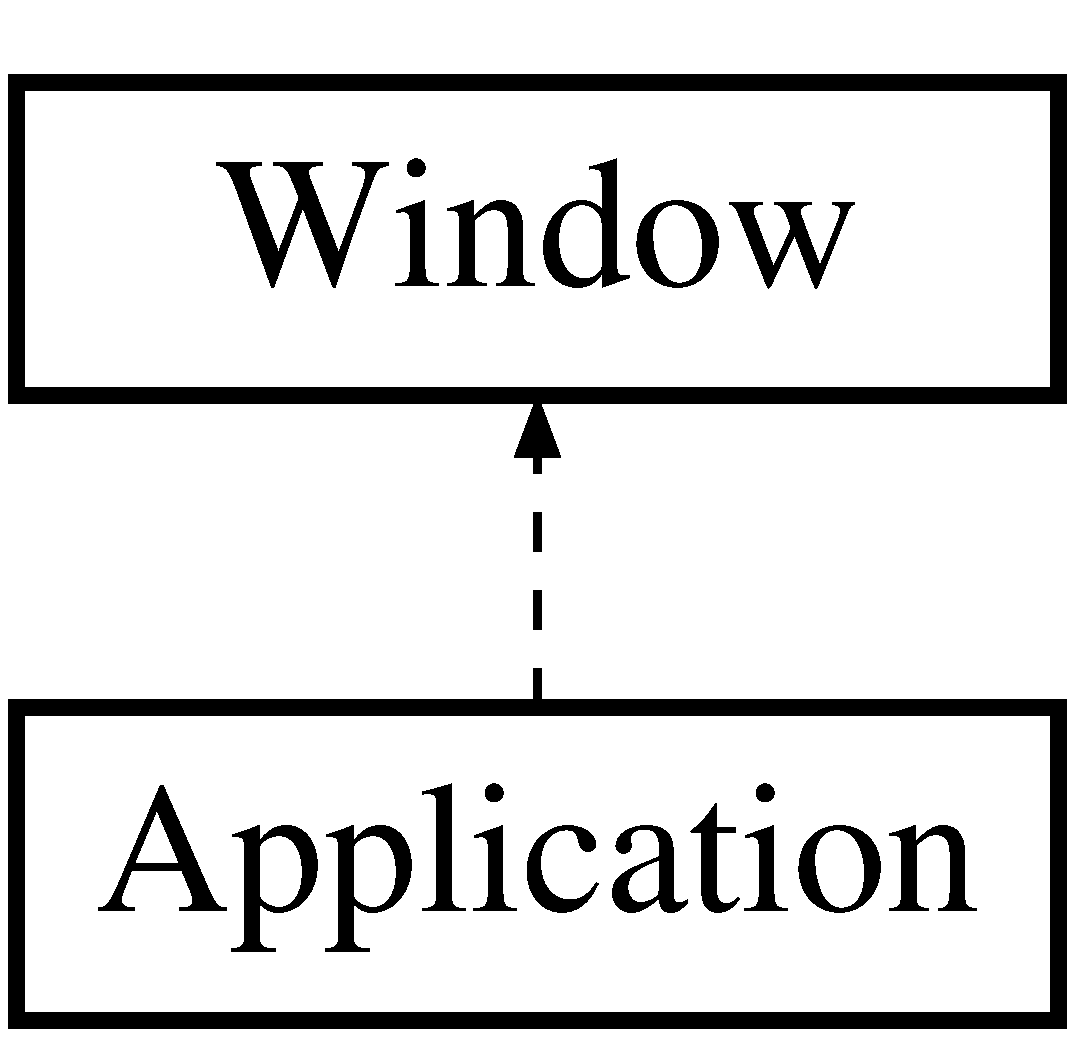
\includegraphics[height=2.000000cm]{classApplication}
\end{center}
\end{figure}
\subsection*{Public Member Functions}
\begin{DoxyCompactItemize}
\item 
\hyperlink{classApplication_a00f1777a96159f25075927bbe9076696}{Application} (int32\+\_\+t width, int32\+\_\+t height)
\begin{DoxyCompactList}\small\item\em Constructor. \end{DoxyCompactList}\item 
\mbox{\Hypertarget{classApplication_a748bca84fefb9c12661cfaa2f623748d}\label{classApplication_a748bca84fefb9c12661cfaa2f623748d}} 
\hyperlink{classApplication_a748bca84fefb9c12661cfaa2f623748d}{$\sim$\+Application} ()
\begin{DoxyCompactList}\small\item\em Destructor. \end{DoxyCompactList}\item 
{\footnotesize template$<$typename C\+L\+A\+SS $>$ }\\void \hyperlink{classApplication_a1ad1383c43c8d658761249d5a06e3a88}{register\+Method} (std\+::string const \&name)
\begin{DoxyCompactList}\small\item\em This method registers new rendering method into applicaion. \end{DoxyCompactList}\item 
\mbox{\Hypertarget{classApplication_aa38ca47b50935092078cef4281ab66bc}\label{classApplication_aa38ca47b50935092078cef4281ab66bc}} 
void \hyperlink{classApplication_aa38ca47b50935092078cef4281ab66bc}{start} ()
\begin{DoxyCompactList}\small\item\em Starts the main loop. \end{DoxyCompactList}\item 
void \hyperlink{classApplication_a5c018483318ffd6b3121902980e0e122}{set\+Method} (uint32\+\_\+t m)
\begin{DoxyCompactList}\small\item\em This function selects a rendering method. \end{DoxyCompactList}\end{DoxyCompactItemize}
\subsection*{Additional Inherited Members}


\subsection{Detailed Description}
\hyperlink{classApplication}{Application} class. 

\subsection{Constructor \& Destructor Documentation}
\mbox{\Hypertarget{classApplication_a00f1777a96159f25075927bbe9076696}\label{classApplication_a00f1777a96159f25075927bbe9076696}} 
\index{Application@{Application}!Application@{Application}}
\index{Application@{Application}!Application@{Application}}
\subsubsection{\texorpdfstring{Application()}{Application()}}
{\footnotesize\ttfamily Application\+::\+Application (\begin{DoxyParamCaption}\item[{int32\+\_\+t}]{width,  }\item[{int32\+\_\+t}]{height }\end{DoxyParamCaption})}



Constructor. 


\begin{DoxyParams}{Parameters}
{\em width} & width of the window \\
\hline
{\em height} & height of the window \\
\hline
\end{DoxyParams}


\subsection{Member Function Documentation}
\mbox{\Hypertarget{classApplication_a1ad1383c43c8d658761249d5a06e3a88}\label{classApplication_a1ad1383c43c8d658761249d5a06e3a88}} 
\index{Application@{Application}!register\+Method@{register\+Method}}
\index{register\+Method@{register\+Method}!Application@{Application}}
\subsubsection{\texorpdfstring{register\+Method()}{registerMethod()}}
{\footnotesize\ttfamily template$<$typename C\+L\+A\+SS $>$ \\
void Application\+::register\+Method (\begin{DoxyParamCaption}\item[{std\+::string const \&}]{name }\end{DoxyParamCaption})}



This method registers new rendering method into applicaion. 


\begin{DoxyTemplParams}{Template Parameters}
{\em C\+L\+A\+SS} & method class \\
\hline
\end{DoxyTemplParams}

\begin{DoxyParams}{Parameters}
{\em name} & name of the method \\
\hline
\end{DoxyParams}
\mbox{\Hypertarget{classApplication_a5c018483318ffd6b3121902980e0e122}\label{classApplication_a5c018483318ffd6b3121902980e0e122}} 
\index{Application@{Application}!set\+Method@{set\+Method}}
\index{set\+Method@{set\+Method}!Application@{Application}}
\subsubsection{\texorpdfstring{set\+Method()}{setMethod()}}
{\footnotesize\ttfamily void Application\+::set\+Method (\begin{DoxyParamCaption}\item[{uint32\+\_\+t}]{m }\end{DoxyParamCaption})}



This function selects a rendering method. 


\begin{DoxyParams}{Parameters}
{\em m} & method id \\
\hline
\end{DoxyParams}


The documentation for this class was generated from the following files\+:\begin{DoxyCompactItemize}
\item 
student/\hyperlink{application_8hpp}{application.\+hpp}\item 
student/\hyperlink{application_8cpp}{application.\+cpp}\end{DoxyCompactItemize}

\hypertarget{classArguments}{}\section{Arguments Class Reference}
\label{classArguments}\index{Arguments@{Arguments}}


This class parses command line arguments.  




{\ttfamily \#include $<$arguments.\+hpp$>$}

\subsection*{Public Member Functions}
\begin{DoxyCompactItemize}
\item 
\hyperlink{classArguments_a3d9dd7b675eac3c375c6b2e9bb13e896}{Arguments} (int argc, char $\ast$argv\mbox{[}$\,$\mbox{]})
\begin{DoxyCompactList}\small\item\em Constructor. \end{DoxyCompactList}\end{DoxyCompactItemize}
\subsection*{Data Fields}
\begin{DoxyCompactItemize}
\item 
\mbox{\Hypertarget{classArguments_a3ab231d51bfd73e74e92c7cc51e76410}\label{classArguments_a3ab231d51bfd73e74e92c7cc51e76410}} 
std\+::shared\+\_\+ptr$<$ argument\+Viewer\+::\+Argument\+Viewer $>$ \hyperlink{classArguments_a3ab231d51bfd73e74e92c7cc51e76410}{args}
\begin{DoxyCompactList}\small\item\em argument viewer \end{DoxyCompactList}\item 
\mbox{\Hypertarget{classArguments_af7c3d8d81ed86f17cf968e34c4ebaac3}\label{classArguments_af7c3d8d81ed86f17cf968e34c4ebaac3}} 
std\+::vector$<$ int32\+\_\+t $>$ \hyperlink{classArguments_af7c3d8d81ed86f17cf968e34c4ebaac3}{window\+Size}
\begin{DoxyCompactList}\small\item\em window size \end{DoxyCompactList}\item 
\mbox{\Hypertarget{classArguments_a9678e9bc1607e27fadce50ab428d9205}\label{classArguments_a9678e9bc1607e27fadce50ab428d9205}} 
std\+::string \hyperlink{classArguments_a9678e9bc1607e27fadce50ab428d9205}{ground\+Truth\+File} = \char`\"{}../tests/output.\+bmp\char`\"{}
\begin{DoxyCompactList}\small\item\em ground truth file \end{DoxyCompactList}\item 
\mbox{\Hypertarget{classArguments_a042cf06e99bcb9637e150b5bb281f192}\label{classArguments_a042cf06e99bcb9637e150b5bb281f192}} 
uint32\+\_\+t \hyperlink{classArguments_a042cf06e99bcb9637e150b5bb281f192}{method} = 0
\begin{DoxyCompactList}\small\item\em start with this method \end{DoxyCompactList}\item 
\mbox{\Hypertarget{classArguments_ac842663748666971780129ff56fd020f}\label{classArguments_ac842663748666971780129ff56fd020f}} 
bool \hyperlink{classArguments_ac842663748666971780129ff56fd020f}{run\+Performance\+Tests}
\begin{DoxyCompactList}\small\item\em should we run performance tests \end{DoxyCompactList}\item 
\mbox{\Hypertarget{classArguments_a6a3119fc79128d21da149e1d46884412}\label{classArguments_a6a3119fc79128d21da149e1d46884412}} 
bool \hyperlink{classArguments_a6a3119fc79128d21da149e1d46884412}{run\+Conformance\+Tests}
\begin{DoxyCompactList}\small\item\em sould we run conformance tests \end{DoxyCompactList}\item 
\mbox{\Hypertarget{classArguments_a830a8ebb96c1a04c951b6c35f014cc8d}\label{classArguments_a830a8ebb96c1a04c951b6c35f014cc8d}} 
bool \hyperlink{classArguments_a830a8ebb96c1a04c951b6c35f014cc8d}{take\+Screen\+Shot}
\begin{DoxyCompactList}\small\item\em should we take a screnshot \end{DoxyCompactList}\item 
\mbox{\Hypertarget{classArguments_a2dd49c62c3372545d834d26ae3b66a2f}\label{classArguments_a2dd49c62c3372545d834d26ae3b66a2f}} 
bool \hyperlink{classArguments_a2dd49c62c3372545d834d26ae3b66a2f}{stop} = false
\begin{DoxyCompactList}\small\item\em should we immediately stop \end{DoxyCompactList}\item 
\mbox{\Hypertarget{classArguments_a8c2fdc6e0dfb18c58314d7a736e5ca94}\label{classArguments_a8c2fdc6e0dfb18c58314d7a736e5ca94}} 
uint32\+\_\+t \hyperlink{classArguments_a8c2fdc6e0dfb18c58314d7a736e5ca94}{perf\+Tests}
\begin{DoxyCompactList}\small\item\em number of frames in performance tests \end{DoxyCompactList}\end{DoxyCompactItemize}


\subsection{Detailed Description}
This class parses command line arguments. 

\subsection{Constructor \& Destructor Documentation}
\mbox{\Hypertarget{classArguments_a3d9dd7b675eac3c375c6b2e9bb13e896}\label{classArguments_a3d9dd7b675eac3c375c6b2e9bb13e896}} 
\index{Arguments@{Arguments}!Arguments@{Arguments}}
\index{Arguments@{Arguments}!Arguments@{Arguments}}
\subsubsection{\texorpdfstring{Arguments()}{Arguments()}}
{\footnotesize\ttfamily Arguments\+::\+Arguments (\begin{DoxyParamCaption}\item[{int}]{argc,  }\item[{char $\ast$}]{argv\mbox{[}$\,$\mbox{]} }\end{DoxyParamCaption})\hspace{0.3cm}{\ttfamily [inline]}}



Constructor. 


\begin{DoxyParams}{Parameters}
{\em argc} & number of arguments \\
\hline
{\em argv\mbox{[}$\,$\mbox{]}} & arguments \\
\hline
\end{DoxyParams}


The documentation for this class was generated from the following file\+:\begin{DoxyCompactItemize}
\item 
student/\hyperlink{arguments_8hpp}{arguments.\+hpp}\end{DoxyCompactItemize}

\hypertarget{unionAttribute}{}\section{Attribute Union Reference}
\label{unionAttribute}\index{Attribute@{Attribute}}


This union represents one vertex/fragment attribute.  




{\ttfamily \#include $<$fwd.\+hpp$>$}

\subsection*{Data Fields}
\begin{DoxyCompactItemize}
\item 
\mbox{\Hypertarget{unionAttribute_a2a9e03282539207b21a9b61596e6b72c}\label{unionAttribute_a2a9e03282539207b21a9b61596e6b72c}} 
float \hyperlink{unionAttribute_a2a9e03282539207b21a9b61596e6b72c}{v1}
\begin{DoxyCompactList}\small\item\em single float \end{DoxyCompactList}\item 
\mbox{\Hypertarget{unionAttribute_aa240c263ec02c39b48d662a1c598e1fc}\label{unionAttribute_aa240c263ec02c39b48d662a1c598e1fc}} 
glm\+::vec2 \hyperlink{unionAttribute_aa240c263ec02c39b48d662a1c598e1fc}{v2}
\begin{DoxyCompactList}\small\item\em vector of two floats \end{DoxyCompactList}\item 
\mbox{\Hypertarget{unionAttribute_a7e4149eff36adcf056cb7153bfbf4c8c}\label{unionAttribute_a7e4149eff36adcf056cb7153bfbf4c8c}} 
glm\+::vec3 \hyperlink{unionAttribute_a7e4149eff36adcf056cb7153bfbf4c8c}{v3}
\begin{DoxyCompactList}\small\item\em vector of three floats \end{DoxyCompactList}\item 
\mbox{\Hypertarget{unionAttribute_ac47131c7c30814e28f0c4662a4ed2737}\label{unionAttribute_ac47131c7c30814e28f0c4662a4ed2737}} 
glm\+::vec4 \hyperlink{unionAttribute_ac47131c7c30814e28f0c4662a4ed2737}{v4} = glm\+::vec4(1.f)
\begin{DoxyCompactList}\small\item\em vector of four floats \end{DoxyCompactList}\end{DoxyCompactItemize}


\subsection{Detailed Description}
This union represents one vertex/fragment attribute. 

The documentation for this union was generated from the following file\+:\begin{DoxyCompactItemize}
\item 
student/\hyperlink{fwd_8hpp}{fwd.\+hpp}\end{DoxyCompactItemize}

\hypertarget{structBunnyVertex}{}\section{Bunny\+Vertex Struct Reference}
\label{structBunnyVertex}\index{Bunny\+Vertex@{Bunny\+Vertex}}


This structure represents vertex that contains only position and normal.  




{\ttfamily \#include $<$bunny.\+hpp$>$}

\subsection*{Data Fields}
\begin{DoxyCompactItemize}
\item 
\mbox{\Hypertarget{structBunnyVertex_a2d228a475dea955ec6c696ee545ac731}\label{structBunnyVertex_a2d228a475dea955ec6c696ee545ac731}} 
float \hyperlink{structBunnyVertex_a2d228a475dea955ec6c696ee545ac731}{position} \mbox{[}3\mbox{]}
\begin{DoxyCompactList}\small\item\em position of vertex \end{DoxyCompactList}\item 
\mbox{\Hypertarget{structBunnyVertex_aa7f67904a835c896f368dd2e37cc46db}\label{structBunnyVertex_aa7f67904a835c896f368dd2e37cc46db}} 
float \hyperlink{structBunnyVertex_aa7f67904a835c896f368dd2e37cc46db}{normal} \mbox{[}3\mbox{]}
\begin{DoxyCompactList}\small\item\em normal of vertex \end{DoxyCompactList}\end{DoxyCompactItemize}


\subsection{Detailed Description}
This structure represents vertex that contains only position and normal. 

The documentation for this struct was generated from the following file\+:\begin{DoxyCompactItemize}
\item 
student/\hyperlink{bunny_8hpp}{bunny.\+hpp}\end{DoxyCompactItemize}

\hypertarget{classCZFlagMethod}{}\section{C\+Z\+Flag\+Method Class Reference}
\label{classCZFlagMethod}\index{C\+Z\+Flag\+Method@{C\+Z\+Flag\+Method}}


Czech flag rendering method.  




{\ttfamily \#include $<$cz\+Flag\+Method.\+hpp$>$}

Inheritance diagram for C\+Z\+Flag\+Method\+:\begin{figure}[H]
\begin{center}
\leavevmode
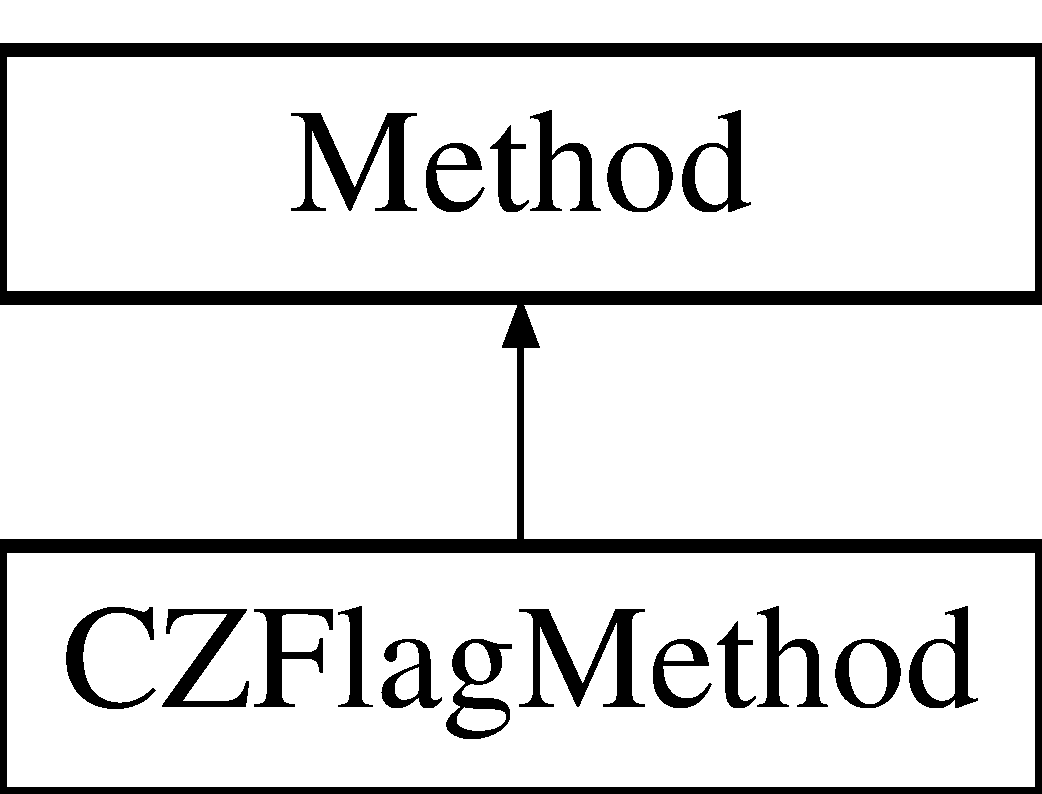
\includegraphics[height=2.000000cm]{classCZFlagMethod}
\end{center}
\end{figure}
\subsection*{Public Member Functions}
\begin{DoxyCompactItemize}
\item 
virtual void \hyperlink{classCZFlagMethod_a72425a172b48b3f730b9b8c7745cc70a}{on\+Draw} (glm\+::mat4 const \&proj, glm\+::mat4 const \&view, glm\+::vec3 const \&light, glm\+::vec3 const \&camera) override
\begin{DoxyCompactList}\small\item\em This functino is called every frame. \end{DoxyCompactList}\item 
virtual void \hyperlink{classCZFlagMethod_a337cf1158aca2ecf975fee2631071411}{on\+Update} (float dt) override
\begin{DoxyCompactList}\small\item\em This function is called on update. \end{DoxyCompactList}\end{DoxyCompactItemize}
\subsection*{Data Fields}
\begin{DoxyCompactItemize}
\item 
\mbox{\Hypertarget{classCZFlagMethod_a12d43d5482de95694d146b9a2df98fdf}\label{classCZFlagMethod_a12d43d5482de95694d146b9a2df98fdf}} 
\hyperlink{fwd_8hpp_a46ffd067c21ab50f5f1fcfed5d8bfc15}{Program\+ID} \hyperlink{classCZFlagMethod_a12d43d5482de95694d146b9a2df98fdf}{prg}
\begin{DoxyCompactList}\small\item\em id of program \end{DoxyCompactList}\item 
\mbox{\Hypertarget{classCZFlagMethod_ae12697c090cc02a88e6889294f584f6c}\label{classCZFlagMethod_ae12697c090cc02a88e6889294f584f6c}} 
\hyperlink{fwd_8hpp_af6f78f73099477c9ce5537d657597486}{Vertex\+Puller\+ID} \hyperlink{classCZFlagMethod_ae12697c090cc02a88e6889294f584f6c}{vao}
\begin{DoxyCompactList}\small\item\em id of vertex puller \end{DoxyCompactList}\item 
\mbox{\Hypertarget{classCZFlagMethod_afb718b24827f950ea22155f6e0494f8d}\label{classCZFlagMethod_afb718b24827f950ea22155f6e0494f8d}} 
\hyperlink{fwd_8hpp_a5114031b77b80ad895eff688720b7f93}{Buffer\+ID} \hyperlink{classCZFlagMethod_afb718b24827f950ea22155f6e0494f8d}{vbo}
\begin{DoxyCompactList}\small\item\em vertex buffer \end{DoxyCompactList}\item 
\mbox{\Hypertarget{classCZFlagMethod_a440e125079baaa5643564c4e0b0d335e}\label{classCZFlagMethod_a440e125079baaa5643564c4e0b0d335e}} 
\hyperlink{fwd_8hpp_a5114031b77b80ad895eff688720b7f93}{Buffer\+ID} \hyperlink{classCZFlagMethod_a440e125079baaa5643564c4e0b0d335e}{ebo}
\begin{DoxyCompactList}\small\item\em index buffer \end{DoxyCompactList}\item 
\mbox{\Hypertarget{classCZFlagMethod_a7cd60dc6b4da7b084ad7385476c6334b}\label{classCZFlagMethod_a7cd60dc6b4da7b084ad7385476c6334b}} 
float \hyperlink{classCZFlagMethod_a7cd60dc6b4da7b084ad7385476c6334b}{time} = 0.f
\begin{DoxyCompactList}\small\item\em elapsed time \end{DoxyCompactList}\item 
\mbox{\Hypertarget{classCZFlagMethod_ad9bf715285c16dac0f9c6018431abf61}\label{classCZFlagMethod_ad9bf715285c16dac0f9c6018431abf61}} 
uint32\+\_\+t const \hyperlink{classCZFlagMethod_ad9bf715285c16dac0f9c6018431abf61}{NX} = 100
\begin{DoxyCompactList}\small\item\em nof vertices in x direction \end{DoxyCompactList}\item 
\mbox{\Hypertarget{classCZFlagMethod_aa0e93166f0ed7d7ecc6e22f105a43020}\label{classCZFlagMethod_aa0e93166f0ed7d7ecc6e22f105a43020}} 
uint32\+\_\+t const \hyperlink{classCZFlagMethod_aa0e93166f0ed7d7ecc6e22f105a43020}{NY} = 10
\begin{DoxyCompactList}\small\item\em nof vertices in y direction \end{DoxyCompactList}\end{DoxyCompactItemize}


\subsection{Detailed Description}
Czech flag rendering method. 

\subsection{Member Function Documentation}
\mbox{\Hypertarget{classCZFlagMethod_a72425a172b48b3f730b9b8c7745cc70a}\label{classCZFlagMethod_a72425a172b48b3f730b9b8c7745cc70a}} 
\index{C\+Z\+Flag\+Method@{C\+Z\+Flag\+Method}!on\+Draw@{on\+Draw}}
\index{on\+Draw@{on\+Draw}!C\+Z\+Flag\+Method@{C\+Z\+Flag\+Method}}
\subsubsection{\texorpdfstring{on\+Draw()}{onDraw()}}
{\footnotesize\ttfamily void C\+Z\+Flag\+Method\+::on\+Draw (\begin{DoxyParamCaption}\item[{glm\+::mat4 const \&}]{proj,  }\item[{glm\+::mat4 const \&}]{view,  }\item[{glm\+::vec3 const \&}]{light,  }\item[{glm\+::vec3 const \&}]{camera }\end{DoxyParamCaption})\hspace{0.3cm}{\ttfamily [override]}, {\ttfamily [virtual]}}



This functino is called every frame. 


\begin{DoxyParams}{Parameters}
{\em proj} & projection matrix \\
\hline
{\em view} & view matrix \\
\hline
{\em light} & light position \\
\hline
{\em camera} & camera position \\
\hline
\end{DoxyParams}


Implements \hyperlink{classMethod_ab07a971e2a1b04a658467c643423c347}{Method}.

\mbox{\Hypertarget{classCZFlagMethod_a337cf1158aca2ecf975fee2631071411}\label{classCZFlagMethod_a337cf1158aca2ecf975fee2631071411}} 
\index{C\+Z\+Flag\+Method@{C\+Z\+Flag\+Method}!on\+Update@{on\+Update}}
\index{on\+Update@{on\+Update}!C\+Z\+Flag\+Method@{C\+Z\+Flag\+Method}}
\subsubsection{\texorpdfstring{on\+Update()}{onUpdate()}}
{\footnotesize\ttfamily void C\+Z\+Flag\+Method\+::on\+Update (\begin{DoxyParamCaption}\item[{float}]{dt }\end{DoxyParamCaption})\hspace{0.3cm}{\ttfamily [override]}, {\ttfamily [virtual]}}



This function is called on update. 


\begin{DoxyParams}{Parameters}
{\em dt} & delta time -\/ time between frames \\
\hline
\end{DoxyParams}


Reimplemented from \hyperlink{classMethod_a42dbfcfce68e920f7e957f737e93e698}{Method}.



The documentation for this class was generated from the following files\+:\begin{DoxyCompactItemize}
\item 
student/\hyperlink{czFlagMethod_8hpp}{cz\+Flag\+Method.\+hpp}\item 
student/\hyperlink{czFlagMethod_8cpp}{cz\+Flag\+Method.\+cpp}\end{DoxyCompactItemize}

\hypertarget{classEmptyMethod}{}\section{Empty\+Method Class Reference}
\label{classEmptyMethod}\index{Empty\+Method@{Empty\+Method}}


Empty rendering method.  




{\ttfamily \#include $<$empty\+Method.\+hpp$>$}

Inheritance diagram for Empty\+Method\+:\begin{figure}[H]
\begin{center}
\leavevmode
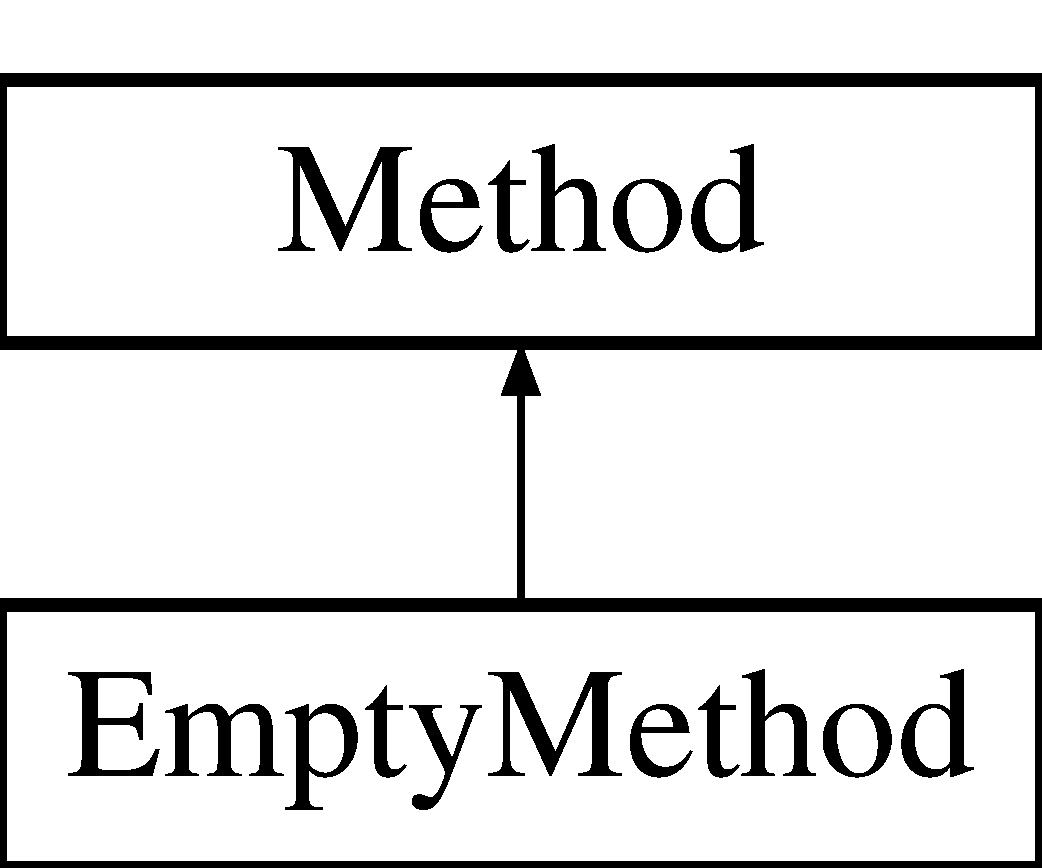
\includegraphics[height=2.000000cm]{classEmptyMethod}
\end{center}
\end{figure}
\subsection*{Public Member Functions}
\begin{DoxyCompactItemize}
\item 
virtual void \hyperlink{classEmptyMethod_a2f0962a5a3c39614b1112c137b0efd62}{on\+Draw} (glm\+::mat4 const \&proj, glm\+::mat4 const \&view, glm\+::vec3 const \&light, glm\+::vec3 const \&camera) override
\begin{DoxyCompactList}\small\item\em This functino is called every frame. \end{DoxyCompactList}\end{DoxyCompactItemize}
\subsection*{Additional Inherited Members}


\subsection{Detailed Description}
Empty rendering method. 

\subsection{Member Function Documentation}
\mbox{\Hypertarget{classEmptyMethod_a2f0962a5a3c39614b1112c137b0efd62}\label{classEmptyMethod_a2f0962a5a3c39614b1112c137b0efd62}} 
\index{Empty\+Method@{Empty\+Method}!on\+Draw@{on\+Draw}}
\index{on\+Draw@{on\+Draw}!Empty\+Method@{Empty\+Method}}
\subsubsection{\texorpdfstring{on\+Draw()}{onDraw()}}
{\footnotesize\ttfamily void Empty\+Method\+::on\+Draw (\begin{DoxyParamCaption}\item[{glm\+::mat4 const \&}]{proj,  }\item[{glm\+::mat4 const \&}]{view,  }\item[{glm\+::vec3 const \&}]{light,  }\item[{glm\+::vec3 const \&}]{camera }\end{DoxyParamCaption})\hspace{0.3cm}{\ttfamily [override]}, {\ttfamily [virtual]}}



This functino is called every frame. 


\begin{DoxyParams}{Parameters}
{\em proj} & projection matrix \\
\hline
{\em view} & view matrix \\
\hline
{\em light} & light position \\
\hline
{\em camera} & camera position \\
\hline
\end{DoxyParams}


Implements \hyperlink{classMethod_ab07a971e2a1b04a658467c643423c347}{Method}.



The documentation for this class was generated from the following file\+:\begin{DoxyCompactItemize}
\item 
student/\hyperlink{emptyMethod_8hpp}{empty\+Method.\+hpp}\end{DoxyCompactItemize}

\hypertarget{classGPU}{}\section{G\+PU Class Reference}
\label{classGPU}\index{G\+PU@{G\+PU}}


This class represent software \hyperlink{classGPU}{G\+PU}.  




{\ttfamily \#include $<$gpu.\+hpp$>$}

\subsection*{Public Member Functions}
\begin{DoxyCompactItemize}
\item 
\hyperlink{group__gpu__init_ga2ca7973e32f63ba3472166a007419a75}{G\+PU} ()
\begin{DoxyCompactList}\small\item\em Constructor of \hyperlink{classGPU}{G\+PU}. \end{DoxyCompactList}\item 
virtual \hyperlink{group__gpu__init_gac4d153a08d3b9f40e5a8f1634f4a9e78}{$\sim$\+G\+PU} ()
\begin{DoxyCompactList}\small\item\em Destructor of \hyperlink{classGPU}{G\+PU}. \end{DoxyCompactList}\item 
\hyperlink{fwd_8hpp_a5114031b77b80ad895eff688720b7f93}{Buffer\+ID} \hyperlink{group__buffer__tasks_ga309724692e0d90a686642379f12d8d44}{create\+Buffer} (uint64\+\_\+t size)
\begin{DoxyCompactList}\small\item\em This function allocates buffer on \hyperlink{classGPU}{G\+PU}. \end{DoxyCompactList}\item 
void \hyperlink{group__buffer__tasks_ga05fb19b7c8b51a92162517aa7f25a166}{delete\+Buffer} (\hyperlink{fwd_8hpp_a5114031b77b80ad895eff688720b7f93}{Buffer\+ID} buffer)
\begin{DoxyCompactList}\small\item\em This function frees allocated buffer on \hyperlink{classGPU}{G\+PU}. \end{DoxyCompactList}\item 
void \hyperlink{group__buffer__tasks_ga97e1e76065fd913d6624b4c03164dcec}{set\+Buffer\+Data} (\hyperlink{fwd_8hpp_a5114031b77b80ad895eff688720b7f93}{Buffer\+ID} buffer, uint64\+\_\+t offset, uint64\+\_\+t size, void const $\ast$data)
\begin{DoxyCompactList}\small\item\em This function uploads data to selected buffer on the \hyperlink{classGPU}{G\+PU}. \end{DoxyCompactList}\item 
void \hyperlink{group__buffer__tasks_ga7b89dbe4afbfec3725c64000b37445af}{get\+Buffer\+Data} (\hyperlink{fwd_8hpp_a5114031b77b80ad895eff688720b7f93}{Buffer\+ID} buffer, uint64\+\_\+t offset, uint64\+\_\+t size, void $\ast$data)
\begin{DoxyCompactList}\small\item\em This function downloads data from \hyperlink{classGPU}{G\+PU}. \end{DoxyCompactList}\item 
bool \hyperlink{group__buffer__tasks_gae725a1955d617a7e655ab751c6e05e97}{is\+Buffer} (\hyperlink{fwd_8hpp_a5114031b77b80ad895eff688720b7f93}{Buffer\+ID} buffer)
\begin{DoxyCompactList}\small\item\em This function tests if buffer exists. \end{DoxyCompactList}\item 
\hyperlink{fwd_8hpp_af56aa505d50bcd62e9e9c5a72564af4d}{Object\+ID} \hyperlink{group__vertexpuller__tasks_gaabe965c10fea7cd8f8af3aa528915c92}{create\+Vertex\+Puller} ()
\begin{DoxyCompactList}\small\item\em This function creates new vertex puller settings on the \hyperlink{classGPU}{G\+PU},. \end{DoxyCompactList}\item 
void \hyperlink{group__vertexpuller__tasks_gadf91a9fec77d8d23f093458b36a733fc}{delete\+Vertex\+Puller} (\hyperlink{fwd_8hpp_af6f78f73099477c9ce5537d657597486}{Vertex\+Puller\+ID} vao)
\begin{DoxyCompactList}\small\item\em This function deletes vertex puller settings. \end{DoxyCompactList}\item 
void \hyperlink{group__vertexpuller__tasks_gae9ffbcfa3b43ac9b3ea53e5bc44f83cc}{set\+Vertex\+Puller\+Head} (\hyperlink{fwd_8hpp_af6f78f73099477c9ce5537d657597486}{Vertex\+Puller\+ID} vao, uint32\+\_\+t head, \hyperlink{fwd_8hpp_a349a9cde14be8097df865ba0469c0ab2}{Attribute\+Type} type, uint64\+\_\+t stride, uint64\+\_\+t offset, \hyperlink{fwd_8hpp_a5114031b77b80ad895eff688720b7f93}{Buffer\+ID} buffer)
\begin{DoxyCompactList}\small\item\em This function sets one vertex puller reading head. \end{DoxyCompactList}\item 
void \hyperlink{group__vertexpuller__tasks_gae5238dbc60eb2ece94df110945a4f46b}{set\+Vertex\+Puller\+Indexing} (\hyperlink{fwd_8hpp_af6f78f73099477c9ce5537d657597486}{Vertex\+Puller\+ID} vao, \hyperlink{fwd_8hpp_a2bfb0a0ff1c379a8b4e8f9d24fdd4839}{Index\+Type} type, \hyperlink{fwd_8hpp_a5114031b77b80ad895eff688720b7f93}{Buffer\+ID} buffer)
\begin{DoxyCompactList}\small\item\em This function sets vertex puller indexing. \end{DoxyCompactList}\item 
void \hyperlink{group__vertexpuller__tasks_ga61384d99754bda4d91790c49b1639b30}{enable\+Vertex\+Puller\+Head} (\hyperlink{fwd_8hpp_af6f78f73099477c9ce5537d657597486}{Vertex\+Puller\+ID} vao, uint32\+\_\+t head)
\begin{DoxyCompactList}\small\item\em This function enables vertex puller\textquotesingle{}s head. \end{DoxyCompactList}\item 
void \hyperlink{group__vertexpuller__tasks_gae95cab56d80cb888e71b25965dc868c5}{disable\+Vertex\+Puller\+Head} (\hyperlink{fwd_8hpp_af6f78f73099477c9ce5537d657597486}{Vertex\+Puller\+ID} vao, uint32\+\_\+t head)
\begin{DoxyCompactList}\small\item\em This function disables vertex puller\textquotesingle{}s head. \end{DoxyCompactList}\item 
void \hyperlink{group__vertexpuller__tasks_gac7f9799e1a6a3b1cafb5f4c4c5e9555d}{bind\+Vertex\+Puller} (\hyperlink{fwd_8hpp_af6f78f73099477c9ce5537d657597486}{Vertex\+Puller\+ID} vao)
\begin{DoxyCompactList}\small\item\em This function selects active vertex puller. \end{DoxyCompactList}\item 
void \hyperlink{group__vertexpuller__tasks_gafdfb7e3cd24d595af6650b68ba9f6f24}{unbind\+Vertex\+Puller} ()
\begin{DoxyCompactList}\small\item\em This function deactivates vertex puller. \end{DoxyCompactList}\item 
bool \hyperlink{group__vertexpuller__tasks_ga09408b5ca4250292217f3330ae674319}{is\+Vertex\+Puller} (\hyperlink{fwd_8hpp_af6f78f73099477c9ce5537d657597486}{Vertex\+Puller\+ID} vao)
\begin{DoxyCompactList}\small\item\em This function tests if vertex puller exists. \end{DoxyCompactList}\item 
\hyperlink{fwd_8hpp_a46ffd067c21ab50f5f1fcfed5d8bfc15}{Program\+ID} \hyperlink{group__program__tasks_gae1368a616ba5be607b9cf4dd1e60dfe0}{create\+Program} ()
\begin{DoxyCompactList}\small\item\em This function creates new shader program. \end{DoxyCompactList}\item 
void \hyperlink{group__program__tasks_ga3f8363f9c27c3f900f258e6acee52683}{delete\+Program} (\hyperlink{fwd_8hpp_a46ffd067c21ab50f5f1fcfed5d8bfc15}{Program\+ID} prg)
\begin{DoxyCompactList}\small\item\em This function deletes shader program. \end{DoxyCompactList}\item 
void \hyperlink{group__program__tasks_gafe72b55028369d1e9e9f8d087c76af09}{attach\+Shaders} (\hyperlink{fwd_8hpp_a46ffd067c21ab50f5f1fcfed5d8bfc15}{Program\+ID} prg, \hyperlink{fwd_8hpp_af647cdb302d7e978c6a0da41a0a92725}{Vertex\+Shader} vs, \hyperlink{fwd_8hpp_a52f1704ae0b129e49fe1902e05319ad6}{Fragment\+Shader} fs)
\begin{DoxyCompactList}\small\item\em This function attaches vertex and frament shader to shader program. \end{DoxyCompactList}\item 
void \hyperlink{group__program__tasks_gaff499d4f692ea0dd7125bfd324957619}{set\+V\+S2\+F\+S\+Type} (\hyperlink{fwd_8hpp_a46ffd067c21ab50f5f1fcfed5d8bfc15}{Program\+ID} prg, uint32\+\_\+t attrib, \hyperlink{fwd_8hpp_a349a9cde14be8097df865ba0469c0ab2}{Attribute\+Type} type)
\begin{DoxyCompactList}\small\item\em This function selects which vertex attributes should be interpolated during rasterization into fragment attributes. \end{DoxyCompactList}\item 
void \hyperlink{group__program__tasks_ga4f2bd468b0ef5fed61ffa34314319a20}{use\+Program} (\hyperlink{fwd_8hpp_a46ffd067c21ab50f5f1fcfed5d8bfc15}{Program\+ID} prg)
\begin{DoxyCompactList}\small\item\em This function actives selected shader program. \end{DoxyCompactList}\item 
bool \hyperlink{group__program__tasks_ga481c0eb5be3150af401a58fa167506e0}{is\+Program} (\hyperlink{fwd_8hpp_a46ffd067c21ab50f5f1fcfed5d8bfc15}{Program\+ID} prg)
\begin{DoxyCompactList}\small\item\em This function tests if selected shader program exists. \end{DoxyCompactList}\item 
void \hyperlink{group__program__tasks_gaa9e9717db5520e6c34a1b380d6321758}{program\+Uniform1f} (\hyperlink{fwd_8hpp_a46ffd067c21ab50f5f1fcfed5d8bfc15}{Program\+ID} prg, uint32\+\_\+t uniform\+Id, float const \&d)
\begin{DoxyCompactList}\small\item\em This function sets uniform value (1 float). \end{DoxyCompactList}\item 
void \hyperlink{group__program__tasks_gac34e13783980686c497adda156923b1d}{program\+Uniform2f} (\hyperlink{fwd_8hpp_a46ffd067c21ab50f5f1fcfed5d8bfc15}{Program\+ID} prg, uint32\+\_\+t uniform\+Id, glm\+::vec2 const \&d)
\begin{DoxyCompactList}\small\item\em This function sets uniform value (2 float). \end{DoxyCompactList}\item 
void \hyperlink{group__program__tasks_ga06b1aca1375a9cfff13d3b66defe485f}{program\+Uniform3f} (\hyperlink{fwd_8hpp_a46ffd067c21ab50f5f1fcfed5d8bfc15}{Program\+ID} prg, uint32\+\_\+t uniform\+Id, glm\+::vec3 const \&d)
\begin{DoxyCompactList}\small\item\em This function sets uniform value (3 float). \end{DoxyCompactList}\item 
void \hyperlink{group__program__tasks_gad703e87e1652a78261739c6b5108c852}{program\+Uniform4f} (\hyperlink{fwd_8hpp_a46ffd067c21ab50f5f1fcfed5d8bfc15}{Program\+ID} prg, uint32\+\_\+t uniform\+Id, glm\+::vec4 const \&d)
\begin{DoxyCompactList}\small\item\em This function sets uniform value (4 float). \end{DoxyCompactList}\item 
void \hyperlink{group__program__tasks_gac3b490a674226c0510ac3c0b784010fa}{program\+Uniform\+Matrix4f} (\hyperlink{fwd_8hpp_a46ffd067c21ab50f5f1fcfed5d8bfc15}{Program\+ID} prg, uint32\+\_\+t uniform\+Id, glm\+::mat4 const \&d)
\begin{DoxyCompactList}\small\item\em This function sets uniform value (4 float). \end{DoxyCompactList}\item 
void \hyperlink{group__framebuffer__tasks_gab041c171fc07011d13ec608fc94a1d1c}{create\+Framebuffer} (uint32\+\_\+t width, uint32\+\_\+t height)
\begin{DoxyCompactList}\small\item\em This function creates framebuffer on \hyperlink{classGPU}{G\+PU}. \end{DoxyCompactList}\item 
void \hyperlink{group__framebuffer__tasks_gaaaa9fbf5f3c28f27f092c2c6883d6e60}{delete\+Framebuffer} ()
\begin{DoxyCompactList}\small\item\em This function deletes framebuffer. \end{DoxyCompactList}\item 
void \hyperlink{group__framebuffer__tasks_ga6391eaf70194c39bf523ddc875ca176d}{resize\+Framebuffer} (uint32\+\_\+t width, uint32\+\_\+t height)
\begin{DoxyCompactList}\small\item\em This function resizes framebuffer. \end{DoxyCompactList}\item 
uint8\+\_\+t $\ast$ \hyperlink{group__framebuffer__tasks_ga67504b8136ef6283ad6efbb5323a0ef8}{get\+Framebuffer\+Color} ()
\begin{DoxyCompactList}\small\item\em This function returns pointer to color buffer. \end{DoxyCompactList}\item 
float $\ast$ \hyperlink{group__framebuffer__tasks_gab755d51ff9686df1fb9b2892b9861c1d}{get\+Framebuffer\+Depth} ()
\begin{DoxyCompactList}\small\item\em This function returns pointer to depth buffer. \end{DoxyCompactList}\item 
uint32\+\_\+t \hyperlink{group__framebuffer__tasks_ga467b565d440e5742b7ebc104a2d70ce3}{get\+Framebuffer\+Width} ()
\begin{DoxyCompactList}\small\item\em This function returns width of framebuffer. \end{DoxyCompactList}\item 
uint32\+\_\+t \hyperlink{group__framebuffer__tasks_gaa115f7153407b8020fd153b71abccf0e}{get\+Framebuffer\+Height} ()
\begin{DoxyCompactList}\small\item\em This function returns height of framebuffer. \end{DoxyCompactList}\item 
void \hyperlink{group__draw__tasks_ga012ff10197fb3e5051b854a0028db31d}{clear} (float r, float g, float b, float a)
\begin{DoxyCompactList}\small\item\em This functino clears framebuffer. \end{DoxyCompactList}\item 
void \hyperlink{group__draw__tasks_ga127436afbcbda852746dfb9dae885ecf}{draw\+Triangles} (uint32\+\_\+t nof\+Vertices)
\end{DoxyCompactItemize}


\subsection{Detailed Description}
This class represent software \hyperlink{classGPU}{G\+PU}. 

The documentation for this class was generated from the following files\+:\begin{DoxyCompactItemize}
\item 
student/\hyperlink{gpu_8hpp}{gpu.\+hpp}\item 
student/\hyperlink{gpu_8cpp}{gpu.\+cpp}\end{DoxyCompactItemize}

\hypertarget{structInFragment}{}\section{In\+Fragment Struct Reference}
\label{structInFragment}\index{In\+Fragment@{In\+Fragment}}


This struct represents input fragment.  




{\ttfamily \#include $<$fwd.\+hpp$>$}

\subsection*{Data Fields}
\begin{DoxyCompactItemize}
\item 
\mbox{\Hypertarget{structInFragment_af9cd9e9a684a1c454d52d7e191564be1}\label{structInFragment_af9cd9e9a684a1c454d52d7e191564be1}} 
\hyperlink{unionAttribute}{Attribute} \hyperlink{structInFragment_af9cd9e9a684a1c454d52d7e191564be1}{attributes} \mbox{[}\hyperlink{fwd_8hpp_a176b31bcc8f8b93ee7ef0810ea77730b}{max\+Attributes}\mbox{]}
\begin{DoxyCompactList}\small\item\em fragment attributes \end{DoxyCompactList}\item 
\mbox{\Hypertarget{structInFragment_ae72e0b96e17181ea2cb2ef256e3f0a8f}\label{structInFragment_ae72e0b96e17181ea2cb2ef256e3f0a8f}} 
glm\+::vec4 \hyperlink{structInFragment_ae72e0b96e17181ea2cb2ef256e3f0a8f}{gl\+\_\+\+Frag\+Coord}
\begin{DoxyCompactList}\small\item\em fragment coordinates \end{DoxyCompactList}\end{DoxyCompactItemize}


\subsection{Detailed Description}
This struct represents input fragment. 

The documentation for this struct was generated from the following file\+:\begin{DoxyCompactItemize}
\item 
student/\hyperlink{fwd_8hpp}{fwd.\+hpp}\end{DoxyCompactItemize}

\hypertarget{structInVertex}{}\section{In\+Vertex Struct Reference}
\label{structInVertex}\index{In\+Vertex@{In\+Vertex}}


This struct represents input vertex of vertex shader.  




{\ttfamily \#include $<$fwd.\+hpp$>$}

\subsection*{Data Fields}
\begin{DoxyCompactItemize}
\item 
\mbox{\Hypertarget{structInVertex_a4fc269d49110daa41aedf9b8f313f0ca}\label{structInVertex_a4fc269d49110daa41aedf9b8f313f0ca}} 
\hyperlink{unionAttribute}{Attribute} \hyperlink{structInVertex_a4fc269d49110daa41aedf9b8f313f0ca}{attributes} \mbox{[}\hyperlink{fwd_8hpp_a176b31bcc8f8b93ee7ef0810ea77730b}{max\+Attributes}\mbox{]}
\begin{DoxyCompactList}\small\item\em vertex attributes \end{DoxyCompactList}\item 
\mbox{\Hypertarget{structInVertex_aa4d31911053492bffe4b41dae12ee000}\label{structInVertex_aa4d31911053492bffe4b41dae12ee000}} 
uint32\+\_\+t \hyperlink{structInVertex_aa4d31911053492bffe4b41dae12ee000}{gl\+\_\+\+Vertex\+ID}
\begin{DoxyCompactList}\small\item\em vertex id \end{DoxyCompactList}\end{DoxyCompactItemize}


\subsection{Detailed Description}
This struct represents input vertex of vertex shader. 

The documentation for this struct was generated from the following file\+:\begin{DoxyCompactItemize}
\item 
student/\hyperlink{fwd_8hpp}{fwd.\+hpp}\end{DoxyCompactItemize}

\hypertarget{classMethod}{}\section{Method Class Reference}
\label{classMethod}\index{Method@{Method}}


This class represents rendering method.  




{\ttfamily \#include $<$method.\+hpp$>$}

Inheritance diagram for Method\+:\begin{figure}[H]
\begin{center}
\leavevmode
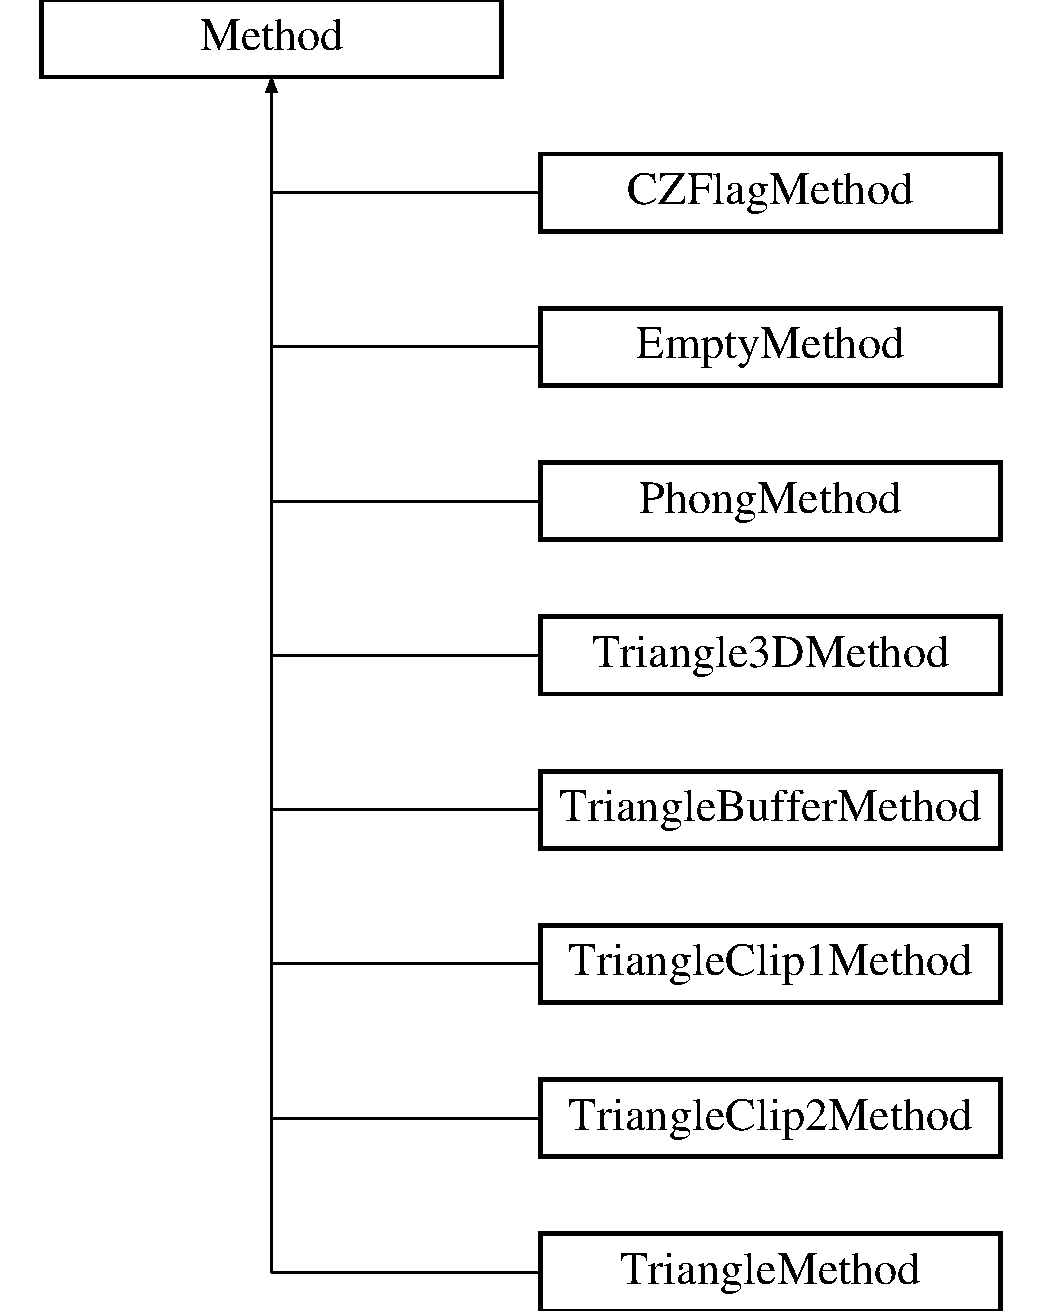
\includegraphics[height=9.000000cm]{classMethod}
\end{center}
\end{figure}
\subsection*{Public Member Functions}
\begin{DoxyCompactItemize}
\item 
\mbox{\Hypertarget{classMethod_ab48717dc68d3c057b65574a539a480f7}\label{classMethod_ab48717dc68d3c057b65574a539a480f7}} 
\hyperlink{classMethod_ab48717dc68d3c057b65574a539a480f7}{Method} ()
\begin{DoxyCompactList}\small\item\em Constructor of rendering method. \end{DoxyCompactList}\item 
\mbox{\Hypertarget{classMethod_aa4e3f9623f9a67d2e3b3017fd8aa8264}\label{classMethod_aa4e3f9623f9a67d2e3b3017fd8aa8264}} 
virtual \hyperlink{classMethod_aa4e3f9623f9a67d2e3b3017fd8aa8264}{$\sim$\+Method} ()
\begin{DoxyCompactList}\small\item\em Destructor of rendering method. \end{DoxyCompactList}\item 
virtual void \hyperlink{classMethod_ab07a971e2a1b04a658467c643423c347}{on\+Draw} (glm\+::mat4 const \&proj, glm\+::mat4 const \&view, glm\+::vec3 const \&light, glm\+::vec3 const \&camera)=0
\begin{DoxyCompactList}\small\item\em This functino is called every frame. \end{DoxyCompactList}\item 
virtual void \hyperlink{classMethod_a42dbfcfce68e920f7e957f737e93e698}{on\+Update} (float dt)
\begin{DoxyCompactList}\small\item\em This function is called on update. \end{DoxyCompactList}\end{DoxyCompactItemize}
\subsection*{Data Fields}
\begin{DoxyCompactItemize}
\item 
\mbox{\Hypertarget{classMethod_a60dbb554906836cd162036be07ab1c87}\label{classMethod_a60dbb554906836cd162036be07ab1c87}} 
\hyperlink{classGPU}{G\+PU} \hyperlink{classMethod_a60dbb554906836cd162036be07ab1c87}{gpu}
\begin{DoxyCompactList}\small\item\em graphic card \end{DoxyCompactList}\end{DoxyCompactItemize}


\subsection{Detailed Description}
This class represents rendering method. 

\subsection{Member Function Documentation}
\mbox{\Hypertarget{classMethod_ab07a971e2a1b04a658467c643423c347}\label{classMethod_ab07a971e2a1b04a658467c643423c347}} 
\index{Method@{Method}!on\+Draw@{on\+Draw}}
\index{on\+Draw@{on\+Draw}!Method@{Method}}
\subsubsection{\texorpdfstring{on\+Draw()}{onDraw()}}
{\footnotesize\ttfamily virtual void Method\+::on\+Draw (\begin{DoxyParamCaption}\item[{glm\+::mat4 const \&}]{proj,  }\item[{glm\+::mat4 const \&}]{view,  }\item[{glm\+::vec3 const \&}]{light,  }\item[{glm\+::vec3 const \&}]{camera }\end{DoxyParamCaption})\hspace{0.3cm}{\ttfamily [pure virtual]}}



This functino is called every frame. 


\begin{DoxyParams}{Parameters}
{\em proj} & projection matrix \\
\hline
{\em view} & view matrix \\
\hline
{\em light} & light position \\
\hline
{\em camera} & camera position \\
\hline
\end{DoxyParams}


Implemented in \hyperlink{group__cpu__side_ga100e32901442800e1c155b5ce089f7c5}{Phong\+Method}, \hyperlink{classCZFlagMethod_a72425a172b48b3f730b9b8c7745cc70a}{C\+Z\+Flag\+Method}, \hyperlink{classEmptyMethod_a2f0962a5a3c39614b1112c137b0efd62}{Empty\+Method}, \hyperlink{classTriangle3DMethod_a8e006abc4a38f47bfda0263acfbb7585}{Triangle3\+D\+Method}, \hyperlink{classTriangleBufferMethod_ae4339a5479f2f4fe9ca5964d5f7f1f74}{Triangle\+Buffer\+Method}, \hyperlink{classTriangleClip1Method_a5761d061239fbd8afa2e8c29cc3bef04}{Triangle\+Clip1\+Method}, \hyperlink{classTriangleClip2Method_a8433b228a45401ae637ec6d65a047ea5}{Triangle\+Clip2\+Method}, and \hyperlink{classTriangleMethod_a92fa9c2070469055edee05594a8639c9}{Triangle\+Method}.

\mbox{\Hypertarget{classMethod_a42dbfcfce68e920f7e957f737e93e698}\label{classMethod_a42dbfcfce68e920f7e957f737e93e698}} 
\index{Method@{Method}!on\+Update@{on\+Update}}
\index{on\+Update@{on\+Update}!Method@{Method}}
\subsubsection{\texorpdfstring{on\+Update()}{onUpdate()}}
{\footnotesize\ttfamily virtual void Method\+::on\+Update (\begin{DoxyParamCaption}\item[{float}]{dt }\end{DoxyParamCaption})\hspace{0.3cm}{\ttfamily [inline]}, {\ttfamily [virtual]}}



This function is called on update. 


\begin{DoxyParams}{Parameters}
{\em dt} & delta time -\/ time between frames \\
\hline
\end{DoxyParams}


Reimplemented in \hyperlink{classCZFlagMethod_a337cf1158aca2ecf975fee2631071411}{C\+Z\+Flag\+Method}.



The documentation for this class was generated from the following file\+:\begin{DoxyCompactItemize}
\item 
student/\hyperlink{method_8hpp}{method.\+hpp}\end{DoxyCompactItemize}

\hypertarget{structOutFragment}{}\section{Out\+Fragment Struct Reference}
\label{structOutFragment}\index{Out\+Fragment@{Out\+Fragment}}


This struct represents output fragment.  




{\ttfamily \#include $<$fwd.\+hpp$>$}

\subsection*{Data Fields}
\begin{DoxyCompactItemize}
\item 
\mbox{\Hypertarget{structOutFragment_a9670bf5a31a5c23fccdbeaad959cc3cf}\label{structOutFragment_a9670bf5a31a5c23fccdbeaad959cc3cf}} 
glm\+::vec4 \hyperlink{structOutFragment_a9670bf5a31a5c23fccdbeaad959cc3cf}{gl\+\_\+\+Frag\+Color}
\begin{DoxyCompactList}\small\item\em fragment color \end{DoxyCompactList}\end{DoxyCompactItemize}


\subsection{Detailed Description}
This struct represents output fragment. 

The documentation for this struct was generated from the following file\+:\begin{DoxyCompactItemize}
\item 
student/\hyperlink{fwd_8hpp}{fwd.\+hpp}\end{DoxyCompactItemize}

\hypertarget{structOutVertex}{}\section{Out\+Vertex Struct Reference}
\label{structOutVertex}\index{Out\+Vertex@{Out\+Vertex}}


This struct represents output vertex of vertex shader.  




{\ttfamily \#include $<$fwd.\+hpp$>$}

\subsection*{Data Fields}
\begin{DoxyCompactItemize}
\item 
\mbox{\Hypertarget{structOutVertex_ad1d48203a36e3ee510841f25a5bc068e}\label{structOutVertex_ad1d48203a36e3ee510841f25a5bc068e}} 
\hyperlink{unionAttribute}{Attribute} \hyperlink{structOutVertex_ad1d48203a36e3ee510841f25a5bc068e}{attributes} \mbox{[}\hyperlink{fwd_8hpp_a176b31bcc8f8b93ee7ef0810ea77730b}{max\+Attributes}\mbox{]}
\begin{DoxyCompactList}\small\item\em vertex attributes \end{DoxyCompactList}\item 
\mbox{\Hypertarget{structOutVertex_a9ca7de8eef8d688163497a7d34c76d7b}\label{structOutVertex_a9ca7de8eef8d688163497a7d34c76d7b}} 
glm\+::vec4 \hyperlink{structOutVertex_a9ca7de8eef8d688163497a7d34c76d7b}{gl\+\_\+\+Position}
\begin{DoxyCompactList}\small\item\em clip space position \end{DoxyCompactList}\end{DoxyCompactItemize}


\subsection{Detailed Description}
This struct represents output vertex of vertex shader. 

The documentation for this struct was generated from the following file\+:\begin{DoxyCompactItemize}
\item 
student/\hyperlink{fwd_8hpp}{fwd.\+hpp}\end{DoxyCompactItemize}

\hypertarget{classPhongMethod}{}\section{Phong\+Method Class Reference}
\label{classPhongMethod}\index{Phong\+Method@{Phong\+Method}}


This class holds all variables of phong method.  




{\ttfamily \#include $<$phong\+Method.\+hpp$>$}

Inheritance diagram for Phong\+Method\+:\begin{figure}[H]
\begin{center}
\leavevmode
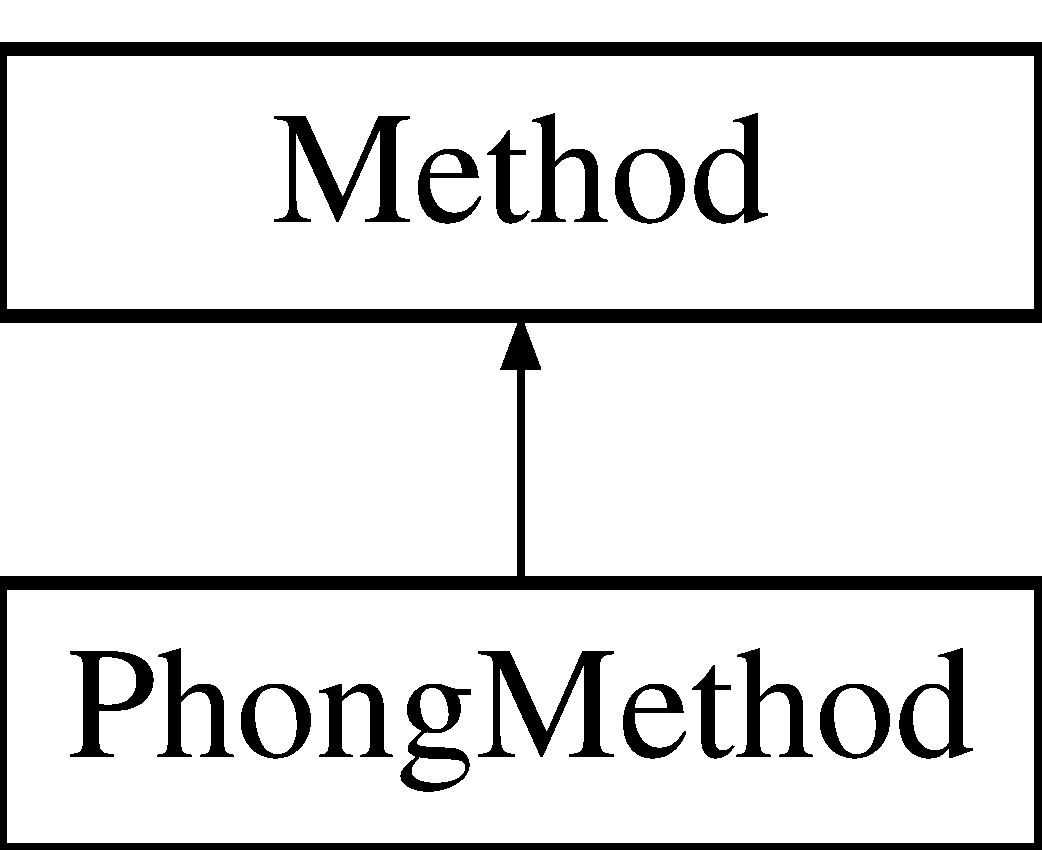
\includegraphics[height=2.000000cm]{classPhongMethod}
\end{center}
\end{figure}
\subsection*{Public Member Functions}
\begin{DoxyCompactItemize}
\item 
\hyperlink{group__cpu__side_ga609f942b12f18a74313937d4aa071c0b}{Phong\+Method} ()
\begin{DoxyCompactList}\small\item\em Constructoro f phong method. \end{DoxyCompactList}\item 
virtual \hyperlink{group__cpu__side_ga64fbf177f01aca9027d510611a2dad73}{$\sim$\+Phong\+Method} ()
\begin{DoxyCompactList}\small\item\em Destructor of phong method. \end{DoxyCompactList}\item 
virtual void \hyperlink{group__cpu__side_ga100e32901442800e1c155b5ce089f7c5}{on\+Draw} (glm\+::mat4 const \&proj, glm\+::mat4 const \&view, glm\+::vec3 const \&light, glm\+::vec3 const \&camera) override
\begin{DoxyCompactList}\small\item\em This function draws phong method. \end{DoxyCompactList}\end{DoxyCompactItemize}
\subsection*{Additional Inherited Members}


\subsection{Detailed Description}
This class holds all variables of phong method. 

The documentation for this class was generated from the following files\+:\begin{DoxyCompactItemize}
\item 
student/\hyperlink{phongMethod_8hpp}{phong\+Method.\+hpp}\item 
student/\hyperlink{phongMethod_8cpp}{phong\+Method.\+cpp}\end{DoxyCompactItemize}

\hypertarget{classTimer}{}\section{Timer$<$ T\+Y\+PE $>$ Class Template Reference}
\label{classTimer}\index{Timer$<$ T\+Y\+P\+E $>$@{Timer$<$ T\+Y\+P\+E $>$}}


This class represents a timer.  




{\ttfamily \#include $<$timer.\+hpp$>$}

\subsection*{Public Member Functions}
\begin{DoxyCompactItemize}
\item 
\mbox{\Hypertarget{classTimer_ac2eb752a6b9637733fb7eb45a57d009a}\label{classTimer_ac2eb752a6b9637733fb7eb45a57d009a}} 
\hyperlink{classTimer_ac2eb752a6b9637733fb7eb45a57d009a}{Timer} ()
\begin{DoxyCompactList}\small\item\em Construcor of timer. \end{DoxyCompactList}\item 
\mbox{\Hypertarget{classTimer_adff965ac1f6c3b04fd5e62c177662f3f}\label{classTimer_adff965ac1f6c3b04fd5e62c177662f3f}} 
void \hyperlink{classTimer_adff965ac1f6c3b04fd5e62c177662f3f}{reset} ()
\begin{DoxyCompactList}\small\item\em This function resets the timer. \end{DoxyCompactList}\item 
T\+Y\+PE \hyperlink{classTimer_ac04d0efef266558d59d647c769d2738d}{elapsed\+From\+Start} ()
\begin{DoxyCompactList}\small\item\em This function returns time elapsed from the construction of the timer. \end{DoxyCompactList}\item 
T\+Y\+PE \hyperlink{classTimer_a83d6f139a67a082e00c7ed74fcd4d83d}{elapsed\+From\+Last} ()
\begin{DoxyCompactList}\small\item\em This function returns time elapsed from the last time this function was called. \end{DoxyCompactList}\end{DoxyCompactItemize}
\subsection*{Protected Attributes}
\begin{DoxyCompactItemize}
\item 
\mbox{\Hypertarget{classTimer_a9641c1e7a368b9299dcce0ce2e790791}\label{classTimer_a9641c1e7a368b9299dcce0ce2e790791}} 
std\+::chrono\+::time\+\_\+point$<$ std\+::chrono\+::high\+\_\+resolution\+\_\+clock $>$ \hyperlink{classTimer_a9641c1e7a368b9299dcce0ce2e790791}{start}
\begin{DoxyCompactList}\small\item\em Timepoint of timer construction. \end{DoxyCompactList}\item 
\mbox{\Hypertarget{classTimer_ae0bd3fd7d2d26b40bf226e1adc3e9994}\label{classTimer_ae0bd3fd7d2d26b40bf226e1adc3e9994}} 
std\+::chrono\+::time\+\_\+point$<$ std\+::chrono\+::high\+\_\+resolution\+\_\+clock $>$ \hyperlink{classTimer_ae0bd3fd7d2d26b40bf226e1adc3e9994}{last}
\begin{DoxyCompactList}\small\item\em Timepoint of the last elapsed\+From\+Last call. \end{DoxyCompactList}\end{DoxyCompactItemize}


\subsection{Detailed Description}
\subsubsection*{template$<$typename T\+Y\+PE$>$\newline
class Timer$<$ T\+Y\+P\+E $>$}

This class represents a timer. 


\begin{DoxyTemplParams}{Template Parameters}
{\em T\+Y\+PE} & type of timer \\
\hline
\end{DoxyTemplParams}


\subsection{Member Function Documentation}
\mbox{\Hypertarget{classTimer_a83d6f139a67a082e00c7ed74fcd4d83d}\label{classTimer_a83d6f139a67a082e00c7ed74fcd4d83d}} 
\index{Timer@{Timer}!elapsed\+From\+Last@{elapsed\+From\+Last}}
\index{elapsed\+From\+Last@{elapsed\+From\+Last}!Timer@{Timer}}
\subsubsection{\texorpdfstring{elapsed\+From\+Last()}{elapsedFromLast()}}
{\footnotesize\ttfamily template$<$typename T\+Y\+PE$>$ \\
T\+Y\+PE \hyperlink{classTimer}{Timer}$<$ T\+Y\+PE $>$\+::elapsed\+From\+Last (\begin{DoxyParamCaption}{ }\end{DoxyParamCaption})\hspace{0.3cm}{\ttfamily [inline]}}



This function returns time elapsed from the last time this function was called. 

\begin{DoxyReturn}{Returns}

\end{DoxyReturn}
\mbox{\Hypertarget{classTimer_ac04d0efef266558d59d647c769d2738d}\label{classTimer_ac04d0efef266558d59d647c769d2738d}} 
\index{Timer@{Timer}!elapsed\+From\+Start@{elapsed\+From\+Start}}
\index{elapsed\+From\+Start@{elapsed\+From\+Start}!Timer@{Timer}}
\subsubsection{\texorpdfstring{elapsed\+From\+Start()}{elapsedFromStart()}}
{\footnotesize\ttfamily template$<$typename T\+Y\+PE$>$ \\
T\+Y\+PE \hyperlink{classTimer}{Timer}$<$ T\+Y\+PE $>$\+::elapsed\+From\+Start (\begin{DoxyParamCaption}{ }\end{DoxyParamCaption})\hspace{0.3cm}{\ttfamily [inline]}}



This function returns time elapsed from the construction of the timer. 

\begin{DoxyReturn}{Returns}
time elapsed from start 
\end{DoxyReturn}


The documentation for this class was generated from the following file\+:\begin{DoxyCompactItemize}
\item 
student/\hyperlink{timer_8hpp}{timer.\+hpp}\end{DoxyCompactItemize}

\hypertarget{classTriangle3DMethod}{}\section{Triangle3\+D\+Method Class Reference}
\label{classTriangle3DMethod}\index{Triangle3\+D\+Method@{Triangle3\+D\+Method}}


This class represents 3D triagnle rendering method.  




{\ttfamily \#include $<$triangle3\+D\+Method.\+hpp$>$}

Inheritance diagram for Triangle3\+D\+Method\+:\begin{figure}[H]
\begin{center}
\leavevmode
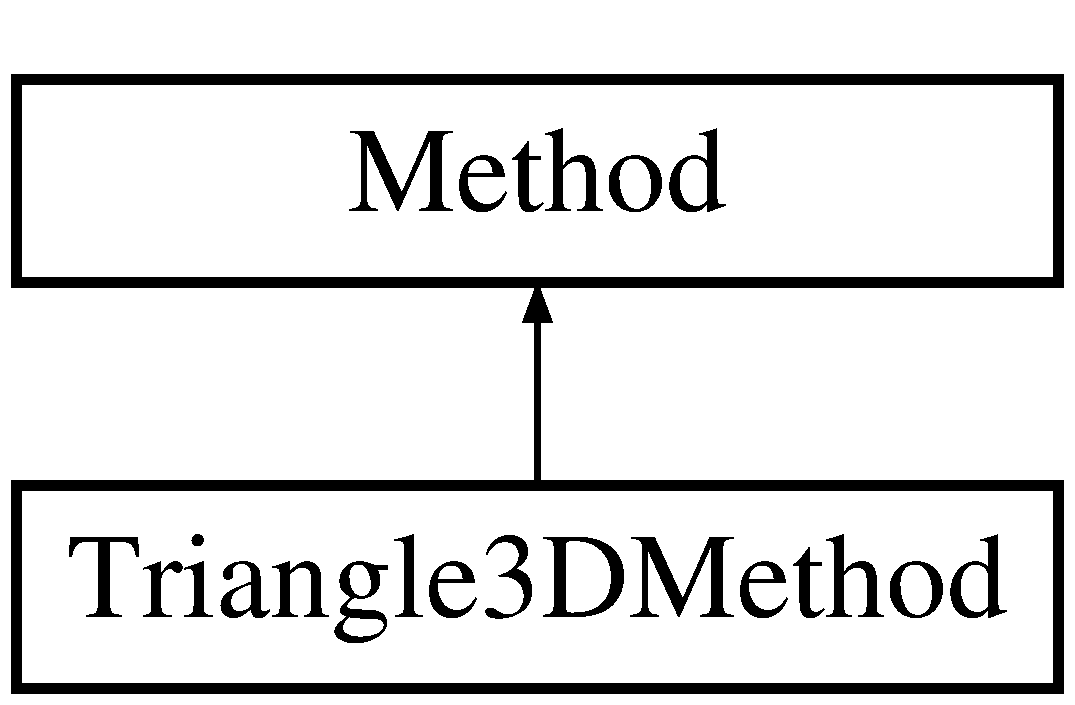
\includegraphics[height=2.000000cm]{classTriangle3DMethod}
\end{center}
\end{figure}
\subsection*{Public Member Functions}
\begin{DoxyCompactItemize}
\item 
\mbox{\Hypertarget{classTriangle3DMethod_aaea704a2e406e58a7cf0e23c95462cc1}\label{classTriangle3DMethod_aaea704a2e406e58a7cf0e23c95462cc1}} 
\hyperlink{classTriangle3DMethod_aaea704a2e406e58a7cf0e23c95462cc1}{Triangle3\+D\+Method} ()
\begin{DoxyCompactList}\small\item\em Constructor. \end{DoxyCompactList}\item 
\mbox{\Hypertarget{classTriangle3DMethod_ae024198c8eb3c4ebb984e191acdf5d83}\label{classTriangle3DMethod_ae024198c8eb3c4ebb984e191acdf5d83}} 
virtual \hyperlink{classTriangle3DMethod_ae024198c8eb3c4ebb984e191acdf5d83}{$\sim$\+Triangle3\+D\+Method} ()
\begin{DoxyCompactList}\small\item\em Descturctor. \end{DoxyCompactList}\item 
virtual void \hyperlink{classTriangle3DMethod_a8e006abc4a38f47bfda0263acfbb7585}{on\+Draw} (glm\+::mat4 const \&proj, glm\+::mat4 const \&view, glm\+::vec3 const \&light, glm\+::vec3 const \&camera) override
\begin{DoxyCompactList}\small\item\em This function is called every frame and should render 3D triangle. \end{DoxyCompactList}\end{DoxyCompactItemize}
\subsection*{Data Fields}
\begin{DoxyCompactItemize}
\item 
\mbox{\Hypertarget{classTriangle3DMethod_a07fddb9a07f2851dd346dc7b449e75c1}\label{classTriangle3DMethod_a07fddb9a07f2851dd346dc7b449e75c1}} 
\hyperlink{fwd_8hpp_a46ffd067c21ab50f5f1fcfed5d8bfc15}{Program\+ID} \hyperlink{classTriangle3DMethod_a07fddb9a07f2851dd346dc7b449e75c1}{prg}
\begin{DoxyCompactList}\small\item\em id of program \end{DoxyCompactList}\item 
\mbox{\Hypertarget{classTriangle3DMethod_ab19d501248c66ebf94b51cf4c2a4aa3c}\label{classTriangle3DMethod_ab19d501248c66ebf94b51cf4c2a4aa3c}} 
\hyperlink{fwd_8hpp_af6f78f73099477c9ce5537d657597486}{Vertex\+Puller\+ID} \hyperlink{classTriangle3DMethod_ab19d501248c66ebf94b51cf4c2a4aa3c}{vao}
\begin{DoxyCompactList}\small\item\em id of vertex puller \end{DoxyCompactList}\end{DoxyCompactItemize}


\subsection{Detailed Description}
This class represents 3D triagnle rendering method. 

\subsection{Member Function Documentation}
\mbox{\Hypertarget{classTriangle3DMethod_a8e006abc4a38f47bfda0263acfbb7585}\label{classTriangle3DMethod_a8e006abc4a38f47bfda0263acfbb7585}} 
\index{Triangle3\+D\+Method@{Triangle3\+D\+Method}!on\+Draw@{on\+Draw}}
\index{on\+Draw@{on\+Draw}!Triangle3\+D\+Method@{Triangle3\+D\+Method}}
\subsubsection{\texorpdfstring{on\+Draw()}{onDraw()}}
{\footnotesize\ttfamily void Triangle3\+D\+Method\+::on\+Draw (\begin{DoxyParamCaption}\item[{glm\+::mat4 const \&}]{proj,  }\item[{glm\+::mat4 const \&}]{view,  }\item[{glm\+::vec3 const \&}]{light,  }\item[{glm\+::vec3 const \&}]{camera }\end{DoxyParamCaption})\hspace{0.3cm}{\ttfamily [override]}, {\ttfamily [virtual]}}



This function is called every frame and should render 3D triangle. 


\begin{DoxyParams}{Parameters}
{\em proj} & projection matrix \\
\hline
{\em view} & view matrix \\
\hline
{\em light} & light position \\
\hline
{\em camera} & camera position \\
\hline
\end{DoxyParams}


Implements \hyperlink{classMethod_ab07a971e2a1b04a658467c643423c347}{Method}.



The documentation for this class was generated from the following files\+:\begin{DoxyCompactItemize}
\item 
student/\hyperlink{triangle3DMethod_8hpp}{triangle3\+D\+Method.\+hpp}\item 
student/\hyperlink{triangle3DMethod_8cpp}{triangle3\+D\+Method.\+cpp}\end{DoxyCompactItemize}

\hypertarget{classTriangleBufferMethod}{}\section{Triangle\+Buffer\+Method Class Reference}
\label{classTriangleBufferMethod}\index{Triangle\+Buffer\+Method@{Triangle\+Buffer\+Method}}


This class represents triangle buffer rendering method.  




{\ttfamily \#include $<$triangle\+Buffer\+Method.\+hpp$>$}

Inheritance diagram for Triangle\+Buffer\+Method\+:\begin{figure}[H]
\begin{center}
\leavevmode
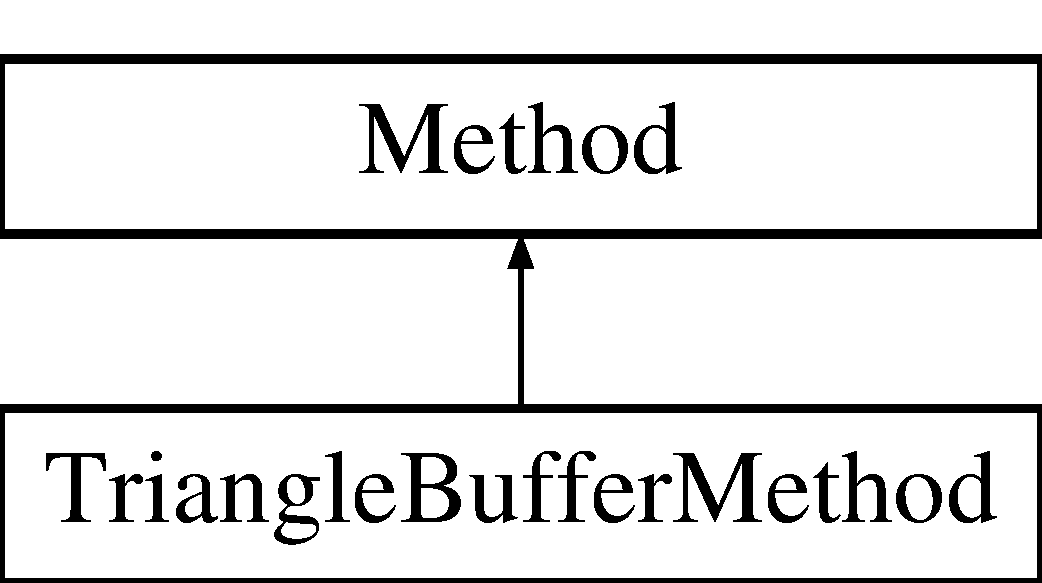
\includegraphics[height=2.000000cm]{classTriangleBufferMethod}
\end{center}
\end{figure}
\subsection*{Public Member Functions}
\begin{DoxyCompactItemize}
\item 
virtual void \hyperlink{classTriangleBufferMethod_ae4339a5479f2f4fe9ca5964d5f7f1f74}{on\+Draw} (glm\+::mat4 const \&proj, glm\+::mat4 const \&view, glm\+::vec3 const \&light, glm\+::vec3 const \&camera) override
\begin{DoxyCompactList}\small\item\em This functino is called every frame. \end{DoxyCompactList}\end{DoxyCompactItemize}
\subsection*{Data Fields}
\begin{DoxyCompactItemize}
\item 
\mbox{\Hypertarget{classTriangleBufferMethod_a692dd8c164b3116b965edceb5792f428}\label{classTriangleBufferMethod_a692dd8c164b3116b965edceb5792f428}} 
\hyperlink{fwd_8hpp_a46ffd067c21ab50f5f1fcfed5d8bfc15}{Program\+ID} \hyperlink{classTriangleBufferMethod_a692dd8c164b3116b965edceb5792f428}{prg}
\begin{DoxyCompactList}\small\item\em id of program \end{DoxyCompactList}\item 
\mbox{\Hypertarget{classTriangleBufferMethod_a26520fbbc3ddf936a2d61d2bf0d9f1fd}\label{classTriangleBufferMethod_a26520fbbc3ddf936a2d61d2bf0d9f1fd}} 
\hyperlink{fwd_8hpp_af6f78f73099477c9ce5537d657597486}{Vertex\+Puller\+ID} \hyperlink{classTriangleBufferMethod_a26520fbbc3ddf936a2d61d2bf0d9f1fd}{vao}
\begin{DoxyCompactList}\small\item\em id of vertex puller \end{DoxyCompactList}\item 
\mbox{\Hypertarget{classTriangleBufferMethod_a5426e29ed114e5e53f35e3a439e11d7d}\label{classTriangleBufferMethod_a5426e29ed114e5e53f35e3a439e11d7d}} 
\hyperlink{fwd_8hpp_a5114031b77b80ad895eff688720b7f93}{Buffer\+ID} \hyperlink{classTriangleBufferMethod_a5426e29ed114e5e53f35e3a439e11d7d}{vbo}
\begin{DoxyCompactList}\small\item\em vertex buffer \end{DoxyCompactList}\end{DoxyCompactItemize}


\subsection{Detailed Description}
This class represents triangle buffer rendering method. 

\subsection{Member Function Documentation}
\mbox{\Hypertarget{classTriangleBufferMethod_ae4339a5479f2f4fe9ca5964d5f7f1f74}\label{classTriangleBufferMethod_ae4339a5479f2f4fe9ca5964d5f7f1f74}} 
\index{Triangle\+Buffer\+Method@{Triangle\+Buffer\+Method}!on\+Draw@{on\+Draw}}
\index{on\+Draw@{on\+Draw}!Triangle\+Buffer\+Method@{Triangle\+Buffer\+Method}}
\subsubsection{\texorpdfstring{on\+Draw()}{onDraw()}}
{\footnotesize\ttfamily void Triangle\+Buffer\+Method\+::on\+Draw (\begin{DoxyParamCaption}\item[{glm\+::mat4 const \&}]{proj,  }\item[{glm\+::mat4 const \&}]{view,  }\item[{glm\+::vec3 const \&}]{light,  }\item[{glm\+::vec3 const \&}]{camera }\end{DoxyParamCaption})\hspace{0.3cm}{\ttfamily [override]}, {\ttfamily [virtual]}}



This functino is called every frame. 


\begin{DoxyParams}{Parameters}
{\em proj} & projection matrix \\
\hline
{\em view} & view matrix \\
\hline
{\em light} & light position \\
\hline
{\em camera} & camera position \\
\hline
\end{DoxyParams}


Implements \hyperlink{classMethod_ab07a971e2a1b04a658467c643423c347}{Method}.



The documentation for this class was generated from the following files\+:\begin{DoxyCompactItemize}
\item 
student/\hyperlink{triangleBufferMethod_8hpp}{triangle\+Buffer\+Method.\+hpp}\item 
student/\hyperlink{triangleBufferMethod_8cpp}{triangle\+Buffer\+Method.\+cpp}\end{DoxyCompactItemize}

\hypertarget{classTriangleClip1Method}{}\section{Triangle\+Clip1\+Method Class Reference}
\label{classTriangleClip1Method}\index{Triangle\+Clip1\+Method@{Triangle\+Clip1\+Method}}


Triangle clipping method 1.  




{\ttfamily \#include $<$triangle\+Clip1\+Method.\+hpp$>$}

Inheritance diagram for Triangle\+Clip1\+Method\+:\begin{figure}[H]
\begin{center}
\leavevmode
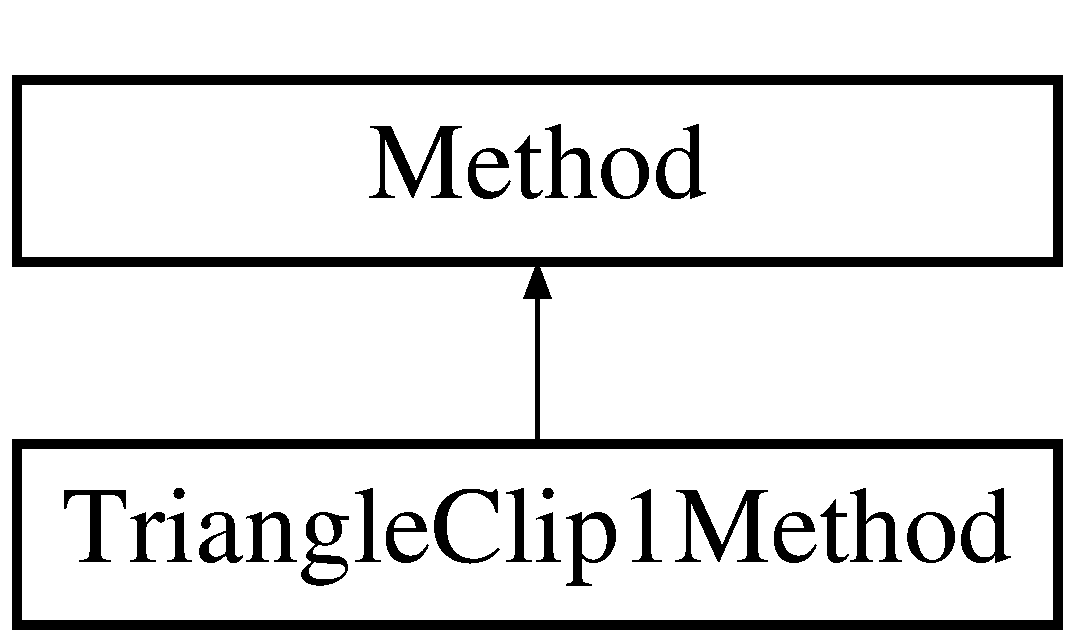
\includegraphics[height=2.000000cm]{classTriangleClip1Method}
\end{center}
\end{figure}
\subsection*{Public Member Functions}
\begin{DoxyCompactItemize}
\item 
virtual void \hyperlink{classTriangleClip1Method_a5761d061239fbd8afa2e8c29cc3bef04}{on\+Draw} (glm\+::mat4 const \&proj, glm\+::mat4 const \&view, glm\+::vec3 const \&light, glm\+::vec3 const \&camera) override
\begin{DoxyCompactList}\small\item\em This functino is called every frame. \end{DoxyCompactList}\end{DoxyCompactItemize}
\subsection*{Data Fields}
\begin{DoxyCompactItemize}
\item 
\mbox{\Hypertarget{classTriangleClip1Method_aeede025939f3728ae3fd9ef40e42005e}\label{classTriangleClip1Method_aeede025939f3728ae3fd9ef40e42005e}} 
\hyperlink{fwd_8hpp_a46ffd067c21ab50f5f1fcfed5d8bfc15}{Program\+ID} \hyperlink{classTriangleClip1Method_aeede025939f3728ae3fd9ef40e42005e}{prg}
\begin{DoxyCompactList}\small\item\em id of program \end{DoxyCompactList}\item 
\mbox{\Hypertarget{classTriangleClip1Method_a9318f0a9370e44f4c97d38ad583cc3fa}\label{classTriangleClip1Method_a9318f0a9370e44f4c97d38ad583cc3fa}} 
\hyperlink{fwd_8hpp_af6f78f73099477c9ce5537d657597486}{Vertex\+Puller\+ID} \hyperlink{classTriangleClip1Method_a9318f0a9370e44f4c97d38ad583cc3fa}{vao}
\begin{DoxyCompactList}\small\item\em id of vertex puller \end{DoxyCompactList}\end{DoxyCompactItemize}


\subsection{Detailed Description}
Triangle clipping method 1. 

\subsection{Member Function Documentation}
\mbox{\Hypertarget{classTriangleClip1Method_a5761d061239fbd8afa2e8c29cc3bef04}\label{classTriangleClip1Method_a5761d061239fbd8afa2e8c29cc3bef04}} 
\index{Triangle\+Clip1\+Method@{Triangle\+Clip1\+Method}!on\+Draw@{on\+Draw}}
\index{on\+Draw@{on\+Draw}!Triangle\+Clip1\+Method@{Triangle\+Clip1\+Method}}
\subsubsection{\texorpdfstring{on\+Draw()}{onDraw()}}
{\footnotesize\ttfamily void Triangle\+Clip1\+Method\+::on\+Draw (\begin{DoxyParamCaption}\item[{glm\+::mat4 const \&}]{proj,  }\item[{glm\+::mat4 const \&}]{view,  }\item[{glm\+::vec3 const \&}]{light,  }\item[{glm\+::vec3 const \&}]{camera }\end{DoxyParamCaption})\hspace{0.3cm}{\ttfamily [override]}, {\ttfamily [virtual]}}



This functino is called every frame. 


\begin{DoxyParams}{Parameters}
{\em proj} & projection matrix \\
\hline
{\em view} & view matrix \\
\hline
{\em light} & light position \\
\hline
{\em camera} & camera position \\
\hline
\end{DoxyParams}


Implements \hyperlink{classMethod_ab07a971e2a1b04a658467c643423c347}{Method}.



The documentation for this class was generated from the following files\+:\begin{DoxyCompactItemize}
\item 
student/\hyperlink{triangleClip1Method_8hpp}{triangle\+Clip1\+Method.\+hpp}\item 
student/\hyperlink{triangleClip1Method_8cpp}{triangle\+Clip1\+Method.\+cpp}\end{DoxyCompactItemize}

\hypertarget{classTriangleClip2Method}{}\section{Triangle\+Clip2\+Method Class Reference}
\label{classTriangleClip2Method}\index{Triangle\+Clip2\+Method@{Triangle\+Clip2\+Method}}


Triangle clipping 2 rendering method.  




{\ttfamily \#include $<$triangle\+Clip2\+Method.\+hpp$>$}

Inheritance diagram for Triangle\+Clip2\+Method\+:\begin{figure}[H]
\begin{center}
\leavevmode
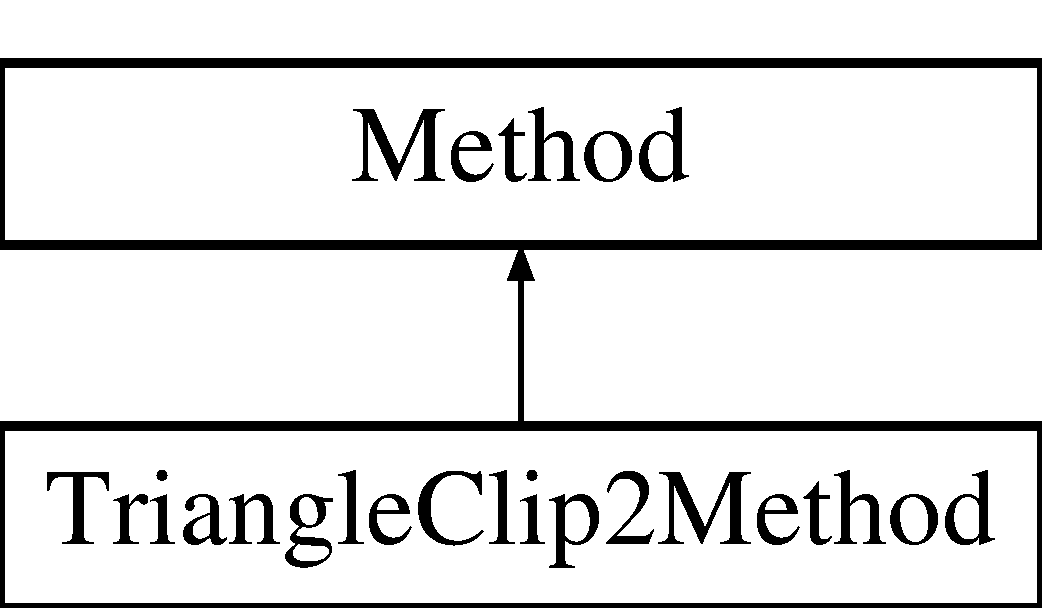
\includegraphics[height=2.000000cm]{classTriangleClip2Method}
\end{center}
\end{figure}
\subsection*{Public Member Functions}
\begin{DoxyCompactItemize}
\item 
virtual void \hyperlink{classTriangleClip2Method_a8433b228a45401ae637ec6d65a047ea5}{on\+Draw} (glm\+::mat4 const \&proj, glm\+::mat4 const \&view, glm\+::vec3 const \&light, glm\+::vec3 const \&camera) override
\begin{DoxyCompactList}\small\item\em This functino is called every frame. \end{DoxyCompactList}\end{DoxyCompactItemize}
\subsection*{Data Fields}
\begin{DoxyCompactItemize}
\item 
\mbox{\Hypertarget{classTriangleClip2Method_a88f7bc73ef771bef04bf03194764ca26}\label{classTriangleClip2Method_a88f7bc73ef771bef04bf03194764ca26}} 
\hyperlink{fwd_8hpp_a46ffd067c21ab50f5f1fcfed5d8bfc15}{Program\+ID} \hyperlink{classTriangleClip2Method_a88f7bc73ef771bef04bf03194764ca26}{prg}
\begin{DoxyCompactList}\small\item\em id of program \end{DoxyCompactList}\item 
\mbox{\Hypertarget{classTriangleClip2Method_a006049aeb1b86f7f94504b0d7b13f4a9}\label{classTriangleClip2Method_a006049aeb1b86f7f94504b0d7b13f4a9}} 
\hyperlink{fwd_8hpp_af6f78f73099477c9ce5537d657597486}{Vertex\+Puller\+ID} \hyperlink{classTriangleClip2Method_a006049aeb1b86f7f94504b0d7b13f4a9}{vao}
\begin{DoxyCompactList}\small\item\em id of vertex puller \end{DoxyCompactList}\end{DoxyCompactItemize}


\subsection{Detailed Description}
Triangle clipping 2 rendering method. 

\subsection{Member Function Documentation}
\mbox{\Hypertarget{classTriangleClip2Method_a8433b228a45401ae637ec6d65a047ea5}\label{classTriangleClip2Method_a8433b228a45401ae637ec6d65a047ea5}} 
\index{Triangle\+Clip2\+Method@{Triangle\+Clip2\+Method}!on\+Draw@{on\+Draw}}
\index{on\+Draw@{on\+Draw}!Triangle\+Clip2\+Method@{Triangle\+Clip2\+Method}}
\subsubsection{\texorpdfstring{on\+Draw()}{onDraw()}}
{\footnotesize\ttfamily void Triangle\+Clip2\+Method\+::on\+Draw (\begin{DoxyParamCaption}\item[{glm\+::mat4 const \&}]{proj,  }\item[{glm\+::mat4 const \&}]{view,  }\item[{glm\+::vec3 const \&}]{light,  }\item[{glm\+::vec3 const \&}]{camera }\end{DoxyParamCaption})\hspace{0.3cm}{\ttfamily [override]}, {\ttfamily [virtual]}}



This functino is called every frame. 


\begin{DoxyParams}{Parameters}
{\em proj} & projection matrix \\
\hline
{\em view} & view matrix \\
\hline
{\em light} & light position \\
\hline
{\em camera} & camera position \\
\hline
\end{DoxyParams}


Implements \hyperlink{classMethod_ab07a971e2a1b04a658467c643423c347}{Method}.



The documentation for this class was generated from the following files\+:\begin{DoxyCompactItemize}
\item 
student/\hyperlink{triangleClip2Method_8hpp}{triangle\+Clip2\+Method.\+hpp}\item 
student/triangle\+Clip2\+Method.\+cpp\end{DoxyCompactItemize}

\hypertarget{classTriangleMethod}{}\section{Triangle\+Method Class Reference}
\label{classTriangleMethod}\index{Triangle\+Method@{Triangle\+Method}}


2D Triangle rendering method  




{\ttfamily \#include $<$triangle\+Method.\+hpp$>$}

Inheritance diagram for Triangle\+Method\+:\begin{figure}[H]
\begin{center}
\leavevmode
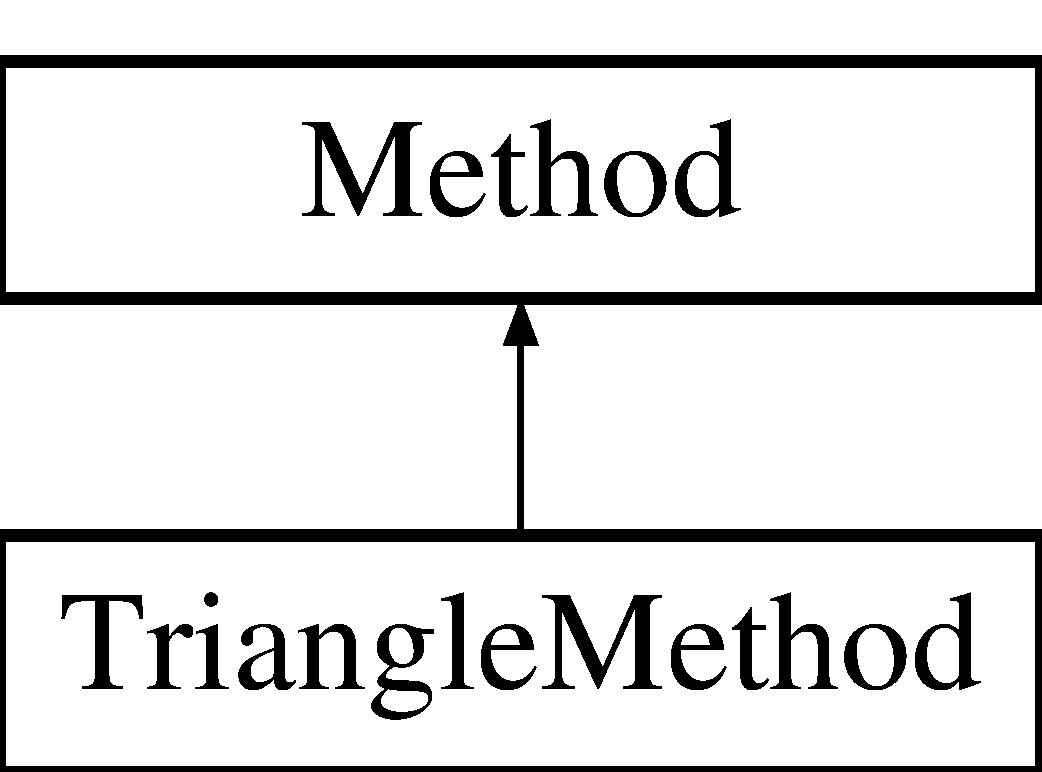
\includegraphics[height=2.000000cm]{classTriangleMethod}
\end{center}
\end{figure}
\subsection*{Public Member Functions}
\begin{DoxyCompactItemize}
\item 
virtual void \hyperlink{classTriangleMethod_a92fa9c2070469055edee05594a8639c9}{on\+Draw} (glm\+::mat4 const \&proj, glm\+::mat4 const \&view, glm\+::vec3 const \&light, glm\+::vec3 const \&camera) override
\begin{DoxyCompactList}\small\item\em This functino is called every frame. \end{DoxyCompactList}\end{DoxyCompactItemize}
\subsection*{Data Fields}
\begin{DoxyCompactItemize}
\item 
\mbox{\Hypertarget{classTriangleMethod_afe56337e65b4f2b2e81c236274ea1e81}\label{classTriangleMethod_afe56337e65b4f2b2e81c236274ea1e81}} 
\hyperlink{fwd_8hpp_a46ffd067c21ab50f5f1fcfed5d8bfc15}{Program\+ID} \hyperlink{classTriangleMethod_afe56337e65b4f2b2e81c236274ea1e81}{prg}
\begin{DoxyCompactList}\small\item\em id of program \end{DoxyCompactList}\item 
\mbox{\Hypertarget{classTriangleMethod_a24b12b7de04a0acd1148632f6d1f1ec3}\label{classTriangleMethod_a24b12b7de04a0acd1148632f6d1f1ec3}} 
\hyperlink{fwd_8hpp_af6f78f73099477c9ce5537d657597486}{Vertex\+Puller\+ID} \hyperlink{classTriangleMethod_a24b12b7de04a0acd1148632f6d1f1ec3}{vao}
\begin{DoxyCompactList}\small\item\em id of vertex puller \end{DoxyCompactList}\end{DoxyCompactItemize}


\subsection{Detailed Description}
2D Triangle rendering method 

\subsection{Member Function Documentation}
\mbox{\Hypertarget{classTriangleMethod_a92fa9c2070469055edee05594a8639c9}\label{classTriangleMethod_a92fa9c2070469055edee05594a8639c9}} 
\index{Triangle\+Method@{Triangle\+Method}!on\+Draw@{on\+Draw}}
\index{on\+Draw@{on\+Draw}!Triangle\+Method@{Triangle\+Method}}
\subsubsection{\texorpdfstring{on\+Draw()}{onDraw()}}
{\footnotesize\ttfamily void Triangle\+Method\+::on\+Draw (\begin{DoxyParamCaption}\item[{glm\+::mat4 const \&}]{proj,  }\item[{glm\+::mat4 const \&}]{view,  }\item[{glm\+::vec3 const \&}]{light,  }\item[{glm\+::vec3 const \&}]{camera }\end{DoxyParamCaption})\hspace{0.3cm}{\ttfamily [override]}, {\ttfamily [virtual]}}



This functino is called every frame. 


\begin{DoxyParams}{Parameters}
{\em proj} & projection matrix \\
\hline
{\em view} & view matrix \\
\hline
{\em light} & light position \\
\hline
{\em camera} & camera position \\
\hline
\end{DoxyParams}


Implements \hyperlink{classMethod_ab07a971e2a1b04a658467c643423c347}{Method}.



The documentation for this class was generated from the following files\+:\begin{DoxyCompactItemize}
\item 
student/\hyperlink{triangleMethod_8hpp}{triangle\+Method.\+hpp}\item 
student/\hyperlink{triangleMethod_8cpp}{triangle\+Method.\+cpp}\end{DoxyCompactItemize}

\hypertarget{unionUniform}{}\section{Uniform Union Reference}
\label{unionUniform}\index{Uniform@{Uniform}}


This union represents one uniform variable.  




{\ttfamily \#include $<$fwd.\+hpp$>$}

\subsection*{Data Fields}
\begin{DoxyCompactItemize}
\item 
\mbox{\Hypertarget{unionUniform_a2714f4ff3e6703bccdac2c92dcad3b25}\label{unionUniform_a2714f4ff3e6703bccdac2c92dcad3b25}} 
float \hyperlink{unionUniform_a2714f4ff3e6703bccdac2c92dcad3b25}{v1}
\begin{DoxyCompactList}\small\item\em single float \end{DoxyCompactList}\item 
\mbox{\Hypertarget{unionUniform_ae497d8a71600e5eb222cbcf8ad71788f}\label{unionUniform_ae497d8a71600e5eb222cbcf8ad71788f}} 
glm\+::vec2 \hyperlink{unionUniform_ae497d8a71600e5eb222cbcf8ad71788f}{v2}
\begin{DoxyCompactList}\small\item\em two floats \end{DoxyCompactList}\item 
\mbox{\Hypertarget{unionUniform_a70392e438c775c6213e6c2dec76b29c4}\label{unionUniform_a70392e438c775c6213e6c2dec76b29c4}} 
glm\+::vec3 \hyperlink{unionUniform_a70392e438c775c6213e6c2dec76b29c4}{v3}
\begin{DoxyCompactList}\small\item\em three floats \end{DoxyCompactList}\item 
\mbox{\Hypertarget{unionUniform_ad2afb58e290202cd23e444440e1b1f07}\label{unionUniform_ad2afb58e290202cd23e444440e1b1f07}} 
glm\+::vec4 \hyperlink{unionUniform_ad2afb58e290202cd23e444440e1b1f07}{v4}
\begin{DoxyCompactList}\small\item\em four floats \end{DoxyCompactList}\item 
\mbox{\Hypertarget{unionUniform_aec09b95ed538f79020d6e70323b27771}\label{unionUniform_aec09b95ed538f79020d6e70323b27771}} 
glm\+::mat4 \hyperlink{unionUniform_aec09b95ed538f79020d6e70323b27771}{m4} = glm\+::mat4(1.f)
\begin{DoxyCompactList}\small\item\em 4x4 float matrix \end{DoxyCompactList}\end{DoxyCompactItemize}


\subsection{Detailed Description}
This union represents one uniform variable. 

The documentation for this union was generated from the following file\+:\begin{DoxyCompactItemize}
\item 
student/\hyperlink{fwd_8hpp}{fwd.\+hpp}\end{DoxyCompactItemize}

\hypertarget{structUniforms}{}\section{Uniforms Struct Reference}
\label{structUniforms}\index{Uniforms@{Uniforms}}


This struct represents shader program uniform variables.  




{\ttfamily \#include $<$fwd.\+hpp$>$}

\subsection*{Data Fields}
\begin{DoxyCompactItemize}
\item 
\mbox{\Hypertarget{structUniforms_ac1130b74094bf1d7eaa9e18b332deff9}\label{structUniforms_ac1130b74094bf1d7eaa9e18b332deff9}} 
\hyperlink{unionUniform}{Uniform} \hyperlink{structUniforms_ac1130b74094bf1d7eaa9e18b332deff9}{uniform} \mbox{[}\hyperlink{fwd_8hpp_abb316cce98ea6938a7112c5f932d673f}{max\+Uniforms}\mbox{]}
\begin{DoxyCompactList}\small\item\em uniform variables \end{DoxyCompactList}\end{DoxyCompactItemize}


\subsection{Detailed Description}
This struct represents shader program uniform variables. 

The documentation for this struct was generated from the following file\+:\begin{DoxyCompactItemize}
\item 
student/\hyperlink{fwd_8hpp}{fwd.\+hpp}\end{DoxyCompactItemize}

\hypertarget{classWindow}{}\section{Window Class Reference}
\label{classWindow}\index{Window@{Window}}


This class represents S\+DL window.  




{\ttfamily \#include $<$window.\+hpp$>$}

Inheritance diagram for Window\+:\begin{figure}[H]
\begin{center}
\leavevmode
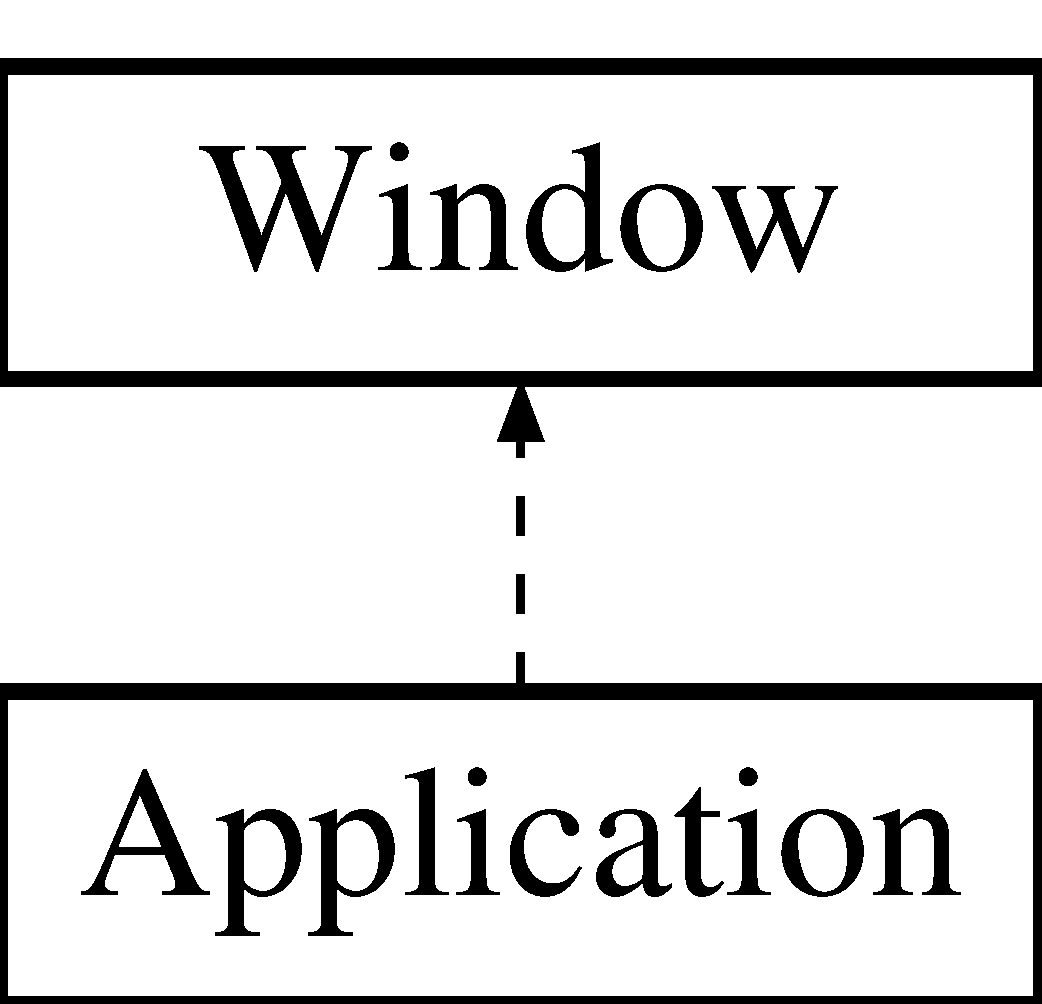
\includegraphics[height=2.000000cm]{classWindow}
\end{center}
\end{figure}
\subsection*{Public Types}
\begin{DoxyCompactItemize}
\item 
\mbox{\Hypertarget{classWindow_a0e7a1332f3c35705eeed4d7b1a568d61}\label{classWindow_a0e7a1332f3c35705eeed4d7b1a568d61}} 
using \hyperlink{classWindow_a0e7a1332f3c35705eeed4d7b1a568d61}{Event\+Callback} = std\+::function$<$ void(S\+D\+L\+\_\+\+Event const  \&e)$>$
\begin{DoxyCompactList}\small\item\em Type of event callback function. \end{DoxyCompactList}\item 
\mbox{\Hypertarget{classWindow_ae666e38583ffdec789fdfc85d6504d73}\label{classWindow_ae666e38583ffdec789fdfc85d6504d73}} 
using \hyperlink{classWindow_ae666e38583ffdec789fdfc85d6504d73}{Idle\+Callback} = std\+::function$<$ void()$>$
\begin{DoxyCompactList}\small\item\em Type of idle callback function. \end{DoxyCompactList}\end{DoxyCompactItemize}
\subsection*{Public Member Functions}
\begin{DoxyCompactItemize}
\item 
\hyperlink{classWindow_ac84f7bfb1b67b73c69a582fe72339192}{Window} (int32\+\_\+t width, int32\+\_\+t height, char const $\ast$name)
\begin{DoxyCompactList}\small\item\em Constructor of \hyperlink{classWindow}{Window} instance. \end{DoxyCompactList}\item 
\mbox{\Hypertarget{classWindow_a245d821e6016fa1f6970ccbbedd635f6}\label{classWindow_a245d821e6016fa1f6970ccbbedd635f6}} 
virtual \hyperlink{classWindow_a245d821e6016fa1f6970ccbbedd635f6}{$\sim$\+Window} ()
\begin{DoxyCompactList}\small\item\em Destructor of \hyperlink{classWindow}{Window} instance. \end{DoxyCompactList}\item 
\mbox{\Hypertarget{classWindow_a4e50cfd8622784e15409db62d5e11097}\label{classWindow_a4e50cfd8622784e15409db62d5e11097}} 
void \hyperlink{classWindow_a4e50cfd8622784e15409db62d5e11097}{main\+Loop} ()
\begin{DoxyCompactList}\small\item\em This is the main loop of the window. \end{DoxyCompactList}\item 
void \hyperlink{classWindow_a10bc693cad6ea33409071ed50c3e880c}{set\+Callback} (uint32\+\_\+t event, \hyperlink{classWindow_a0e7a1332f3c35705eeed4d7b1a568d61}{Event\+Callback} const \&clb)
\begin{DoxyCompactList}\small\item\em This function sets callback for event. \end{DoxyCompactList}\item 
void \hyperlink{classWindow_a4cc4f07c386516c8607bfc7559319112}{set\+Window\+Callback} (uint32\+\_\+t event, \hyperlink{classWindow_a0e7a1332f3c35705eeed4d7b1a568d61}{Event\+Callback} const \&clb)
\begin{DoxyCompactList}\small\item\em This function sets window callback. \end{DoxyCompactList}\item 
void \hyperlink{classWindow_ac1cd27329e92882a1527eece8aa4bef4}{set\+Idle\+Callback} (\hyperlink{classWindow_ae666e38583ffdec789fdfc85d6504d73}{Idle\+Callback} const \&clb)
\begin{DoxyCompactList}\small\item\em This function sets idle callback -\/ function that is called when there are not events. \end{DoxyCompactList}\item 
\mbox{\Hypertarget{classWindow_a383e6781d7d6ae31ebbd8a4cc0df88da}\label{classWindow_a383e6781d7d6ae31ebbd8a4cc0df88da}} 
void \hyperlink{classWindow_a383e6781d7d6ae31ebbd8a4cc0df88da}{re\+Init\+Renderer} ()
\begin{DoxyCompactList}\small\item\em This function reinits S\+DL renderer. \end{DoxyCompactList}\item 
S\+D\+L\+\_\+\+Window $\ast$ \hyperlink{classWindow_a248f74edd46fe00cb6a2c93bd048c26f}{get\+Window} ()
\begin{DoxyCompactList}\small\item\em This function returns S\+DL window handle. \end{DoxyCompactList}\end{DoxyCompactItemize}
\subsection*{Protected Member Functions}
\begin{DoxyCompactItemize}
\item 
\mbox{\Hypertarget{classWindow_a99e0671f31b1e0fae2309dfbe8d54daf}\label{classWindow_a99e0671f31b1e0fae2309dfbe8d54daf}} 
void \hyperlink{classWindow_a99e0671f31b1e0fae2309dfbe8d54daf}{init\+S\+DL} ()
\begin{DoxyCompactList}\small\item\em This function initializes S\+DL. \end{DoxyCompactList}\item 
void \hyperlink{classWindow_a520e7a72c81aa1bf3b8d7e4b59906569}{init\+Window} (int32\+\_\+t width, int32\+\_\+t height, char const $\ast$name)
\begin{DoxyCompactList}\small\item\em This funciton initialized S\+DL window. \end{DoxyCompactList}\item 
\mbox{\Hypertarget{classWindow_a505288fdd1cf4ae5e6f781260e257fce}\label{classWindow_a505288fdd1cf4ae5e6f781260e257fce}} 
void \hyperlink{classWindow_a505288fdd1cf4ae5e6f781260e257fce}{init\+Surface} ()
\begin{DoxyCompactList}\small\item\em This function initializes S\+DL surface. \end{DoxyCompactList}\item 
\mbox{\Hypertarget{classWindow_acc6425810e18a85137aa70a8c5d11f97}\label{classWindow_acc6425810e18a85137aa70a8c5d11f97}} 
void \hyperlink{classWindow_acc6425810e18a85137aa70a8c5d11f97}{init\+Renderer} ()
\begin{DoxyCompactList}\small\item\em This function inzializes S\+DL renderer. \end{DoxyCompactList}\item 
\mbox{\Hypertarget{classWindow_af21aa4f51374ee5234701e4b122950d8}\label{classWindow_af21aa4f51374ee5234701e4b122950d8}} 
void \hyperlink{classWindow_af21aa4f51374ee5234701e4b122950d8}{init\+Events} ()
\begin{DoxyCompactList}\small\item\em This function initializes S\+DL vents. \end{DoxyCompactList}\item 
\mbox{\Hypertarget{classWindow_a381364c2704bed978cdf9df669c4b629}\label{classWindow_a381364c2704bed978cdf9df669c4b629}} 
void \hyperlink{classWindow_a381364c2704bed978cdf9df669c4b629}{process\+Events} ()
\begin{DoxyCompactList}\small\item\em This function processes all S\+DL eents. \end{DoxyCompactList}\item 
void \hyperlink{classWindow_a31e1886b2016544baa55bedcc4f3b48b}{process\+Event} (S\+D\+L\+\_\+\+Event const \&event)
\begin{DoxyCompactList}\small\item\em This funciton processes one S\+DL event. \end{DoxyCompactList}\item 
void \hyperlink{classWindow_a65c68d5dc2ebc68108662978e86efd25}{process\+Window\+Event} (S\+D\+L\+\_\+\+Event const \&event)
\begin{DoxyCompactList}\small\item\em This function processes one S\+DL window event. \end{DoxyCompactList}\item 
\mbox{\Hypertarget{classWindow_a4a94fbab09672f8360e855ac9ba3becb}\label{classWindow_a4a94fbab09672f8360e855ac9ba3becb}} 
void \hyperlink{classWindow_a4a94fbab09672f8360e855ac9ba3becb}{call\+Idle\+Callback} ()
\begin{DoxyCompactList}\small\item\em This function calls user defined idle callback. \end{DoxyCompactList}\end{DoxyCompactItemize}
\subsection*{Protected Attributes}
\begin{DoxyCompactItemize}
\item 
\mbox{\Hypertarget{classWindow_ae39a7755a5a6ab74bcbdbe3e2e206820}\label{classWindow_ae39a7755a5a6ab74bcbdbe3e2e206820}} 
S\+D\+L\+\_\+\+Window $\ast$ \hyperlink{classWindow_ae39a7755a5a6ab74bcbdbe3e2e206820}{window}
\begin{DoxyCompactList}\small\item\em window handle \end{DoxyCompactList}\item 
\mbox{\Hypertarget{classWindow_a1a42da4979d383bb3556f62df57952e5}\label{classWindow_a1a42da4979d383bb3556f62df57952e5}} 
S\+D\+L\+\_\+\+Surface $\ast$ \hyperlink{classWindow_a1a42da4979d383bb3556f62df57952e5}{surface}
\begin{DoxyCompactList}\small\item\em surface \end{DoxyCompactList}\item 
\mbox{\Hypertarget{classWindow_a2b52309ef359b6392454a3bb57398b5d}\label{classWindow_a2b52309ef359b6392454a3bb57398b5d}} 
S\+D\+L\+\_\+\+Renderer $\ast$ \hyperlink{classWindow_a2b52309ef359b6392454a3bb57398b5d}{renderer}
\begin{DoxyCompactList}\small\item\em S\+D\+L2 renderer. \end{DoxyCompactList}\item 
\mbox{\Hypertarget{classWindow_a3a4074a228d183644d5bb379ceb137f6}\label{classWindow_a3a4074a228d183644d5bb379ceb137f6}} 
bool \hyperlink{classWindow_a3a4074a228d183644d5bb379ceb137f6}{running}
\begin{DoxyCompactList}\small\item\em is main loop running \end{DoxyCompactList}\item 
\mbox{\Hypertarget{classWindow_ae109ff1ae7efd24eb863a87435c230b9}\label{classWindow_ae109ff1ae7efd24eb863a87435c230b9}} 
std\+::map$<$ Uint32, \hyperlink{classWindow_a0e7a1332f3c35705eeed4d7b1a568d61}{Event\+Callback} $>$ \hyperlink{classWindow_ae109ff1ae7efd24eb863a87435c230b9}{event\+Callbacks}
\begin{DoxyCompactList}\small\item\em map of event callback function \end{DoxyCompactList}\item 
\mbox{\Hypertarget{classWindow_a559418e04c7331f18d899f0570416631}\label{classWindow_a559418e04c7331f18d899f0570416631}} 
std\+::map$<$ Uint8,\hyperlink{classWindow_a0e7a1332f3c35705eeed4d7b1a568d61}{Event\+Callback} $>$ \hyperlink{classWindow_a559418e04c7331f18d899f0570416631}{window\+Callbacks}
\begin{DoxyCompactList}\small\item\em map of event callback function for window event \end{DoxyCompactList}\item 
\mbox{\Hypertarget{classWindow_aca8fcf0113fd079f5bc4050c1f72a93b}\label{classWindow_aca8fcf0113fd079f5bc4050c1f72a93b}} 
\hyperlink{classWindow_ae666e38583ffdec789fdfc85d6504d73}{Idle\+Callback} \hyperlink{classWindow_aca8fcf0113fd079f5bc4050c1f72a93b}{idle\+Callback}
\begin{DoxyCompactList}\small\item\em function that is called in mainloop when there are no events \end{DoxyCompactList}\end{DoxyCompactItemize}


\subsection{Detailed Description}
This class represents S\+DL window. 

\subsection{Constructor \& Destructor Documentation}
\mbox{\Hypertarget{classWindow_ac84f7bfb1b67b73c69a582fe72339192}\label{classWindow_ac84f7bfb1b67b73c69a582fe72339192}} 
\index{Window@{Window}!Window@{Window}}
\index{Window@{Window}!Window@{Window}}
\subsubsection{\texorpdfstring{Window()}{Window()}}
{\footnotesize\ttfamily Window\+::\+Window (\begin{DoxyParamCaption}\item[{int32\+\_\+t}]{width,  }\item[{int32\+\_\+t}]{height,  }\item[{char const $\ast$}]{name }\end{DoxyParamCaption})}



Constructor of \hyperlink{classWindow}{Window} instance. 


\begin{DoxyParams}{Parameters}
{\em width} & width of the window \\
\hline
{\em height} & height of the window \\
\hline
{\em name} & name of the window \\
\hline
\end{DoxyParams}


\subsection{Member Function Documentation}
\mbox{\Hypertarget{classWindow_a248f74edd46fe00cb6a2c93bd048c26f}\label{classWindow_a248f74edd46fe00cb6a2c93bd048c26f}} 
\index{Window@{Window}!get\+Window@{get\+Window}}
\index{get\+Window@{get\+Window}!Window@{Window}}
\subsubsection{\texorpdfstring{get\+Window()}{getWindow()}}
{\footnotesize\ttfamily S\+D\+L\+\_\+\+Window $\ast$ Window\+::get\+Window (\begin{DoxyParamCaption}{ }\end{DoxyParamCaption})}



This function returns S\+DL window handle. 

\begin{DoxyReturn}{Returns}
S\+DL window handle 
\end{DoxyReturn}
\mbox{\Hypertarget{classWindow_a520e7a72c81aa1bf3b8d7e4b59906569}\label{classWindow_a520e7a72c81aa1bf3b8d7e4b59906569}} 
\index{Window@{Window}!init\+Window@{init\+Window}}
\index{init\+Window@{init\+Window}!Window@{Window}}
\subsubsection{\texorpdfstring{init\+Window()}{initWindow()}}
{\footnotesize\ttfamily void Window\+::init\+Window (\begin{DoxyParamCaption}\item[{int32\+\_\+t}]{width,  }\item[{int32\+\_\+t}]{height,  }\item[{char const $\ast$}]{name }\end{DoxyParamCaption})\hspace{0.3cm}{\ttfamily [protected]}}



This funciton initialized S\+DL window. 


\begin{DoxyParams}{Parameters}
{\em width} & width of the window \\
\hline
{\em height} & height of the window \\
\hline
{\em name} & name of the window \\
\hline
\end{DoxyParams}
\mbox{\Hypertarget{classWindow_a31e1886b2016544baa55bedcc4f3b48b}\label{classWindow_a31e1886b2016544baa55bedcc4f3b48b}} 
\index{Window@{Window}!process\+Event@{process\+Event}}
\index{process\+Event@{process\+Event}!Window@{Window}}
\subsubsection{\texorpdfstring{process\+Event()}{processEvent()}}
{\footnotesize\ttfamily void Window\+::process\+Event (\begin{DoxyParamCaption}\item[{S\+D\+L\+\_\+\+Event const \&}]{event }\end{DoxyParamCaption})\hspace{0.3cm}{\ttfamily [protected]}}



This funciton processes one S\+DL event. 


\begin{DoxyParams}{Parameters}
{\em event} & S\+DL event \\
\hline
\end{DoxyParams}
\mbox{\Hypertarget{classWindow_a65c68d5dc2ebc68108662978e86efd25}\label{classWindow_a65c68d5dc2ebc68108662978e86efd25}} 
\index{Window@{Window}!process\+Window\+Event@{process\+Window\+Event}}
\index{process\+Window\+Event@{process\+Window\+Event}!Window@{Window}}
\subsubsection{\texorpdfstring{process\+Window\+Event()}{processWindowEvent()}}
{\footnotesize\ttfamily void Window\+::process\+Window\+Event (\begin{DoxyParamCaption}\item[{S\+D\+L\+\_\+\+Event const \&}]{event }\end{DoxyParamCaption})\hspace{0.3cm}{\ttfamily [protected]}}



This function processes one S\+DL window event. 


\begin{DoxyParams}{Parameters}
{\em event} & S\+DL event \\
\hline
\end{DoxyParams}
\mbox{\Hypertarget{classWindow_a10bc693cad6ea33409071ed50c3e880c}\label{classWindow_a10bc693cad6ea33409071ed50c3e880c}} 
\index{Window@{Window}!set\+Callback@{set\+Callback}}
\index{set\+Callback@{set\+Callback}!Window@{Window}}
\subsubsection{\texorpdfstring{set\+Callback()}{setCallback()}}
{\footnotesize\ttfamily void Window\+::set\+Callback (\begin{DoxyParamCaption}\item[{uint32\+\_\+t}]{event,  }\item[{\hyperlink{classWindow_a0e7a1332f3c35705eeed4d7b1a568d61}{Event\+Callback} const \&}]{clb }\end{DoxyParamCaption})}



This function sets callback for event. 


\begin{DoxyParams}{Parameters}
{\em event} & event type from S\+DL \\
\hline
{\em clb} & callback \\
\hline
\end{DoxyParams}
\mbox{\Hypertarget{classWindow_ac1cd27329e92882a1527eece8aa4bef4}\label{classWindow_ac1cd27329e92882a1527eece8aa4bef4}} 
\index{Window@{Window}!set\+Idle\+Callback@{set\+Idle\+Callback}}
\index{set\+Idle\+Callback@{set\+Idle\+Callback}!Window@{Window}}
\subsubsection{\texorpdfstring{set\+Idle\+Callback()}{setIdleCallback()}}
{\footnotesize\ttfamily void Window\+::set\+Idle\+Callback (\begin{DoxyParamCaption}\item[{\hyperlink{classWindow_ae666e38583ffdec789fdfc85d6504d73}{Idle\+Callback} const \&}]{clb }\end{DoxyParamCaption})}



This function sets idle callback -\/ function that is called when there are not events. 


\begin{DoxyParams}{Parameters}
{\em clb} & callback \\
\hline
\end{DoxyParams}
\mbox{\Hypertarget{classWindow_a4cc4f07c386516c8607bfc7559319112}\label{classWindow_a4cc4f07c386516c8607bfc7559319112}} 
\index{Window@{Window}!set\+Window\+Callback@{set\+Window\+Callback}}
\index{set\+Window\+Callback@{set\+Window\+Callback}!Window@{Window}}
\subsubsection{\texorpdfstring{set\+Window\+Callback()}{setWindowCallback()}}
{\footnotesize\ttfamily void Window\+::set\+Window\+Callback (\begin{DoxyParamCaption}\item[{uint32\+\_\+t}]{event,  }\item[{\hyperlink{classWindow_a0e7a1332f3c35705eeed4d7b1a568d61}{Event\+Callback} const \&}]{clb }\end{DoxyParamCaption})}



This function sets window callback. 


\begin{DoxyParams}{Parameters}
{\em event} & window event type from S\+DL \\
\hline
{\em clb} & callback \\
\hline
\end{DoxyParams}


The documentation for this class was generated from the following files\+:\begin{DoxyCompactItemize}
\item 
student/\hyperlink{window_8hpp}{window.\+hpp}\item 
student/\hyperlink{window_8cpp}{window.\+cpp}\end{DoxyCompactItemize}

\chapter{File Documentation}
\hypertarget{application_8cpp}{}\section{student/application.cpp File Reference}
\label{application_8cpp}\index{student/application.\+cpp@{student/application.\+cpp}}


This file contains application class implementation.  


{\ttfamily \#include $<$assert.\+h$>$}\newline
{\ttfamily \#include $<$student/application.\+hpp$>$}\newline
\subsection*{Functions}
\begin{DoxyCompactItemize}
\item 
void \hyperlink{application_8cpp_a93e81d6d69ee21c7500528c70b65bfbc}{copy\+To\+S\+D\+L\+Surface} (S\+D\+L\+\_\+\+Surface $\ast$surface, uint8\+\_\+t const $\ast$const frame, uint32\+\_\+t width, uint32\+\_\+t height)
\begin{DoxyCompactList}\small\item\em This function swaps color buffer with S\+D\+L\+\_\+\+Surface. \end{DoxyCompactList}\end{DoxyCompactItemize}


\subsection{Detailed Description}
This file contains application class implementation. 

\begin{DoxyAuthor}{Author}
Tomáš Milet, \href{mailto:imilet@fit.vutbr.cz}{\tt imilet@fit.\+vutbr.\+cz} 
\end{DoxyAuthor}


\subsection{Function Documentation}
\mbox{\Hypertarget{application_8cpp_a93e81d6d69ee21c7500528c70b65bfbc}\label{application_8cpp_a93e81d6d69ee21c7500528c70b65bfbc}} 
\index{application.\+cpp@{application.\+cpp}!copy\+To\+S\+D\+L\+Surface@{copy\+To\+S\+D\+L\+Surface}}
\index{copy\+To\+S\+D\+L\+Surface@{copy\+To\+S\+D\+L\+Surface}!application.\+cpp@{application.\+cpp}}
\subsubsection{\texorpdfstring{copy\+To\+S\+D\+L\+Surface()}{copyToSDLSurface()}}
{\footnotesize\ttfamily void copy\+To\+S\+D\+L\+Surface (\begin{DoxyParamCaption}\item[{S\+D\+L\+\_\+\+Surface $\ast$}]{surface,  }\item[{uint8\+\_\+t const $\ast$const}]{color,  }\item[{uint32\+\_\+t}]{width,  }\item[{uint32\+\_\+t}]{height }\end{DoxyParamCaption})}



This function swaps color buffer with S\+D\+L\+\_\+\+Surface. 


\begin{DoxyParams}{Parameters}
{\em surface} & sdl surface \\
\hline
{\em color} & color buffer (R\+G\+B\+A8\+UI) \\
\hline
{\em width} & width of color buffer \\
\hline
{\em height} & height of color buffer \\
\hline
\end{DoxyParams}

\hypertarget{application_8hpp}{}\section{student/application.hpp File Reference}
\label{application_8hpp}\index{student/application.\+hpp@{student/application.\+hpp}}


This file contains application class.  


{\ttfamily \#include $<$memory$>$}\newline
{\ttfamily \#include $<$vector$>$}\newline
{\ttfamily \#include $<$Basic\+Camera/\+Orbit\+Camera.\+h$>$}\newline
{\ttfamily \#include $<$Basic\+Camera/\+Perspective\+Camera.\+h$>$}\newline
{\ttfamily \#include $<$student/gpu.\+hpp$>$}\newline
{\ttfamily \#include $<$student/window.\+hpp$>$}\newline
{\ttfamily \#include $<$student/method.\+hpp$>$}\newline
{\ttfamily \#include $<$student/timer.\+hpp$>$}\newline
\subsection*{Data Structures}
\begin{DoxyCompactItemize}
\item 
class \hyperlink{classApplication}{Application}
\begin{DoxyCompactList}\small\item\em \hyperlink{classApplication}{Application} class. \end{DoxyCompactList}\end{DoxyCompactItemize}
\subsection*{Functions}
\begin{DoxyCompactItemize}
\item 
void \hyperlink{application_8hpp_a836867a62b745ce6dad1043f511b010f}{copy\+To\+S\+D\+L\+Surface} (S\+D\+L\+\_\+\+Surface $\ast$surface, uint8\+\_\+t const $\ast$const color, uint32\+\_\+t width, uint32\+\_\+t height)
\begin{DoxyCompactList}\small\item\em This function swaps color buffer with S\+D\+L\+\_\+\+Surface. \end{DoxyCompactList}\end{DoxyCompactItemize}


\subsection{Detailed Description}
This file contains application class. 

\begin{DoxyAuthor}{Author}
Tomáš Milet, \href{mailto:imilet@fit.vutbr.cz}{\tt imilet@fit.\+vutbr.\+cz} 
\end{DoxyAuthor}


\subsection{Function Documentation}
\mbox{\Hypertarget{application_8hpp_a836867a62b745ce6dad1043f511b010f}\label{application_8hpp_a836867a62b745ce6dad1043f511b010f}} 
\index{application.\+hpp@{application.\+hpp}!copy\+To\+S\+D\+L\+Surface@{copy\+To\+S\+D\+L\+Surface}}
\index{copy\+To\+S\+D\+L\+Surface@{copy\+To\+S\+D\+L\+Surface}!application.\+hpp@{application.\+hpp}}
\subsubsection{\texorpdfstring{copy\+To\+S\+D\+L\+Surface()}{copyToSDLSurface()}}
{\footnotesize\ttfamily void copy\+To\+S\+D\+L\+Surface (\begin{DoxyParamCaption}\item[{S\+D\+L\+\_\+\+Surface $\ast$}]{surface,  }\item[{uint8\+\_\+t const $\ast$const}]{color,  }\item[{uint32\+\_\+t}]{width,  }\item[{uint32\+\_\+t}]{height }\end{DoxyParamCaption})}



This function swaps color buffer with S\+D\+L\+\_\+\+Surface. 


\begin{DoxyParams}{Parameters}
{\em surface} & sdl surface \\
\hline
{\em color} & color buffer (R\+G\+B\+A8\+UI) \\
\hline
{\em width} & width of color buffer \\
\hline
{\em height} & height of color buffer \\
\hline
\end{DoxyParams}

\hypertarget{arguments_8hpp}{}\section{student/arguments.hpp File Reference}
\label{arguments_8hpp}\index{student/arguments.\+hpp@{student/arguments.\+hpp}}


This file contains class for command line parsing.  


{\ttfamily \#include $<$Argument\+Viewer/\+Argument\+Viewer.\+h$>$}\newline
{\ttfamily \#include $<$iostream$>$}\newline
{\ttfamily \#include $<$string$>$}\newline
\subsection*{Data Structures}
\begin{DoxyCompactItemize}
\item 
class \hyperlink{classArguments}{Arguments}
\begin{DoxyCompactList}\small\item\em This class parses command line arguments. \end{DoxyCompactList}\end{DoxyCompactItemize}


\subsection{Detailed Description}
This file contains class for command line parsing. 

\begin{DoxyAuthor}{Author}
Tomáš Milet, \href{mailto:imilet@fit.vutbr.cz}{\tt imilet@fit.\+vutbr.\+cz} 
\end{DoxyAuthor}

\hypertarget{bunny_8cpp}{}\section{student/bunny.cpp File Reference}
\label{bunny_8cpp}\index{student/bunny.\+cpp@{student/bunny.\+cpp}}


This file contains model of Standford bunny in static arrays.  


{\ttfamily \#include $<$student/bunny.\+hpp$>$}\newline
\subsection*{Variables}
\begin{DoxyCompactItemize}
\item 
\mbox{\Hypertarget{bunny_8cpp_abc25b346278a6be207f52c8ca1d5f8eb}\label{bunny_8cpp_abc25b346278a6be207f52c8ca1d5f8eb}} 
struct \hyperlink{structBunnyVertex}{Bunny\+Vertex} const \hyperlink{bunny_8cpp_abc25b346278a6be207f52c8ca1d5f8eb}{bunny\+Vertices} \mbox{[}1048\mbox{]}
\begin{DoxyCompactList}\small\item\em This variable contains vertices of Standford bunny. \end{DoxyCompactList}\item 
\mbox{\Hypertarget{bunny_8cpp_a97d66246b26a9f14f0b8f854257318f9}\label{bunny_8cpp_a97d66246b26a9f14f0b8f854257318f9}} 
const \hyperlink{bunny_8hpp_a39b675ae7d335efcd87bafe6a3af3d06}{Vertex\+Index} \hyperlink{bunny_8cpp_a97d66246b26a9f14f0b8f854257318f9}{bunny\+Indices} \mbox{[}2092\mbox{]}\mbox{[}3\mbox{]}
\begin{DoxyCompactList}\small\item\em This variable contains Standford bunny indices. \end{DoxyCompactList}\end{DoxyCompactItemize}


\subsection{Detailed Description}
This file contains model of Standford bunny in static arrays. 

\begin{DoxyAuthor}{Author}
Tomáš Milet, \href{mailto:imilet@fit.vutbr.cz}{\tt imilet@fit.\+vutbr.\+cz} 
\end{DoxyAuthor}

\hypertarget{bunny_8hpp}{}\section{student/bunny.hpp File Reference}
\label{bunny_8hpp}\index{student/bunny.\+hpp@{student/bunny.\+hpp}}


This file contains model of Standford bunny in static arrays.  


{\ttfamily \#include $<$cstdint$>$}\newline
{\ttfamily \#include $<$student/fwd.\+hpp$>$}\newline
\subsection*{Data Structures}
\begin{DoxyCompactItemize}
\item 
struct \hyperlink{structBunnyVertex}{Bunny\+Vertex}
\begin{DoxyCompactList}\small\item\em This structure represents vertex that contains only position and normal. \end{DoxyCompactList}\end{DoxyCompactItemize}
\subsection*{Typedefs}
\begin{DoxyCompactItemize}
\item 
\mbox{\Hypertarget{bunny_8hpp_a39b675ae7d335efcd87bafe6a3af3d06}\label{bunny_8hpp_a39b675ae7d335efcd87bafe6a3af3d06}} 
using \hyperlink{bunny_8hpp_a39b675ae7d335efcd87bafe6a3af3d06}{Vertex\+Index} = uint32\+\_\+t
\begin{DoxyCompactList}\small\item\em type of index \end{DoxyCompactList}\end{DoxyCompactItemize}
\subsection*{Variables}
\begin{DoxyCompactItemize}
\item 
\mbox{\Hypertarget{bunny_8hpp_abc25b346278a6be207f52c8ca1d5f8eb}\label{bunny_8hpp_abc25b346278a6be207f52c8ca1d5f8eb}} 
struct \hyperlink{structBunnyVertex}{Bunny\+Vertex} const \hyperlink{bunny_8hpp_abc25b346278a6be207f52c8ca1d5f8eb}{bunny\+Vertices} \mbox{[}1048\mbox{]}
\begin{DoxyCompactList}\small\item\em This variable contains vertices of Standford bunny. \end{DoxyCompactList}\item 
\mbox{\Hypertarget{bunny_8hpp_a97d66246b26a9f14f0b8f854257318f9}\label{bunny_8hpp_a97d66246b26a9f14f0b8f854257318f9}} 
const \hyperlink{bunny_8hpp_a39b675ae7d335efcd87bafe6a3af3d06}{Vertex\+Index} \hyperlink{bunny_8hpp_a97d66246b26a9f14f0b8f854257318f9}{bunny\+Indices} \mbox{[}2092\mbox{]}\mbox{[}3\mbox{]}
\begin{DoxyCompactList}\small\item\em This variable contains Standford bunny indices. \end{DoxyCompactList}\end{DoxyCompactItemize}


\subsection{Detailed Description}
This file contains model of Standford bunny in static arrays. 

\begin{DoxyAuthor}{Author}
Tomáš Milet, \href{mailto:imilet@fit.vutbr.cz}{\tt imilet@fit.\+vutbr.\+cz} 
\end{DoxyAuthor}

\hypertarget{czFlagMethod_8cpp}{}\section{student/cz\+Flag\+Method.cpp File Reference}
\label{czFlagMethod_8cpp}\index{student/cz\+Flag\+Method.\+cpp@{student/cz\+Flag\+Method.\+cpp}}


This file contains implementation of czech flag rendering method.  


{\ttfamily \#include $<$student/cz\+Flag\+Method.\+hpp$>$}\newline
{\ttfamily \#include $<$vector$>$}\newline
\subsection*{Functions}
\begin{DoxyCompactItemize}
\item 
void \hyperlink{czFlagMethod_8cpp_a787e2577e9bc9e3a1d683e567222c827}{cz\+Flag\+\_\+\+VS} (\hyperlink{structOutVertex}{Out\+Vertex} \&out\+Vertex, \hyperlink{structInVertex}{In\+Vertex} const \&in\+Vertex, \hyperlink{structUniforms}{Uniforms} const \&uniforms)
\begin{DoxyCompactList}\small\item\em Czech flag vertex shader. \end{DoxyCompactList}\item 
void \hyperlink{czFlagMethod_8cpp_a4dce738cae14f12159fee55e2f7487cc}{cz\+Flag\+\_\+\+FS} (\hyperlink{structOutFragment}{Out\+Fragment} \&out\+Fragment, \hyperlink{structInFragment}{In\+Fragment} const \&in\+Fragment, \hyperlink{structUniforms}{Uniforms} const \&uniforms)
\begin{DoxyCompactList}\small\item\em Czech flag fragment shader. \end{DoxyCompactList}\end{DoxyCompactItemize}


\subsection{Detailed Description}
This file contains implementation of czech flag rendering method. 

\begin{DoxyAuthor}{Author}
Tomáš Milet, \href{mailto:imilet@fit.vutbr.cz}{\tt imilet@fit.\+vutbr.\+cz} 
\end{DoxyAuthor}


\subsection{Function Documentation}
\mbox{\Hypertarget{czFlagMethod_8cpp_a4dce738cae14f12159fee55e2f7487cc}\label{czFlagMethod_8cpp_a4dce738cae14f12159fee55e2f7487cc}} 
\index{cz\+Flag\+Method.\+cpp@{cz\+Flag\+Method.\+cpp}!cz\+Flag\+\_\+\+FS@{cz\+Flag\+\_\+\+FS}}
\index{cz\+Flag\+\_\+\+FS@{cz\+Flag\+\_\+\+FS}!cz\+Flag\+Method.\+cpp@{cz\+Flag\+Method.\+cpp}}
\subsubsection{\texorpdfstring{cz\+Flag\+\_\+\+F\+S()}{czFlag\_FS()}}
{\footnotesize\ttfamily void cz\+Flag\+\_\+\+FS (\begin{DoxyParamCaption}\item[{\hyperlink{structOutFragment}{Out\+Fragment} \&}]{out\+Fragment,  }\item[{\hyperlink{structInFragment}{In\+Fragment} const \&}]{in\+Fragment,  }\item[{\hyperlink{structUniforms}{Uniforms} const \&}]{uniforms }\end{DoxyParamCaption})}



Czech flag fragment shader. 


\begin{DoxyParams}{Parameters}
{\em out\+Fragment} & output fragment \\
\hline
{\em in\+Fragment} & input fragment \\
\hline
{\em uniforms} & uniform variables \\
\hline
\end{DoxyParams}
\mbox{\Hypertarget{czFlagMethod_8cpp_a787e2577e9bc9e3a1d683e567222c827}\label{czFlagMethod_8cpp_a787e2577e9bc9e3a1d683e567222c827}} 
\index{cz\+Flag\+Method.\+cpp@{cz\+Flag\+Method.\+cpp}!cz\+Flag\+\_\+\+VS@{cz\+Flag\+\_\+\+VS}}
\index{cz\+Flag\+\_\+\+VS@{cz\+Flag\+\_\+\+VS}!cz\+Flag\+Method.\+cpp@{cz\+Flag\+Method.\+cpp}}
\subsubsection{\texorpdfstring{cz\+Flag\+\_\+\+V\+S()}{czFlag\_VS()}}
{\footnotesize\ttfamily void cz\+Flag\+\_\+\+VS (\begin{DoxyParamCaption}\item[{\hyperlink{structOutVertex}{Out\+Vertex} \&}]{out\+Vertex,  }\item[{\hyperlink{structInVertex}{In\+Vertex} const \&}]{in\+Vertex,  }\item[{\hyperlink{structUniforms}{Uniforms} const \&}]{uniforms }\end{DoxyParamCaption})}



Czech flag vertex shader. 


\begin{DoxyParams}{Parameters}
{\em out\+Vertex} & out vertex \\
\hline
{\em in\+Vertex} & in vertex \\
\hline
{\em uniforms} & uniform variables \\
\hline
\end{DoxyParams}

\hypertarget{czFlagMethod_8hpp}{}\section{student/cz\+Flag\+Method.hpp File Reference}
\label{czFlagMethod_8hpp}\index{student/cz\+Flag\+Method.\+hpp@{student/cz\+Flag\+Method.\+hpp}}


This file contains czech flag rendering method.  


{\ttfamily \#include $<$student/method.\+hpp$>$}\newline
\subsection*{Data Structures}
\begin{DoxyCompactItemize}
\item 
class \hyperlink{classCZFlagMethod}{C\+Z\+Flag\+Method}
\begin{DoxyCompactList}\small\item\em Czech flag rendering method. \end{DoxyCompactList}\end{DoxyCompactItemize}


\subsection{Detailed Description}
This file contains czech flag rendering method. 

\begin{DoxyAuthor}{Author}
Tomáš Milet, \href{mailto:imilet@fit.vutbr.cz}{\tt imilet@fit.\+vutbr.\+cz} 
\end{DoxyAuthor}

\hypertarget{emptyMethod_8hpp}{}\section{student/empty\+Method.hpp File Reference}
\label{emptyMethod_8hpp}\index{student/empty\+Method.\+hpp@{student/empty\+Method.\+hpp}}


This file contains empty rendering method.  


{\ttfamily \#include $<$student/method.\+hpp$>$}\newline
\subsection*{Data Structures}
\begin{DoxyCompactItemize}
\item 
class \hyperlink{classEmptyMethod}{Empty\+Method}
\begin{DoxyCompactList}\small\item\em Empty rendering method. \end{DoxyCompactList}\end{DoxyCompactItemize}


\subsection{Detailed Description}
This file contains empty rendering method. 

\begin{DoxyAuthor}{Author}
Tomáš Milet, \href{mailto:imilet@fit.vutbr.cz}{\tt imilet@fit.\+vutbr.\+cz} 
\end{DoxyAuthor}

\hypertarget{fwd_8hpp}{}\section{student/fwd.hpp File Reference}
\label{fwd_8hpp}\index{student/fwd.\+hpp@{student/fwd.\+hpp}}


This file contains forward declarations and constants.  


{\ttfamily \#include $<$glm/glm.\+hpp$>$}\newline
{\ttfamily \#include $<$cstdint$>$}\newline
\subsection*{Data Structures}
\begin{DoxyCompactItemize}
\item 
union \hyperlink{unionAttribute}{Attribute}
\begin{DoxyCompactList}\small\item\em This union represents one vertex/fragment attribute. \end{DoxyCompactList}\item 
struct \hyperlink{structInVertex}{In\+Vertex}
\begin{DoxyCompactList}\small\item\em This struct represents input vertex of vertex shader. \end{DoxyCompactList}\item 
struct \hyperlink{structOutVertex}{Out\+Vertex}
\begin{DoxyCompactList}\small\item\em This struct represents output vertex of vertex shader. \end{DoxyCompactList}\item 
struct \hyperlink{structInFragment}{In\+Fragment}
\begin{DoxyCompactList}\small\item\em This struct represents input fragment. \end{DoxyCompactList}\item 
struct \hyperlink{structOutFragment}{Out\+Fragment}
\begin{DoxyCompactList}\small\item\em This struct represents output fragment. \end{DoxyCompactList}\item 
union \hyperlink{unionUniform}{Uniform}
\begin{DoxyCompactList}\small\item\em This union represents one uniform variable. \end{DoxyCompactList}\item 
struct \hyperlink{structUniforms}{Uniforms}
\begin{DoxyCompactList}\small\item\em This struct represents shader program uniform variables. \end{DoxyCompactList}\end{DoxyCompactItemize}
\subsection*{Typedefs}
\begin{DoxyCompactItemize}
\item 
using \hyperlink{fwd_8hpp_af647cdb302d7e978c6a0da41a0a92725}{Vertex\+Shader} = void($\ast$)(\hyperlink{structOutVertex}{Out\+Vertex} \&out\+Vertex, \hyperlink{structInVertex}{In\+Vertex} const  \&in\+Vertex, \hyperlink{structUniforms}{Uniforms} const  \&uniforms)
\begin{DoxyCompactList}\small\item\em Function type for vertex shader. \end{DoxyCompactList}\item 
using \hyperlink{fwd_8hpp_a52f1704ae0b129e49fe1902e05319ad6}{Fragment\+Shader} = void($\ast$)(\hyperlink{structOutFragment}{Out\+Fragment} \&out\+Fragment, \hyperlink{structInFragment}{In\+Fragment} const  \&in\+Fragment, \hyperlink{structUniforms}{Uniforms} const  \&uniforms)
\begin{DoxyCompactList}\small\item\em Function type for fragment shader. \end{DoxyCompactList}\item 
\mbox{\Hypertarget{fwd_8hpp_af56aa505d50bcd62e9e9c5a72564af4d}\label{fwd_8hpp_af56aa505d50bcd62e9e9c5a72564af4d}} 
using \hyperlink{fwd_8hpp_af56aa505d50bcd62e9e9c5a72564af4d}{Object\+ID} = uint64\+\_\+t
\begin{DoxyCompactList}\small\item\em object id (program, buffer, vertex puller) \end{DoxyCompactList}\item 
\mbox{\Hypertarget{fwd_8hpp_a5114031b77b80ad895eff688720b7f93}\label{fwd_8hpp_a5114031b77b80ad895eff688720b7f93}} 
using \hyperlink{fwd_8hpp_a5114031b77b80ad895eff688720b7f93}{Buffer\+ID} = \hyperlink{fwd_8hpp_af56aa505d50bcd62e9e9c5a72564af4d}{Object\+ID}
\begin{DoxyCompactList}\small\item\em buffer id \end{DoxyCompactList}\item 
\mbox{\Hypertarget{fwd_8hpp_af6f78f73099477c9ce5537d657597486}\label{fwd_8hpp_af6f78f73099477c9ce5537d657597486}} 
using \hyperlink{fwd_8hpp_af6f78f73099477c9ce5537d657597486}{Vertex\+Puller\+ID} = \hyperlink{fwd_8hpp_af56aa505d50bcd62e9e9c5a72564af4d}{Object\+ID}
\begin{DoxyCompactList}\small\item\em vertex puller id \end{DoxyCompactList}\item 
\mbox{\Hypertarget{fwd_8hpp_a46ffd067c21ab50f5f1fcfed5d8bfc15}\label{fwd_8hpp_a46ffd067c21ab50f5f1fcfed5d8bfc15}} 
using \hyperlink{fwd_8hpp_a46ffd067c21ab50f5f1fcfed5d8bfc15}{Program\+ID} = \hyperlink{fwd_8hpp_af56aa505d50bcd62e9e9c5a72564af4d}{Object\+ID}
\begin{DoxyCompactList}\small\item\em shader program id \end{DoxyCompactList}\end{DoxyCompactItemize}
\subsection*{Enumerations}
\begin{DoxyCompactItemize}
\item 
enum \hyperlink{fwd_8hpp_a349a9cde14be8097df865ba0469c0ab2}{Attribute\+Type} \{ \newline
\hyperlink{fwd_8hpp_a349a9cde14be8097df865ba0469c0ab2aba2b45bdc11e2a4a6e86aab2ac693cbb}{Attribute\+Type\+::\+E\+M\+P\+TY} = 0, 
\hyperlink{fwd_8hpp_a349a9cde14be8097df865ba0469c0ab2ae738c26bf4ce1037fa81b039a915cbf6}{Attribute\+Type\+::\+F\+L\+O\+AT} = 1, 
\hyperlink{fwd_8hpp_a349a9cde14be8097df865ba0469c0ab2a9bd71a29dd44a2e0252b56ce5c6d251a}{Attribute\+Type\+::\+V\+E\+C2} = 2, 
\hyperlink{fwd_8hpp_a349a9cde14be8097df865ba0469c0ab2aa7c116def9f212182aa52ab1e936d77d}{Attribute\+Type\+::\+V\+E\+C3} = 3, 
\newline
\hyperlink{fwd_8hpp_a349a9cde14be8097df865ba0469c0ab2aee190f7a0572504036effa0134dc5d88}{Attribute\+Type\+::\+V\+E\+C4} = 4
 \}\begin{DoxyCompactList}\small\item\em This enum represents vertex/fragment attribute type. \end{DoxyCompactList}
\item 
enum \hyperlink{fwd_8hpp_a2bfb0a0ff1c379a8b4e8f9d24fdd4839}{Index\+Type} \{ \hyperlink{fwd_8hpp_a2bfb0a0ff1c379a8b4e8f9d24fdd4839aecfc091ed2a607335524c8389cfa41b5}{Index\+Type\+::\+U\+I\+N\+T8} = 1, 
\hyperlink{fwd_8hpp_a2bfb0a0ff1c379a8b4e8f9d24fdd4839a48d8f1a723d44ff4a87db1bb6c551c62}{Index\+Type\+::\+U\+I\+N\+T16} = 2, 
\hyperlink{fwd_8hpp_a2bfb0a0ff1c379a8b4e8f9d24fdd4839a17266551181f69a1b4a3ad5c9e270afc}{Index\+Type\+::\+U\+I\+N\+T32} = 4
 \}\begin{DoxyCompactList}\small\item\em This enum represents index type. \end{DoxyCompactList}
\end{DoxyCompactItemize}
\subsection*{Variables}
\begin{DoxyCompactItemize}
\item 
\mbox{\Hypertarget{fwd_8hpp_a176b31bcc8f8b93ee7ef0810ea77730b}\label{fwd_8hpp_a176b31bcc8f8b93ee7ef0810ea77730b}} 
uint32\+\_\+t const \hyperlink{fwd_8hpp_a176b31bcc8f8b93ee7ef0810ea77730b}{max\+Attributes} = 16
\begin{DoxyCompactList}\small\item\em maximum number of vertex/fragment attributes \end{DoxyCompactList}\item 
\mbox{\Hypertarget{fwd_8hpp_abb316cce98ea6938a7112c5f932d673f}\label{fwd_8hpp_abb316cce98ea6938a7112c5f932d673f}} 
uint32\+\_\+t const \hyperlink{fwd_8hpp_abb316cce98ea6938a7112c5f932d673f}{max\+Uniforms} = 16
\begin{DoxyCompactList}\small\item\em maximum number of uniform variables \end{DoxyCompactList}\item 
\mbox{\Hypertarget{fwd_8hpp_a85f029d54035997f9d5f499008d5f623}\label{fwd_8hpp_a85f029d54035997f9d5f499008d5f623}} 
uint32\+\_\+t const \hyperlink{fwd_8hpp_a85f029d54035997f9d5f499008d5f623}{empty\+ID} = 0xffffffff
\begin{DoxyCompactList}\small\item\em empty object id (for buffers, programs and vertex pullers) \end{DoxyCompactList}\end{DoxyCompactItemize}


\subsection{Detailed Description}
This file contains forward declarations and constants. 

\begin{DoxyAuthor}{Author}
Tomáš Milet, \href{mailto:imilet@fit.vutbr.cz}{\tt imilet@fit.\+vutbr.\+cz} 
\end{DoxyAuthor}


\subsection{Typedef Documentation}
\mbox{\Hypertarget{fwd_8hpp_a52f1704ae0b129e49fe1902e05319ad6}\label{fwd_8hpp_a52f1704ae0b129e49fe1902e05319ad6}} 
\index{fwd.\+hpp@{fwd.\+hpp}!Fragment\+Shader@{Fragment\+Shader}}
\index{Fragment\+Shader@{Fragment\+Shader}!fwd.\+hpp@{fwd.\+hpp}}
\subsubsection{\texorpdfstring{Fragment\+Shader}{FragmentShader}}
{\footnotesize\ttfamily using \hyperlink{fwd_8hpp_a52f1704ae0b129e49fe1902e05319ad6}{Fragment\+Shader} =  void($\ast$)( \hyperlink{structOutFragment}{Out\+Fragment} \&out\+Fragment, \hyperlink{structInFragment}{In\+Fragment} const\&in\+Fragment , \hyperlink{structUniforms}{Uniforms} const\&uniforms )}



Function type for fragment shader. 


\begin{DoxyParams}{Parameters}
{\em out\+Fragment} & output fragment \\
\hline
{\em in\+Fragment} & input fragment \\
\hline
{\em uniforms} & uniform variables \\
\hline
\end{DoxyParams}
\mbox{\Hypertarget{fwd_8hpp_af647cdb302d7e978c6a0da41a0a92725}\label{fwd_8hpp_af647cdb302d7e978c6a0da41a0a92725}} 
\index{fwd.\+hpp@{fwd.\+hpp}!Vertex\+Shader@{Vertex\+Shader}}
\index{Vertex\+Shader@{Vertex\+Shader}!fwd.\+hpp@{fwd.\+hpp}}
\subsubsection{\texorpdfstring{Vertex\+Shader}{VertexShader}}
{\footnotesize\ttfamily using \hyperlink{fwd_8hpp_af647cdb302d7e978c6a0da41a0a92725}{Vertex\+Shader} =  void($\ast$)( \hyperlink{structOutVertex}{Out\+Vertex} \&out\+Vertex, \hyperlink{structInVertex}{In\+Vertex} const\&in\+Vertex , \hyperlink{structUniforms}{Uniforms} const\&uniforms )}



Function type for vertex shader. 


\begin{DoxyParams}{Parameters}
{\em out\+Vertex} & output vertex \\
\hline
{\em in\+Vertex} & input vertex \\
\hline
{\em uniforms} & uniform variables \\
\hline
\end{DoxyParams}


\subsection{Enumeration Type Documentation}
\mbox{\Hypertarget{fwd_8hpp_a349a9cde14be8097df865ba0469c0ab2}\label{fwd_8hpp_a349a9cde14be8097df865ba0469c0ab2}} 
\index{fwd.\+hpp@{fwd.\+hpp}!Attribute\+Type@{Attribute\+Type}}
\index{Attribute\+Type@{Attribute\+Type}!fwd.\+hpp@{fwd.\+hpp}}
\subsubsection{\texorpdfstring{Attribute\+Type}{AttributeType}}
{\footnotesize\ttfamily enum \hyperlink{fwd_8hpp_a349a9cde14be8097df865ba0469c0ab2}{Attribute\+Type}\hspace{0.3cm}{\ttfamily [strong]}}



This enum represents vertex/fragment attribute type. 

\begin{DoxyEnumFields}{Enumerator}
\raisebox{\heightof{T}}[0pt][0pt]{\index{E\+M\+P\+TY@{E\+M\+P\+TY}!fwd.\+hpp@{fwd.\+hpp}}\index{fwd.\+hpp@{fwd.\+hpp}!E\+M\+P\+TY@{E\+M\+P\+TY}}}\mbox{\Hypertarget{fwd_8hpp_a349a9cde14be8097df865ba0469c0ab2aba2b45bdc11e2a4a6e86aab2ac693cbb}\label{fwd_8hpp_a349a9cde14be8097df865ba0469c0ab2aba2b45bdc11e2a4a6e86aab2ac693cbb}} 
E\+M\+P\+TY&disabled attribute \\
\hline

\raisebox{\heightof{T}}[0pt][0pt]{\index{F\+L\+O\+AT@{F\+L\+O\+AT}!fwd.\+hpp@{fwd.\+hpp}}\index{fwd.\+hpp@{fwd.\+hpp}!F\+L\+O\+AT@{F\+L\+O\+AT}}}\mbox{\Hypertarget{fwd_8hpp_a349a9cde14be8097df865ba0469c0ab2ae738c26bf4ce1037fa81b039a915cbf6}\label{fwd_8hpp_a349a9cde14be8097df865ba0469c0ab2ae738c26bf4ce1037fa81b039a915cbf6}} 
F\+L\+O\+AT&1x 32-\/bit float \\
\hline

\raisebox{\heightof{T}}[0pt][0pt]{\index{V\+E\+C2@{V\+E\+C2}!fwd.\+hpp@{fwd.\+hpp}}\index{fwd.\+hpp@{fwd.\+hpp}!V\+E\+C2@{V\+E\+C2}}}\mbox{\Hypertarget{fwd_8hpp_a349a9cde14be8097df865ba0469c0ab2a9bd71a29dd44a2e0252b56ce5c6d251a}\label{fwd_8hpp_a349a9cde14be8097df865ba0469c0ab2a9bd71a29dd44a2e0252b56ce5c6d251a}} 
V\+E\+C2&2x 32-\/bit floats \\
\hline

\raisebox{\heightof{T}}[0pt][0pt]{\index{V\+E\+C3@{V\+E\+C3}!fwd.\+hpp@{fwd.\+hpp}}\index{fwd.\+hpp@{fwd.\+hpp}!V\+E\+C3@{V\+E\+C3}}}\mbox{\Hypertarget{fwd_8hpp_a349a9cde14be8097df865ba0469c0ab2aa7c116def9f212182aa52ab1e936d77d}\label{fwd_8hpp_a349a9cde14be8097df865ba0469c0ab2aa7c116def9f212182aa52ab1e936d77d}} 
V\+E\+C3&3x 32-\/bit floats \\
\hline

\raisebox{\heightof{T}}[0pt][0pt]{\index{V\+E\+C4@{V\+E\+C4}!fwd.\+hpp@{fwd.\+hpp}}\index{fwd.\+hpp@{fwd.\+hpp}!V\+E\+C4@{V\+E\+C4}}}\mbox{\Hypertarget{fwd_8hpp_a349a9cde14be8097df865ba0469c0ab2aee190f7a0572504036effa0134dc5d88}\label{fwd_8hpp_a349a9cde14be8097df865ba0469c0ab2aee190f7a0572504036effa0134dc5d88}} 
V\+E\+C4&4x 32-\/bit floats \\
\hline

\end{DoxyEnumFields}
\mbox{\Hypertarget{fwd_8hpp_a2bfb0a0ff1c379a8b4e8f9d24fdd4839}\label{fwd_8hpp_a2bfb0a0ff1c379a8b4e8f9d24fdd4839}} 
\index{fwd.\+hpp@{fwd.\+hpp}!Index\+Type@{Index\+Type}}
\index{Index\+Type@{Index\+Type}!fwd.\+hpp@{fwd.\+hpp}}
\subsubsection{\texorpdfstring{Index\+Type}{IndexType}}
{\footnotesize\ttfamily enum \hyperlink{fwd_8hpp_a2bfb0a0ff1c379a8b4e8f9d24fdd4839}{Index\+Type}\hspace{0.3cm}{\ttfamily [strong]}}



This enum represents index type. 

\begin{DoxyEnumFields}{Enumerator}
\raisebox{\heightof{T}}[0pt][0pt]{\index{U\+I\+N\+T8@{U\+I\+N\+T8}!fwd.\+hpp@{fwd.\+hpp}}\index{fwd.\+hpp@{fwd.\+hpp}!U\+I\+N\+T8@{U\+I\+N\+T8}}}\mbox{\Hypertarget{fwd_8hpp_a2bfb0a0ff1c379a8b4e8f9d24fdd4839aecfc091ed2a607335524c8389cfa41b5}\label{fwd_8hpp_a2bfb0a0ff1c379a8b4e8f9d24fdd4839aecfc091ed2a607335524c8389cfa41b5}} 
U\+I\+N\+T8&uin8\+\_\+t type \\
\hline

\raisebox{\heightof{T}}[0pt][0pt]{\index{U\+I\+N\+T16@{U\+I\+N\+T16}!fwd.\+hpp@{fwd.\+hpp}}\index{fwd.\+hpp@{fwd.\+hpp}!U\+I\+N\+T16@{U\+I\+N\+T16}}}\mbox{\Hypertarget{fwd_8hpp_a2bfb0a0ff1c379a8b4e8f9d24fdd4839a48d8f1a723d44ff4a87db1bb6c551c62}\label{fwd_8hpp_a2bfb0a0ff1c379a8b4e8f9d24fdd4839a48d8f1a723d44ff4a87db1bb6c551c62}} 
U\+I\+N\+T16&uin16\+\_\+t type \\
\hline

\raisebox{\heightof{T}}[0pt][0pt]{\index{U\+I\+N\+T32@{U\+I\+N\+T32}!fwd.\+hpp@{fwd.\+hpp}}\index{fwd.\+hpp@{fwd.\+hpp}!U\+I\+N\+T32@{U\+I\+N\+T32}}}\mbox{\Hypertarget{fwd_8hpp_a2bfb0a0ff1c379a8b4e8f9d24fdd4839a17266551181f69a1b4a3ad5c9e270afc}\label{fwd_8hpp_a2bfb0a0ff1c379a8b4e8f9d24fdd4839a17266551181f69a1b4a3ad5c9e270afc}} 
U\+I\+N\+T32&uint32\+\_\+t type \\
\hline

\end{DoxyEnumFields}

\hypertarget{gpu_8cpp}{}\section{student/gpu.cpp File Reference}
\label{gpu_8cpp}\index{student/gpu.\+cpp@{student/gpu.\+cpp}}


This file contains implementation of gpu.  


{\ttfamily \#include $<$student/gpu.\+hpp$>$}\newline


\subsection{Detailed Description}
This file contains implementation of gpu. 

\begin{DoxyAuthor}{Author}
Tomáš Milet, \href{mailto:imilet@fit.vutbr.cz}{\tt imilet@fit.\+vutbr.\+cz} 
\end{DoxyAuthor}

\hypertarget{gpu_8hpp}{}\section{student/gpu.hpp File Reference}
\label{gpu_8hpp}\index{student/gpu.\+hpp@{student/gpu.\+hpp}}


This file contains class that represents graphic card.  


{\ttfamily \#include $<$student/fwd.\+hpp$>$}\newline
\subsection*{Data Structures}
\begin{DoxyCompactItemize}
\item 
class \hyperlink{classGPU}{G\+PU}
\begin{DoxyCompactList}\small\item\em This class represent software \hyperlink{classGPU}{G\+PU}. \end{DoxyCompactList}\end{DoxyCompactItemize}


\subsection{Detailed Description}
This file contains class that represents graphic card. 

\begin{DoxyAuthor}{Author}
Tomáš Milet, \href{mailto:imilet@fit.vutbr.cz}{\tt imilet@fit.\+vutbr.\+cz} 
\end{DoxyAuthor}

\hypertarget{method_8hpp}{}\section{student/method.hpp File Reference}
\label{method_8hpp}\index{student/method.\+hpp@{student/method.\+hpp}}


This file contains rendering method interface.  


{\ttfamily \#include $<$iostream$>$}\newline
{\ttfamily \#include $<$glm/glm.\+hpp$>$}\newline
{\ttfamily \#include $<$student/gpu.\+hpp$>$}\newline
\subsection*{Data Structures}
\begin{DoxyCompactItemize}
\item 
class \hyperlink{classMethod}{Method}
\begin{DoxyCompactList}\small\item\em This class represents rendering method. \end{DoxyCompactList}\end{DoxyCompactItemize}


\subsection{Detailed Description}
This file contains rendering method interface. 

\begin{DoxyAuthor}{Author}
Tomáš Milet, \href{mailto:imilet@fit.vutbr.cz}{\tt imilet@fit.\+vutbr.\+cz} 
\end{DoxyAuthor}

\hypertarget{phongMethod_8cpp}{}\section{student/phong\+Method.cpp File Reference}
\label{phongMethod_8cpp}\index{student/phong\+Method.\+cpp@{student/phong\+Method.\+cpp}}


This file contains implementation of phong rendering method.  


{\ttfamily \#include $<$student/phong\+Method.\+hpp$>$}\newline
{\ttfamily \#include $<$student/bunny.\+hpp$>$}\newline
\subsection*{Functions}
\begin{DoxyCompactItemize}
\item 
void \hyperlink{group__shader__side_ga128e1d2afb1e73269e5a1d4eaf4c23cb}{phong\+\_\+\+VS} (\hyperlink{structOutVertex}{Out\+Vertex} \&out\+Vertex, \hyperlink{structInVertex}{In\+Vertex} const \&in\+Vertex, \hyperlink{structUniforms}{Uniforms} const \&uniforms)
\begin{DoxyCompactList}\small\item\em This function represents vertex shader of phong method. \end{DoxyCompactList}\item 
void \hyperlink{group__shader__side_gacad0f238507689fa275995e3aa67ce22}{phong\+\_\+\+FS} (\hyperlink{structOutFragment}{Out\+Fragment} \&out\+Fragment, \hyperlink{structInFragment}{In\+Fragment} const \&in\+Fragment, \hyperlink{structUniforms}{Uniforms} const \&uniforms)
\begin{DoxyCompactList}\small\item\em This function represents fragment shader of phong method. \end{DoxyCompactList}\end{DoxyCompactItemize}


\subsection{Detailed Description}
This file contains implementation of phong rendering method. 

\begin{DoxyAuthor}{Author}
Tomáš Milet, \href{mailto:imilet@fit.vutbr.cz}{\tt imilet@fit.\+vutbr.\+cz} 
\end{DoxyAuthor}

\hypertarget{phongMethod_8hpp}{}\section{student/phong\+Method.hpp File Reference}
\label{phongMethod_8hpp}\index{student/phong\+Method.\+hpp@{student/phong\+Method.\+hpp}}


This file contains phong rendering method.  


{\ttfamily \#include $<$student/method.\+hpp$>$}\newline
\subsection*{Data Structures}
\begin{DoxyCompactItemize}
\item 
class \hyperlink{classPhongMethod}{Phong\+Method}
\begin{DoxyCompactList}\small\item\em This class holds all variables of phong method. \end{DoxyCompactList}\end{DoxyCompactItemize}


\subsection{Detailed Description}
This file contains phong rendering method. 

\begin{DoxyAuthor}{Author}
Tomáš Milet, \href{mailto:imilet@fit.vutbr.cz}{\tt imilet@fit.\+vutbr.\+cz} 
\end{DoxyAuthor}

\hypertarget{timer_8hpp}{}\section{student/timer.hpp File Reference}
\label{timer_8hpp}\index{student/timer.\+hpp@{student/timer.\+hpp}}


This file contains timer class.  


{\ttfamily \#include $<$chrono$>$}\newline
{\ttfamily \#include $<$cassert$>$}\newline
\subsection*{Data Structures}
\begin{DoxyCompactItemize}
\item 
class \hyperlink{classTimer}{Timer$<$ T\+Y\+P\+E $>$}
\begin{DoxyCompactList}\small\item\em This class represents a timer. \end{DoxyCompactList}\end{DoxyCompactItemize}


\subsection{Detailed Description}
This file contains timer class. 

\begin{DoxyAuthor}{Author}
Tomáš Milet, \href{mailto:imilet@fit.vutbr.cz}{\tt imilet@fit.\+vutbr.\+cz} 
\end{DoxyAuthor}

\hypertarget{triangle3DMethod_8cpp}{}\section{student/triangle3\+D\+Method.cpp File Reference}
\label{triangle3DMethod_8cpp}\index{student/triangle3\+D\+Method.\+cpp@{student/triangle3\+D\+Method.\+cpp}}


This file contains implementation of 3D triangle rendering method.  


{\ttfamily \#include $<$student/triangle3\+D\+Method.\+hpp$>$}\newline
\subsection*{Functions}
\begin{DoxyCompactItemize}
\item 
void \hyperlink{triangle3DMethod_8cpp_a9386ba4c76afd9f3993303730ba5ddbc}{triangle3d\+\_\+\+VS} (\hyperlink{structOutVertex}{Out\+Vertex} \&out\+Vertex, \hyperlink{structInVertex}{In\+Vertex} const \&in\+Vertex, \hyperlink{structUniforms}{Uniforms} const \&uniforms)
\begin{DoxyCompactList}\small\item\em This function represents vertex shader of 3D triangle rendering method. \end{DoxyCompactList}\item 
void \hyperlink{triangle3DMethod_8cpp_a3952da33bb53377c2adc4fd9a75496dc}{triangle3d\+\_\+\+FS} (\hyperlink{structOutFragment}{Out\+Fragment} \&out\+Fragment, \hyperlink{structInFragment}{In\+Fragment} const \&in\+Fragment, \hyperlink{structUniforms}{Uniforms} const \&uniforms)
\begin{DoxyCompactList}\small\item\em This functionrepresents fragment shader of 3D triangle rendering method. \end{DoxyCompactList}\end{DoxyCompactItemize}


\subsection{Detailed Description}
This file contains implementation of 3D triangle rendering method. 

\begin{DoxyAuthor}{Author}
Tomáš Milet, \href{mailto:imilet@fit.vutbr.cz}{\tt imilet@fit.\+vutbr.\+cz} 
\end{DoxyAuthor}


\subsection{Function Documentation}
\mbox{\Hypertarget{triangle3DMethod_8cpp_a3952da33bb53377c2adc4fd9a75496dc}\label{triangle3DMethod_8cpp_a3952da33bb53377c2adc4fd9a75496dc}} 
\index{triangle3\+D\+Method.\+cpp@{triangle3\+D\+Method.\+cpp}!triangle3d\+\_\+\+FS@{triangle3d\+\_\+\+FS}}
\index{triangle3d\+\_\+\+FS@{triangle3d\+\_\+\+FS}!triangle3\+D\+Method.\+cpp@{triangle3\+D\+Method.\+cpp}}
\subsubsection{\texorpdfstring{triangle3d\+\_\+\+F\+S()}{triangle3d\_FS()}}
{\footnotesize\ttfamily void triangle3d\+\_\+\+FS (\begin{DoxyParamCaption}\item[{\hyperlink{structOutFragment}{Out\+Fragment} \&}]{out\+Fragment,  }\item[{\hyperlink{structInFragment}{In\+Fragment} const \&}]{in\+Fragment,  }\item[{\hyperlink{structUniforms}{Uniforms} const \&}]{uniforms }\end{DoxyParamCaption})}



This functionrepresents fragment shader of 3D triangle rendering method. 


\begin{DoxyParams}{Parameters}
{\em out\+Fragment} & output fragment \\
\hline
{\em in\+Fragment} & input fragment \\
\hline
{\em uniforms} & uniform variables \\
\hline
\end{DoxyParams}
\mbox{\Hypertarget{triangle3DMethod_8cpp_a9386ba4c76afd9f3993303730ba5ddbc}\label{triangle3DMethod_8cpp_a9386ba4c76afd9f3993303730ba5ddbc}} 
\index{triangle3\+D\+Method.\+cpp@{triangle3\+D\+Method.\+cpp}!triangle3d\+\_\+\+VS@{triangle3d\+\_\+\+VS}}
\index{triangle3d\+\_\+\+VS@{triangle3d\+\_\+\+VS}!triangle3\+D\+Method.\+cpp@{triangle3\+D\+Method.\+cpp}}
\subsubsection{\texorpdfstring{triangle3d\+\_\+\+V\+S()}{triangle3d\_VS()}}
{\footnotesize\ttfamily void triangle3d\+\_\+\+VS (\begin{DoxyParamCaption}\item[{\hyperlink{structOutVertex}{Out\+Vertex} \&}]{out\+Vertex,  }\item[{\hyperlink{structInVertex}{In\+Vertex} const \&}]{in\+Vertex,  }\item[{\hyperlink{structUniforms}{Uniforms} const \&}]{uniforms }\end{DoxyParamCaption})}



This function represents vertex shader of 3D triangle rendering method. 


\begin{DoxyParams}{Parameters}
{\em out\+Vertex} & output vertex \\
\hline
{\em in\+Vertex} & input vertex \\
\hline
{\em uniforms} & uniform variables \\
\hline
\end{DoxyParams}

\hypertarget{triangle3DMethod_8hpp}{}\section{student/triangle3\+D\+Method.hpp File Reference}
\label{triangle3DMethod_8hpp}\index{student/triangle3\+D\+Method.\+hpp@{student/triangle3\+D\+Method.\+hpp}}


This file contains 3D triangle rendering method.  


{\ttfamily \#include $<$student/method.\+hpp$>$}\newline
\subsection*{Data Structures}
\begin{DoxyCompactItemize}
\item 
class \hyperlink{classTriangle3DMethod}{Triangle3\+D\+Method}
\begin{DoxyCompactList}\small\item\em This class represents 3D triagnle rendering method. \end{DoxyCompactList}\end{DoxyCompactItemize}


\subsection{Detailed Description}
This file contains 3D triangle rendering method. 

\begin{DoxyAuthor}{Author}
Tomáš Milet, \href{mailto:imilet@fit.vutbr.cz}{\tt imilet@fit.\+vutbr.\+cz} 
\end{DoxyAuthor}

\hypertarget{triangleBufferMethod_8cpp}{}\section{student/triangle\+Buffer\+Method.cpp File Reference}
\label{triangleBufferMethod_8cpp}\index{student/triangle\+Buffer\+Method.\+cpp@{student/triangle\+Buffer\+Method.\+cpp}}


This file contains implementation of rendering method that renders triangle stored in buffer.  


{\ttfamily \#include $<$student/triangle\+Buffer\+Method.\+hpp$>$}\newline
\subsection*{Functions}
\begin{DoxyCompactItemize}
\item 
void \hyperlink{triangleBufferMethod_8cpp_ae86fdea32a987d930bb2a4b3fd8f99e3}{triangle\+Buffer\+\_\+\+VS} (\hyperlink{structOutVertex}{Out\+Vertex} \&out\+Vertex, \hyperlink{structInVertex}{In\+Vertex} const \&in\+Vertex, \hyperlink{structUniforms}{Uniforms} const \&uniforms)
\begin{DoxyCompactList}\small\item\em This function is vertex shader of triangle buffer method. \end{DoxyCompactList}\item 
void \hyperlink{triangleBufferMethod_8cpp_ace37cd2e51526171054e1eed07c0d928}{triangle\+Buffer\+\_\+\+FS} (\hyperlink{structOutFragment}{Out\+Fragment} \&out\+Fragment, \hyperlink{structInFragment}{In\+Fragment} const \&in\+Fragment, \hyperlink{structUniforms}{Uniforms} const \&uniforms)
\begin{DoxyCompactList}\small\item\em This function is fragment shader of triangle buffer method. \end{DoxyCompactList}\end{DoxyCompactItemize}


\subsection{Detailed Description}
This file contains implementation of rendering method that renders triangle stored in buffer. 

\begin{DoxyAuthor}{Author}
Tomáš Milet, \href{mailto:imilet@fit.vutbr.cz}{\tt imilet@fit.\+vutbr.\+cz} 
\end{DoxyAuthor}


\subsection{Function Documentation}
\mbox{\Hypertarget{triangleBufferMethod_8cpp_ace37cd2e51526171054e1eed07c0d928}\label{triangleBufferMethod_8cpp_ace37cd2e51526171054e1eed07c0d928}} 
\index{triangle\+Buffer\+Method.\+cpp@{triangle\+Buffer\+Method.\+cpp}!triangle\+Buffer\+\_\+\+FS@{triangle\+Buffer\+\_\+\+FS}}
\index{triangle\+Buffer\+\_\+\+FS@{triangle\+Buffer\+\_\+\+FS}!triangle\+Buffer\+Method.\+cpp@{triangle\+Buffer\+Method.\+cpp}}
\subsubsection{\texorpdfstring{triangle\+Buffer\+\_\+\+F\+S()}{triangleBuffer\_FS()}}
{\footnotesize\ttfamily void triangle\+Buffer\+\_\+\+FS (\begin{DoxyParamCaption}\item[{\hyperlink{structOutFragment}{Out\+Fragment} \&}]{out\+Fragment,  }\item[{\hyperlink{structInFragment}{In\+Fragment} const \&}]{in\+Fragment,  }\item[{\hyperlink{structUniforms}{Uniforms} const \&}]{uniforms }\end{DoxyParamCaption})}



This function is fragment shader of triangle buffer method. 


\begin{DoxyParams}{Parameters}
{\em out\+Fragment} & output fragment \\
\hline
{\em in\+Fragment} & input fragment \\
\hline
{\em uniforms} & uniform variables \\
\hline
\end{DoxyParams}
\mbox{\Hypertarget{triangleBufferMethod_8cpp_ae86fdea32a987d930bb2a4b3fd8f99e3}\label{triangleBufferMethod_8cpp_ae86fdea32a987d930bb2a4b3fd8f99e3}} 
\index{triangle\+Buffer\+Method.\+cpp@{triangle\+Buffer\+Method.\+cpp}!triangle\+Buffer\+\_\+\+VS@{triangle\+Buffer\+\_\+\+VS}}
\index{triangle\+Buffer\+\_\+\+VS@{triangle\+Buffer\+\_\+\+VS}!triangle\+Buffer\+Method.\+cpp@{triangle\+Buffer\+Method.\+cpp}}
\subsubsection{\texorpdfstring{triangle\+Buffer\+\_\+\+V\+S()}{triangleBuffer\_VS()}}
{\footnotesize\ttfamily void triangle\+Buffer\+\_\+\+VS (\begin{DoxyParamCaption}\item[{\hyperlink{structOutVertex}{Out\+Vertex} \&}]{out\+Vertex,  }\item[{\hyperlink{structInVertex}{In\+Vertex} const \&}]{in\+Vertex,  }\item[{\hyperlink{structUniforms}{Uniforms} const \&}]{uniforms }\end{DoxyParamCaption})}



This function is vertex shader of triangle buffer method. 


\begin{DoxyParams}{Parameters}
{\em out\+Vertex} & output vertex \\
\hline
{\em in\+Vertex} & input vertex \\
\hline
{\em uniforms} & uniform variables \\
\hline
\end{DoxyParams}

\hypertarget{triangleBufferMethod_8hpp}{}\section{student/triangle\+Buffer\+Method.hpp File Reference}
\label{triangleBufferMethod_8hpp}\index{student/triangle\+Buffer\+Method.\+hpp@{student/triangle\+Buffer\+Method.\+hpp}}


This file contains rendering method that renders triangle stored in buffer.  


{\ttfamily \#include $<$student/method.\+hpp$>$}\newline
\subsection*{Data Structures}
\begin{DoxyCompactItemize}
\item 
class \hyperlink{classTriangleBufferMethod}{Triangle\+Buffer\+Method}
\begin{DoxyCompactList}\small\item\em This class represents triangle buffer rendering method. \end{DoxyCompactList}\end{DoxyCompactItemize}


\subsection{Detailed Description}
This file contains rendering method that renders triangle stored in buffer. 

\begin{DoxyAuthor}{Author}
Tomáš Milet, \href{mailto:imilet@fit.vutbr.cz}{\tt imilet@fit.\+vutbr.\+cz} 
\end{DoxyAuthor}

\hypertarget{triangleClip1Method_8cpp}{}\section{student/triangle\+Clip1\+Method.cpp File Reference}
\label{triangleClip1Method_8cpp}\index{student/triangle\+Clip1\+Method.\+cpp@{student/triangle\+Clip1\+Method.\+cpp}}


This file contains implementation of triangle clipping rendering method.  


{\ttfamily \#include $<$student/triangle\+Clip1\+Method.\+hpp$>$}\newline
\subsection*{Functions}
\begin{DoxyCompactItemize}
\item 
void \hyperlink{triangleClip1Method_8cpp_a80231d9c6fd02ab8b8780d45cc4a6277}{triangle\+Clip1\+\_\+\+VS} (\hyperlink{structOutVertex}{Out\+Vertex} \&out\+Vertex, \hyperlink{structInVertex}{In\+Vertex} const \&in\+Vertex, \hyperlink{structUniforms}{Uniforms} const \&uniforms)
\begin{DoxyCompactList}\small\item\em Vertex shader. \end{DoxyCompactList}\item 
void \hyperlink{triangleClip1Method_8cpp_aa540a462825e4ce0ee301c0251289ba2}{triangle\+Clip1\+\_\+\+FS} (\hyperlink{structOutFragment}{Out\+Fragment} \&out\+Fragment, \hyperlink{structInFragment}{In\+Fragment} const \&in\+Fragment, \hyperlink{structUniforms}{Uniforms} const \&uniforms)
\begin{DoxyCompactList}\small\item\em Fragment shader. \end{DoxyCompactList}\end{DoxyCompactItemize}


\subsection{Detailed Description}
This file contains implementation of triangle clipping rendering method. 

\begin{DoxyAuthor}{Author}
Tomáš Milet, \href{mailto:imilet@fit.vutbr.cz}{\tt imilet@fit.\+vutbr.\+cz} 
\end{DoxyAuthor}


\subsection{Function Documentation}
\mbox{\Hypertarget{triangleClip1Method_8cpp_aa540a462825e4ce0ee301c0251289ba2}\label{triangleClip1Method_8cpp_aa540a462825e4ce0ee301c0251289ba2}} 
\index{triangle\+Clip1\+Method.\+cpp@{triangle\+Clip1\+Method.\+cpp}!triangle\+Clip1\+\_\+\+FS@{triangle\+Clip1\+\_\+\+FS}}
\index{triangle\+Clip1\+\_\+\+FS@{triangle\+Clip1\+\_\+\+FS}!triangle\+Clip1\+Method.\+cpp@{triangle\+Clip1\+Method.\+cpp}}
\subsubsection{\texorpdfstring{triangle\+Clip1\+\_\+\+F\+S()}{triangleClip1\_FS()}}
{\footnotesize\ttfamily void triangle\+Clip1\+\_\+\+FS (\begin{DoxyParamCaption}\item[{\hyperlink{structOutFragment}{Out\+Fragment} \&}]{out\+Fragment,  }\item[{\hyperlink{structInFragment}{In\+Fragment} const \&}]{in\+Fragment,  }\item[{\hyperlink{structUniforms}{Uniforms} const \&}]{uniforms }\end{DoxyParamCaption})}



Fragment shader. 


\begin{DoxyParams}{Parameters}
{\em out\+Fragment} & output fragment \\
\hline
{\em in\+Fragment} & input fragment \\
\hline
{\em uniforms} & uniform variables \\
\hline
\end{DoxyParams}
\mbox{\Hypertarget{triangleClip1Method_8cpp_a80231d9c6fd02ab8b8780d45cc4a6277}\label{triangleClip1Method_8cpp_a80231d9c6fd02ab8b8780d45cc4a6277}} 
\index{triangle\+Clip1\+Method.\+cpp@{triangle\+Clip1\+Method.\+cpp}!triangle\+Clip1\+\_\+\+VS@{triangle\+Clip1\+\_\+\+VS}}
\index{triangle\+Clip1\+\_\+\+VS@{triangle\+Clip1\+\_\+\+VS}!triangle\+Clip1\+Method.\+cpp@{triangle\+Clip1\+Method.\+cpp}}
\subsubsection{\texorpdfstring{triangle\+Clip1\+\_\+\+V\+S()}{triangleClip1\_VS()}}
{\footnotesize\ttfamily void triangle\+Clip1\+\_\+\+VS (\begin{DoxyParamCaption}\item[{\hyperlink{structOutVertex}{Out\+Vertex} \&}]{out\+Vertex,  }\item[{\hyperlink{structInVertex}{In\+Vertex} const \&}]{in\+Vertex,  }\item[{\hyperlink{structUniforms}{Uniforms} const \&}]{uniforms }\end{DoxyParamCaption})}



Vertex shader. 


\begin{DoxyParams}{Parameters}
{\em out\+Vertex} & output vertex \\
\hline
{\em in\+Vertex} & input vertex \\
\hline
{\em uniforms} & uniform variables \\
\hline
\end{DoxyParams}

\hypertarget{triangleClip1Method_8hpp}{}\section{student/triangle\+Clip1\+Method.hpp File Reference}
\label{triangleClip1Method_8hpp}\index{student/triangle\+Clip1\+Method.\+hpp@{student/triangle\+Clip1\+Method.\+hpp}}


This file contains triangle clipping method 1.  


{\ttfamily \#include $<$student/method.\+hpp$>$}\newline
\subsection*{Data Structures}
\begin{DoxyCompactItemize}
\item 
class \hyperlink{classTriangleClip1Method}{Triangle\+Clip1\+Method}
\begin{DoxyCompactList}\small\item\em Triangle clipping method 1. \end{DoxyCompactList}\end{DoxyCompactItemize}


\subsection{Detailed Description}
This file contains triangle clipping method 1. 

\begin{DoxyAuthor}{Author}
Tomáš Milet, \href{mailto:imilet@fit.vutbr.cz}{\tt imilet@fit.\+vutbr.\+cz} 
\end{DoxyAuthor}

\hypertarget{triangleClip2Method_8hpp}{}\section{student/triangle\+Clip2\+Method.hpp File Reference}
\label{triangleClip2Method_8hpp}\index{student/triangle\+Clip2\+Method.\+hpp@{student/triangle\+Clip2\+Method.\+hpp}}


This file contains triangle clipping 2 rendering method.  


{\ttfamily \#include $<$student/method.\+hpp$>$}\newline
\subsection*{Data Structures}
\begin{DoxyCompactItemize}
\item 
class \hyperlink{classTriangleClip2Method}{Triangle\+Clip2\+Method}
\begin{DoxyCompactList}\small\item\em Triangle clipping 2 rendering method. \end{DoxyCompactList}\end{DoxyCompactItemize}


\subsection{Detailed Description}
This file contains triangle clipping 2 rendering method. 

\begin{DoxyAuthor}{Author}
Tomáš Milet, \href{mailto:imilet@fit.vutbr.cz}{\tt imilet@fit.\+vutbr.\+cz} 
\end{DoxyAuthor}

\hypertarget{triangleMethod_8cpp}{}\section{student/triangle\+Method.cpp File Reference}
\label{triangleMethod_8cpp}\index{student/triangle\+Method.\+cpp@{student/triangle\+Method.\+cpp}}


This file contains implementation of 2D triangle rendering method.  


{\ttfamily \#include $<$student/triangle\+Method.\+hpp$>$}\newline
\subsection*{Functions}
\begin{DoxyCompactItemize}
\item 
void \hyperlink{triangleMethod_8cpp_a3a9b89fdbdda9a3fc3ac396044770160}{triangle\+\_\+\+VS} (\hyperlink{structOutVertex}{Out\+Vertex} \&out\+Vertex, \hyperlink{structInVertex}{In\+Vertex} const \&in\+Vertex, \hyperlink{structUniforms}{Uniforms} const \&uniforms)
\begin{DoxyCompactList}\small\item\em Vertex shader. \end{DoxyCompactList}\item 
void \hyperlink{triangleMethod_8cpp_a715bfd2a6da93019a02bc740508b4236}{triangle\+\_\+\+FS} (\hyperlink{structOutFragment}{Out\+Fragment} \&out\+Fragment, \hyperlink{structInFragment}{In\+Fragment} const \&in\+Fragment, \hyperlink{structUniforms}{Uniforms} const \&uniforms)
\begin{DoxyCompactList}\small\item\em Fragment shader. \end{DoxyCompactList}\end{DoxyCompactItemize}


\subsection{Detailed Description}
This file contains implementation of 2D triangle rendering method. 

\begin{DoxyAuthor}{Author}
Tomáš Milet, \href{mailto:imilet@fit.vutbr.cz}{\tt imilet@fit.\+vutbr.\+cz} 
\end{DoxyAuthor}


\subsection{Function Documentation}
\mbox{\Hypertarget{triangleMethod_8cpp_a715bfd2a6da93019a02bc740508b4236}\label{triangleMethod_8cpp_a715bfd2a6da93019a02bc740508b4236}} 
\index{triangle\+Method.\+cpp@{triangle\+Method.\+cpp}!triangle\+\_\+\+FS@{triangle\+\_\+\+FS}}
\index{triangle\+\_\+\+FS@{triangle\+\_\+\+FS}!triangle\+Method.\+cpp@{triangle\+Method.\+cpp}}
\subsubsection{\texorpdfstring{triangle\+\_\+\+F\+S()}{triangle\_FS()}}
{\footnotesize\ttfamily void triangle\+\_\+\+FS (\begin{DoxyParamCaption}\item[{\hyperlink{structOutFragment}{Out\+Fragment} \&}]{out\+Fragment,  }\item[{\hyperlink{structInFragment}{In\+Fragment} const \&}]{in\+Fragment,  }\item[{\hyperlink{structUniforms}{Uniforms} const \&}]{uniforms }\end{DoxyParamCaption})}



Fragment shader. 


\begin{DoxyParams}{Parameters}
{\em out\+Fragment} & output fragment \\
\hline
{\em in\+Fragment} & input fragment \\
\hline
{\em uniforms} & uniform variables \\
\hline
\end{DoxyParams}
\mbox{\Hypertarget{triangleMethod_8cpp_a3a9b89fdbdda9a3fc3ac396044770160}\label{triangleMethod_8cpp_a3a9b89fdbdda9a3fc3ac396044770160}} 
\index{triangle\+Method.\+cpp@{triangle\+Method.\+cpp}!triangle\+\_\+\+VS@{triangle\+\_\+\+VS}}
\index{triangle\+\_\+\+VS@{triangle\+\_\+\+VS}!triangle\+Method.\+cpp@{triangle\+Method.\+cpp}}
\subsubsection{\texorpdfstring{triangle\+\_\+\+V\+S()}{triangle\_VS()}}
{\footnotesize\ttfamily void triangle\+\_\+\+VS (\begin{DoxyParamCaption}\item[{\hyperlink{structOutVertex}{Out\+Vertex} \&}]{out\+Vertex,  }\item[{\hyperlink{structInVertex}{In\+Vertex} const \&}]{in\+Vertex,  }\item[{\hyperlink{structUniforms}{Uniforms} const \&}]{uniforms }\end{DoxyParamCaption})}



Vertex shader. 


\begin{DoxyParams}{Parameters}
{\em out\+Vertex} & output vertex \\
\hline
{\em in\+Vertex} & input vertex \\
\hline
{\em uniforms} & uniform variables \\
\hline
\end{DoxyParams}

\hypertarget{triangleMethod_8hpp}{}\section{student/triangle\+Method.hpp File Reference}
\label{triangleMethod_8hpp}\index{student/triangle\+Method.\+hpp@{student/triangle\+Method.\+hpp}}


This file contains 2D triangle rendering method.  


{\ttfamily \#include $<$student/method.\+hpp$>$}\newline
\subsection*{Data Structures}
\begin{DoxyCompactItemize}
\item 
class \hyperlink{classTriangleMethod}{Triangle\+Method}
\begin{DoxyCompactList}\small\item\em 2D Triangle rendering method \end{DoxyCompactList}\end{DoxyCompactItemize}


\subsection{Detailed Description}
This file contains 2D triangle rendering method. 

\begin{DoxyAuthor}{Author}
Tomáš Milet, \href{mailto:imilet@fit.vutbr.cz}{\tt imilet@fit.\+vutbr.\+cz} 
\end{DoxyAuthor}

\hypertarget{window_8cpp}{}\section{student/window.cpp File Reference}
\label{window_8cpp}\index{student/window.\+cpp@{student/window.\+cpp}}


This file contains implementation of window class.  


{\ttfamily \#include $<$assert.\+h$>$}\newline
{\ttfamily \#include $<$student/window.\+hpp$>$}\newline
{\ttfamily \#include $<$string.\+h$>$}\newline


\subsection{Detailed Description}
This file contains implementation of window class. 

\begin{DoxyAuthor}{Author}
Tomáš Milet, \href{mailto:imilet@fit.vutbr.cz}{\tt imilet@fit.\+vutbr.\+cz} 
\end{DoxyAuthor}

\hypertarget{window_8hpp}{}\section{student/window.hpp File Reference}
\label{window_8hpp}\index{student/window.\+hpp@{student/window.\+hpp}}


This file contains window class.  


{\ttfamily \#include $<$functional$>$}\newline
{\ttfamily \#include $<$map$>$}\newline
{\ttfamily \#include $<$S\+D\+L.\+h$>$}\newline
\subsection*{Data Structures}
\begin{DoxyCompactItemize}
\item 
class \hyperlink{classWindow}{Window}
\begin{DoxyCompactList}\small\item\em This class represents S\+DL window. \end{DoxyCompactList}\end{DoxyCompactItemize}


\subsection{Detailed Description}
This file contains window class. 

\begin{DoxyAuthor}{Author}
Tomáš Milet, \href{mailto:imilet@fit.vutbr.cz}{\tt imilet@fit.\+vutbr.\+cz} 
\end{DoxyAuthor}

%--- End generated contents ---

% Index
\backmatter
\newpage
\phantomsection
\clearemptydoublepage
\addcontentsline{toc}{chapter}{Index}
\printindex

\end{document}
